\documentclass{nwureport}
\RequirePackage[l2tabu, orthodox]{nag}
\ifx\pdftexversion\undefined
\usepackage[dvips]{graphicx}
\else
\usepackage[pdftex]{graphicx}
% Only print picture outlines...
%\usepackage[pdftex,draft]{graphicx}
\DeclareGraphicsRule{*}{mps}{*}{}
\fi

\usepackage{caption}
\usepackage{siunitx}
\usepackage{pgfgantt}
\usepackage{minitoc}
\usepackage{pdfpages}
\usepackage{dirtree}
\usepackage[toc,page]{appendix}
%\usepackage[a4paper,lmargin=3.0cm, rmargin=1.0cm,tmargin=3.5cm,bmargin=2.50cm]{geometry}

%%%%%%%%%%%%%%%%%%%%%%%%%%%%%%%%%%%%%%%%%%%%%%%%%%%%%%%
% Reset text/figure fractions to more reasonable values
%%%%%%%%%%%%%%%%%%%%%%%%%%%%%%%%%%%%%%%%%%%%%%%%%%%%%%%
\renewcommand{\topfraction}{0.85}
\renewcommand{\textfraction}{0.1}
\renewcommand{\floatpagefraction}{0.79}
%%%%%%%%%%%%%%%%%%%%%%%%%%%%%%%%%%%%%%%%%%%%%%%%%%%%%%%
% Working
%\renewcommand{\topfraction}{0.85}
%\renewcommand{\textfraction}{0.}
%\renewcommand{\floatpagefraction}{0.79}
%%%%%%%%%%%%%%%%%%%%%%%%%%%%%%%%%%%%%%%%%%%%%%%%%%%%%%%

\graphicspath{{./images/}}
\usepackage{longtable}
%\usepackage{fullpage} % reduce margin whitespace
%\usepackage{setspace} % 

% This makes TOC and lists have very little white spacing...
\usepackage{tocloft}
%%%%%%%%%%%%%%%%%%%%%%%%%%%%%%%%%%%%%%%%%%%%%%%%%%%%%%%
% Draft assistance
%%%%%%%%%%%%%%%%%%%%%%%%%%%%%%%%%%%%%%%%%%%%%%%%%%%%%%%
%\usepackage{showkeys}
%\usepackage{showlabels}
%\usepackage{everypage}
%\usepackage{draftwatermark}
%%%%%%%%%%%%%%%%%%%%%%%%%%%%%%%%%%%%%%%%%%%%%%%%%%%%%%%

\usepackage{times} % font

\usepackage{booktabs}

\usepackage{multirow}

\usepackage{cmap}     % to produce searchable PDF

\usepackage{rotating,lscape}

%%%%%%%%%%%%%%%%%%%%%%%%%%%%%%%%%%%%%%%%%%%%%%%%%%%%%%%
% Page style - footers and headers
%%%%%%%%%%%%%%%%%%%%%%%%%%%%%%%%%%%%%%%%%%%%%%%%%%%%%%%
\usepackage{fancyhdr}
\usepackage{tocloft}
\pagestyle{fancy}

\renewcommand{\chaptermark}[1]{\markboth{\thechapter.\ #1}{}} 
\fancyhead{} % clear all header fields

\fancypagestyle{plain}{%
  \renewcommand{\headrulewidth}{0pt}% Header rule thickness
  \renewcommand{\footrulewidth}{0pt}% Footer rule thickness
  \fancyhf{}% Clear header/footer
  \fancyhead[L]{}% Chapter in header Left
  \renewcommand{\headrulewidth}{\iffloatpage{0pt}{0pt}}
  \fancyfoot[C]{-\thepage-} % Page number at the bottom 
}
%\fancypagestyle{frontmatter}{%
%  \renewcommand{\headrulewidth}{0pt}% No header rule
%  \renewcommand{\footrulewidth}{0pt}% No footer rule
%  \fancyhf{}% Clear header/footer
%  \fancyfoot[C]{-\thepage-}%
%}
\fancypagestyle{mainmatter}{%
  \renewcommand{\headrulewidth}{0pt}% Header rule
  \renewcommand{\footrulewidth}{0pt}% Footer rule
  \fancyhf{}% Clear header/footer
%  \fancyhead[L]{\scshape\leftmark}% Chapter in header Left
  \fancyhead[R]{Assessing the source contribution to atmospheric particulate matter in Wedela}% Page number in header Right
  \renewcommand{\headrulewidth}{\iffloatpage{0pt}{0pt}}
  \fancyfoot[C]{-\thepage-} % Page number at the bottom 
}

%doesn't work
%%\addtolength{\headheight}{5pt} 
%%\cfoot[]{-\thepage-}
%\fancyfoot{} % clear all footer fields
%\fancyfoot[C]{-\thepage-}
%%\renewcommand{\headrulewidth}{0pt}
%%\renewcommand{\footrulewidth}{0pt}

%%%%%%%%%%%%%%%%%%%%%%%%%%%%%%%%%%%%%%%%%%%%%%%%%%%%%%%

\usepackage[section]{placeins}

\usepackage{amsmath,url}
\usepackage{subeqnarray}

%pdfpagelabels, % Need to solve the figure count reset to use this
%%%%%%%%%%%%%%%%%%%%%%%%%%%%%%%%%%%%%%%%%%%%%%%%%%%%%%%%%%%%%
% Hyperref pdf options
%%%%%%%%%%%%%%%%%%%%%%%%%%%%%%%%%%%%%%%%%%%%%%%%%%%%%%%%%%%%%
\usepackage[pdftitle={Assessing the source contribution to atmospheric particulate matter in Wedela},pdfpagemode=UseOutlines,colorlinks,pdfauthor={Roelof
    Burger},bookmarks=true,pdftex=true,hyperindex,plainpages=false,pdfpagelabels,pagebackref]{hyperref}
%\hypersetup{colorlinks,linkcolor=black,citecolor=black,pdfstartview=Fit}
\hypersetup{pdfstartview=Fit}
%%%%%%%%%%%%%%%%%%%%%%%%%%%%%%%%%%%%%%%%%%%%%%%%%%%%%%%%%%%%%

%%%%%%%%%%%%%%%%%%%%%%%%%%%%%%%%%%%%%%%%%%%%%%%%%%%%%%%%%%%%%
% TOC font settings
%%%%%%%%%%%%%%%%%%%%%%%%%%%%%%%%%%%%%%%%%%%%%%%%%%%%%%%%%%%%%
%\usepackage[titles]{tocloft}
%\renewcommand{\cfttoctitlefont}{\sffamily}
%%%%%%%%%%%%%%%%%%%%%%%%%%%%%%%%%%%%%%%%%%%%%%%%%%%%%%%%%%%%%
% Advanced glossaries package
%%%%%%%%%%%%%%%%%%%%%%%%%%%%%%%%%%%%%%%%%%%%%%%%%%%%%%%%%%%%%
\usepackage[toc,style=long]{glossaries}
%%%%%%%%%%%%%%%%%%%%%%%%%%%%%%%%%%%%%%%%%%%%%%%%%%%%%%%%%%%%%

\usepackage{enumerate}
\usepackage{verbatim}  %  This is to use \begin{comment} ...

%\usepackage{sectsty}
%\allsectionsfont{\usefont{OT1}{phv}{bc}{n}\selectfont}
%\usepackage[sf]{titlesec}


%%%%%%%%%%%%%%%%%%%%%%%%%%%%%%%%%%%%%%%%%%%%%%%%%%%%%%%%%%%%%
% Glossaries and abbreviations
%%%%%%%%%%%%%%%%%%%%%%%%%%%%%%%%%%%%%%%%%%%%%%%%%%%%%%%%%%%%%
\usepackage[toc,style=long]{glossaries}

\newglossary{abbreviation}{aot}{ata}{Abbreviations}
%\newglossary{compounds}{cot}{cts}{List of Compounds}
% \newglossary{symbols}{sot}{sts}{List of Symbols}
\loadglsentries[abbreviation]{abbreviations}
%\loadglsentries[compounds]{compounds}
% \loadglsentries[symbols]{symbols}
\makeglossaries
%%%%%%%%%%%%%%%%%%%%%%%%%%%%%%%%%%%%%%%%%%%%%%%%%%%%%%%%%%%%%

\usepackage{natbib}
\begin{document}
\bibliographystyle{crg}

     \title{Asessing the source contribution to atmospheric particulate matter in Wedela}
     %\title{The establishment of rain gauge networks for rainfall estimation calibration of the South African new weather network}
     \author{
        Roelof Burger
          \thanks{
             Climatology Research Group\\
             Unit for Environmental Sciences and Management \\
             North-West University, Potchefstroom, 2520, South Africa \\
             {\tt roelof.burger@nwu.ac.za}} \\
        Stuart Piketh
          \thanks{
             Climatology Research Group\\
             Unit for Environmental Sciences and Management \\
             North-West University, Potchefstroom, 2520, South Africa \\
             {\tt stuart.piketh@nwu.ac.za}} \\
        Henno Havenga
          \thanks{
             Climatology Research Group\\
             Unit for Environmental Sciences and Management \\
             North-West University, Potchefstroom, 2520, South Africa \\
             {\tt hhavenga92@gmail.com}} \\
        Brigitte Language
          \thanks{
             Climatology Research Group\\
             Unit for Environmental Sciences and Management \\
             North-West University, Potchefstroom, 2520, South Africa \\
             {\tt brigittelanguage@gmail.com}} \\
     }
     \activity{Progress report}
     \projnumber{WEDANG01-PR1v1: Contract No. PO 4501086793}
     \lab{Environmental Sciences and Management}
     \keywords{air quality, low-income settlements, townships, winter}
     \maketitle

\pagenumbering{roman}

\chapter*{Executive Summary}

The South African industrial and low-income residential areas generally experience atmospheric particulate matter (PM) levels that exceed the National Ambient Air Quality Standards (NAAQS) (Engelbrecht et al., 2002). These aerosol loadings are mainly a result of petrochemical industries, power stations, mining activities, waste burning and domestic fuel combustion emissions. The Department of Environmental Affairs and Tourism (DEAT) aims to maintain $PM_{10}$ and $PM_{2.5}$ levels of lower than \SI{40}{\micro\gram\per\cubic\meter} and \SI{25}{\micro\gram\per\cubic\meter} per year. Recent studies illustrated that the air quality in certain areas are in a critical state where citizens are exposed to $PM$ levels which are harmful to their health and wellbeing. The complication with these pollution occurrences is that low-income communities and vulnerable people in the society are mostly affected. The vulnerability of these communities results from their poor living standards and insufficient access to quality medical treatment and services.

A project to characterize ambient $PM$ loading and source contribution has commenced in Wedela. The site was installed between January and April 2019. Two new MetOne E-BAM plus instruments was procured and installed in Wedela in May 2018. One is fitted with a $PM_{2.5}$ sharp cut cyclone. A MetOne MSO 232 Weather station was also installed at the same site. 

Ambient $PM$ measurements show that the area is not currently in compliance. A total of 9 daily average exceedances were obsered for $PM_{10}$ and 3 for $PM_{2.5}$ during the 163 days where more than \SI{80}{\percent} data were available. The only month where daily average concentrations of $PM_{pm2.5}$ exceeded the standards were September. $PM_{pm10}$ daily average concentrations exceeded the standard in August and September. Another important feature of the ambient $PM$ concentrations is an uncharacteristic diurnal distribution. The typical bimodal distributions with peaks in the morning and afternoon that coincide with times of maximum activity in and around households. In Wedela, the $PM_{pm10}$ has a pronounced peak during the day and $PM_{2.5}$ has a small peak in the afternoon. It suggests that the sources contributing to ambient $PM_{pm10}$ are driven by the boundary layer evolution and that different sources can be driving ambient loading of $PM_{2.5}$.

Following sampling, samples were gravimetrically weighed and analysed to idenitfy the elemental composition, using energy dispersive X-Ray Fluorescence (XRF)} and their ionic composition by Ion Chromatography (IC) Analysis. XRF and IC analysis are being performed at the Unit for Environmental Science and Management at North-West University. Once the samples have been analysed, statistical receptor models will be used for source apportionment purposes. Receptor modelling may be used to characterise particulate air pollutant sources and calculate each source contribution to a specific pollutant. Lastly, the identified sources will be modelled using regulatory dispersion models.


\pagebreak

\chapter*{Acknowledgments}

The data was collected and analysed by:
\\
\begin{tabular}{ l l } 
Richhein du Preez & NWU \\
Joe Malahlela  & NWU \\
Thomas Bigala  & NWU \\
Henno Havenga & NWU \\
Joseph Adesina & NWU \\
Roelof Burger  & NWU \\
Marvin Qhekwana & NWU \\
Thapelo Letsolo & NWU \\
Brigitte Language & NWU \\
Kealeboga Ntshabela & NWU \\
\end{tabular}

\clearpage

\dominitoc
\setcounter{tocdepth}{2} % set depth level of TOC
\pagestyle{plain}
{\thispagestyle{plain}
\tableofcontents
% Add page heading 
\addtocontents{toc}{~\hfill\textbf{Page}\par}
\addcontentsline{toc}{chapter}{Contents}
\clearpage
\listoffigures
\addtocontents{lof}{~\hfill\textbf{Page}\par}
\addcontentsline{toc}{chapter}{Figures}
\clearpage
\listoftables
\addtocontents{lot}{~\hfill\textbf{Page}\par}
\addcontentsline{toc}{chapter}{Tables}
%\clearpage
\printglossaries
%\clearpage
}

\pagenumbering{arabic}
\pagestyle{mainmatter}

%%%%%%%%%%%%%%%%%%%%%%%%%%%%%%%%%%%%%%%%%%%%%%%%%%%%%%%%%%%%%

\chapter{Introduction}

The association between air pollutants and health are well established \citep{Dockery1993,Pope2002}. In fact, air quality related health impacts represents the greatest environmental health impact \citep{Lim2012}. Numerous sources contribute to ambient air quality levels. The relative contribution of different sources also vary significanly in space and time. Particulate matter is the most significant cause of human health impacts from poor air quality in South Africa currently. The total atmospheric loading of \gls{pm} is associated with a diverse set of sources. In the context of the South African Highveld these could include agricultural activities; domestic fuel burning; opencast mining; power generation; refuge burning; wind-blown dust or motor vehicle emissions. Recent studies confirm that the biggest air pollution problems in South Africa are find in the area of low-income settlements \citep{Hersey2015}. These areas are typically exposed to a multitude of low-level local sources in close proximity to where people spend most of their time. In order to implement an effective strategy to reduce ambient \gls{pm} levels it is important to understand which of the sources listed above contribute the most to poor air quality. Low-income areas have the worst ambient air quality. These areas further holds great significance, as it is also home to a large proportion of South Africans. In this project an attempt will be made to apportion the contributions of identified sources to the ambient \gls{pm} loading in the Wadela Township in North West. The specific objectives of this project can be summarised as:

\begin{itemize}
\item Determine the ambient particulate loading at one ambient air quality site in the Wadela township;
\item Determine the temporal variation of aerosol loading in Wadela;
\item Characterize the chemical composition of the aerosol samples at the Wadela ambient monitoring station;
\item Apportion the sampled ambient particulate loading in Wadela to the contributing sources.
\end{itemize}

This report documents the progress of this project to date.

\section{Scope of work}
%\minitoc

The scope of work for this project is outlined in contract no PO 4501086793 as agreed on 8 August 2017. It is broken down into the following work packages:
\begin{itemize}
\item Ambient monitoring - characterizing the ambient \gls{pm} concentrations in Wedela;
\item Source apportionment - identifying the sources contributing to ambient \gls{pm} using receptor models in Wedela;
\item Student participation - building capacity;
\item Dispersion modelling - improving regulatory tools used to assess ambient \gls{pm} by informing emission estimates from in-situ source contribution receptor models. 
\end{itemize}

\section{Progress to date}

The progress on the different work packages are shown in the Gantt chart below (Figure~\ref{fig:ganttchart}). Instrument procurement, site selection and installation delayed the start of the project. The first instruments were installed in May 2018. Two of the source apportionment campains have been completed and the 3rd is underway. 

The proposed methodology is discussed in chapter~\ref{sec:methods}, the site installation in chapter~\ref{sec:site}, initial results from the ambient monitoring in chapter~\ref{sec:ambient}, initial results from the source apportionment in chapter~\ref{sec:source}, details of capacity building in chapter~\ref{sec:capacity}, and conclusions in chapter~\ref{sec:conclusions}.

%%%%%%%%%%%%%%%%%%%%%%%%%%%%%%%%%%%%%%%%%%%%%%%%%%%%%%%%%%%%%
\begin{figure}[!htb]
  \centering
\definecolor{barblue}{RGB}{153,204,254}
\definecolor{groupblue}{RGB}{51,102,254}
\definecolor{linkred}{RGB}{165,0,33}
\renewcommand\sfdefault{phv}
\renewcommand\mddefault{mc}
\renewcommand\bfdefault{bc}
\setganttlinklabel{s-s}{START-TO-START}
\setganttlinklabel{f-s}{FINISH-TO-START}
\setganttlinklabel{f-f}{FINISH-TO-FINISH}
\sffamily
\begin{ganttchart}[
canvas/.append style={fill=none, draw=black!5, line width=.75pt},
hgrid style/.style={draw=black!5, line width=.75pt},
vgrid={*1{draw=black!5, line width=.75pt}},
today=7,
today rule/.style={
draw=black!64,
dash pattern=on 3.5pt off 4.5pt,
line width=1.5pt
},
today label font=\small\bfseries,
title/.style={draw=none, fill=none},
title label font=\bfseries\footnotesize,
title label node/.append style={below=7pt},
include title in canvas=false,
bar label font=\mdseries\small\color{black!70},
bar label node/.append style={left=2cm},
bar/.append style={draw=none, fill=black!63},
bar incomplete/.append style={fill=barblue},
bar progress label font=\mdseries\footnotesize\color{black!70},
group incomplete/.append style={fill=groupblue},
group left shift=0,
group right shift=0,
group height=.5,
group peaks tip position=0,
group label node/.append style={left=.6cm},
group progress label font=\bfseries\small,
link/.style={-latex, line width=1.5pt, linkred},
link label font=\scriptsize\bfseries,
link label node/.append style={below left=-2pt and 0pt}
]{1}{13}

\gantttitle[title label node/.append style={below left=7pt and -3pt}]{Months:\quad1}{1}

\gantttitlelist{2,4,...,24}{1} \\

\ganttgroup[progress=60]{WBS 1 Ambient monitoring}{1}{12} \\
\ganttbar[progress=100, name=WBS1A]{\textbf{WBS 1.1} Site installation}{1}{2} \\
\ganttbar[progress=50, name=WBS1B]{\textbf{WBS 1.2} Ambient PM2.5}{2}{12} \\
\ganttbar[progress=50, name=WBS1C]{\textbf{WBS 1.3} Ambient PM10}{2}{12} \\
\ganttbar[progress=50, name=WBS1D]{\textbf{WBS 1.4} Ambient meteorology}{1}{12} \\[grid]

\ganttgroup[progress=70]{WBS 2 Source apportionment}{3}{11} \\
\ganttbar[progress=70]{\textbf{WBS 2.1} 2 field campaigns}{4}{9} \\
\ganttbar[progress=70]{\textbf{WBS 2.2} Elemental analysis}{6}{10} \\
\ganttbar[progress=30]{\textbf{WBS 2.3} Anion/Cation analysis}{9}{11} \\[grid]
\ganttbar[progress=10]{\textbf{WBS 2.4} Receptor modelling}{9}{11} \\[grid]

\ganttgroup[progress=100]{WBS 3 Student participation}{1}{13} \\
\ganttbar[progress=90]{\textbf{WBS 3.1} Marvin Qhekwana}{1}{8} \\
\ganttbar[progress=90]{\textbf{WBS 3.2} Thapelo Letsholo}{1}{8} \\
\ganttbar[progress=10]{\textbf{WBS 3.3} Kealeboga Ntshabela}{6}{13} \\
\ganttbar[progress=0]{\textbf{WBS 3.4} Prince Chidhindi}{6}{13} \\[grid]

\ganttgroup[progress=5]{WBS 4 Dispersion modelling}{7}{12} \\
\ganttbar[progress=25, name=WBS1A]{\textbf{WBS 1.1} Emissions inventory}{7}{9} \\
\ganttbar[progress=25, name=WBS1B]{\textbf{WBS 1.2} Meteorological analysis}{7}{9} \\
\ganttbar[progress=25, name=WBS1C]{\textbf{WBS 1.3} Modelling}{6}{10} \\
\ganttbar[progress=20, name=WBS1D]{\textbf{WBS 1.4} Reporting}{10}{12} \\[grid]
\end{ganttchart}
\caption[Work breakdown gantt chart.]{A gantt chart showing the work breakdown and progress till date.}
\label{fig:ganttchart}
\end{figure}

\chapter{Proposed methodology}
\label{sec:methods}

Different approaches are used to apportion the contribution of sources to ambient particular matter. The most
common technique is to estimate source emissions and then model the resultant ambient concentrations.
Uncertainties in emission estimates, meteorological variability and model imprecisions have to be overcome
to for this to yield reliable information. Receptor model represents the inverse method, where detailed
measurements at a particular point are used to estimate the contribution of different sources using their
chemical footprint. While this is only represented for the time and place of the measurements, it can be used
to inform other efforts to quantify and prioritize source contribution.

\section{Determine the loading and temporal variation of ambient particulate matter in Wadela}

Ambient measurements of particulate matter provides the core justification for the study. It confirms the state
of ambient air quality and confirms the rationale for the project. It further serves to put the source
apportionment filter samples into the broader context. Continues measurements of \gls{pm2.5}, \gls{pm10} and meteorology will be measured.
The instruments deployed in Wedela are listed in Table~\ref{table:instruments} and photographs are presented in Figure~\ref{fig:wadela_instruments_met}, Figure~\ref{fig:wadela_instruments_pm} and Figure~\ref{fig:wadela_instruments_pm2}.

\begin{table}[!htb]
\caption[Summary of instrumentation deployed.]{Summary of instrumentation deployed for the monitoring campaign.}
\label{table:instruments}
\begin{center}
\begin{tabular}{l l r r r }
\toprule
\bfseries Parameter & \bfseries Instrument model & \bfseries Range & \bfseries Precision & \bfseries Sample rate \\
\midrule
\multicolumn{5}{l}{\bfseries     Particulate matter } \\
\gls{pm10} & MetOne E-BAM PLUS & \num{0}-\SI{10}{\milli\gram\per\cubic\meter} & \SI{2.4}{\micro\gram\per\cubic\meter} &  \SI{5}{min} \\
\gls{pm2.5} & MetOne E-BAM PLUS & \num{0}-\SI{65}{\milli\gram\per\cubic\meter} & \SI{2.5}{\micro\gram\per\cubic\meter} or \SI{10}{\percent} &  \SI{5}{min} \\
\multicolumn{5}{l}{\bfseries Meteorology} \\
Temperature & MetOne MSO 232 & \num{-40} to \SI{60}{\celsius} & $\pm$\SI{0.6}{\celsius} & 1 minute\\
Humidity & MetOne MSO 232 & 0-100\% & $\pm$5\% & 1 minute \\
Pressure &  MetOne MSO 232 & 500 - 1100~\hecto\pascal & 0.3~\hecto\pascal & 1 minute \\
Wind & MetOne MSO 232 & 0 - 100~\meter\per\second  & $\pm$3~\meter\per\second\; or 1~\%  & 1 minute \\
\bottomrule
\end{tabular}
\end{center}
\end{table}

\begin{figure}[!htb]
    \centering
    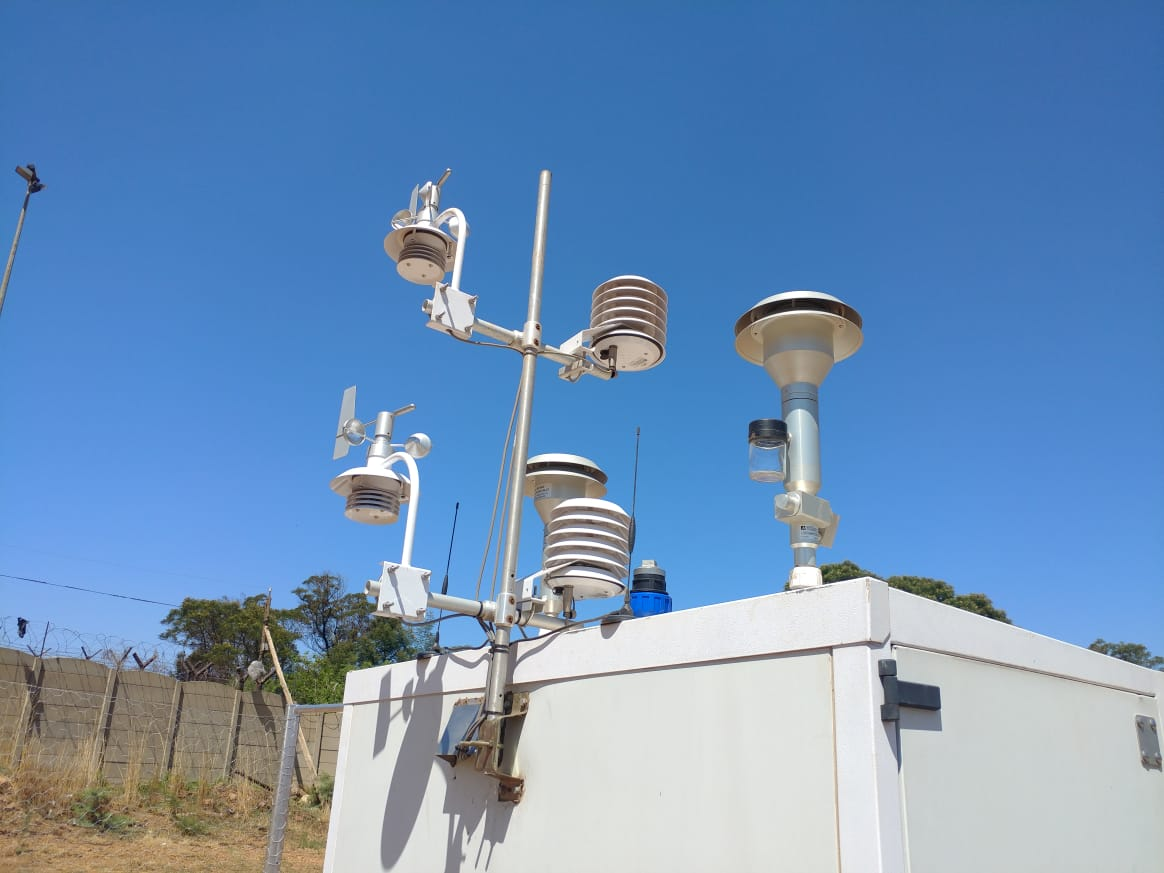
\includegraphics[width=\textwidth]{images/wedela.jpeg}
    \caption[Meteorological equipment deployed at Wedela.]{The MetOne MSO 232 instruments deployed at Wedela.}
    \label{fig:wadela_instruments_met}
\end{figure}

\begin{figure}[!htb]
    \centering
    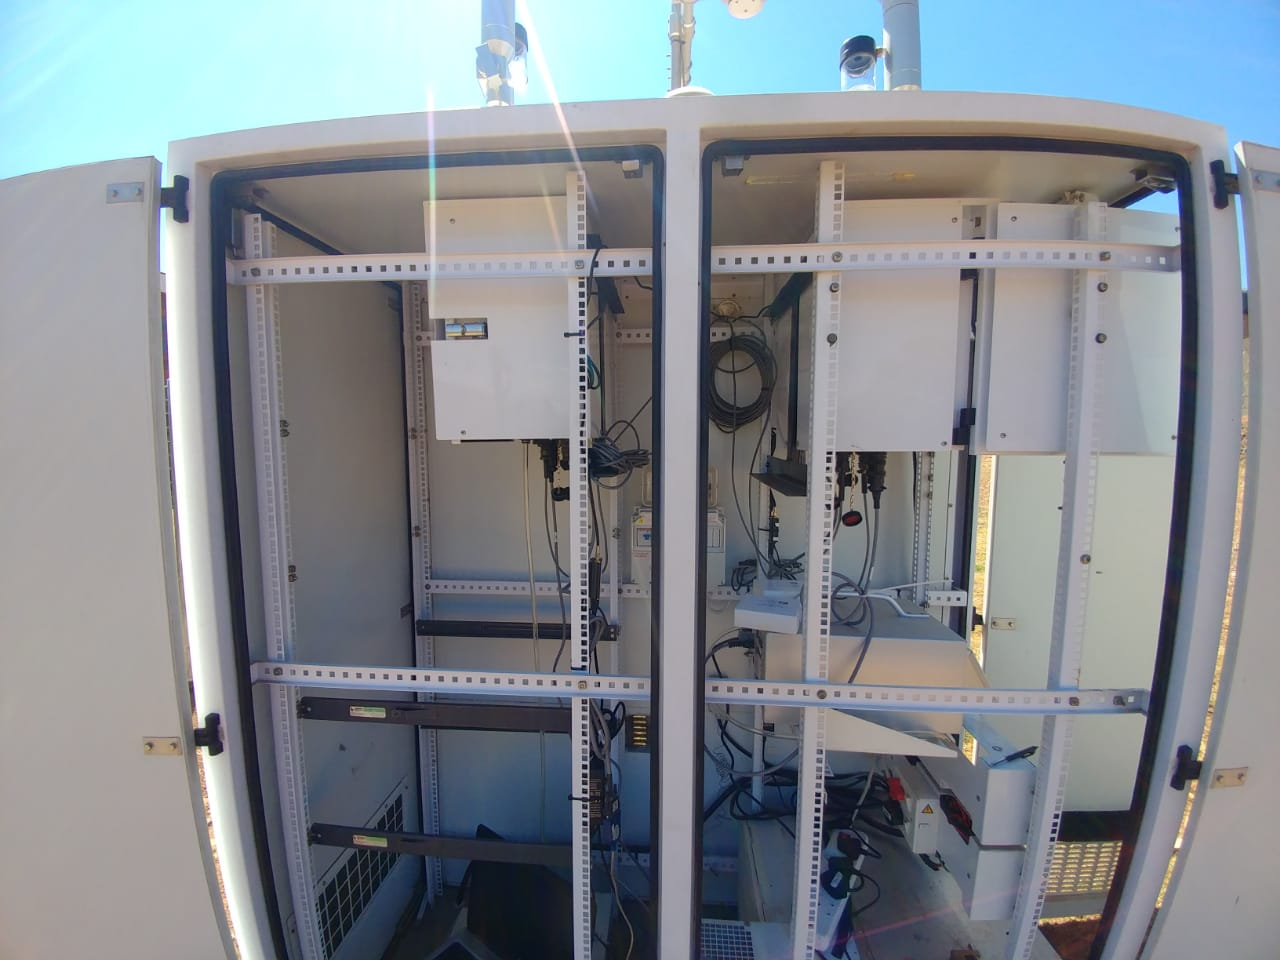
\includegraphics[width=\textwidth]{images/wadela_10.jpeg}
    \caption[Side view of $PM_{2.5}$ and $PM_{10}$ equipment deployed in Wedela.]{Side view of \gls{pm2.5} and \gls{pm10} equipment deployed in Wedela.}
    \label{fig:wadela_instruments_pm}
\end{figure}

\begin{figure}[!htb]
    \centering
    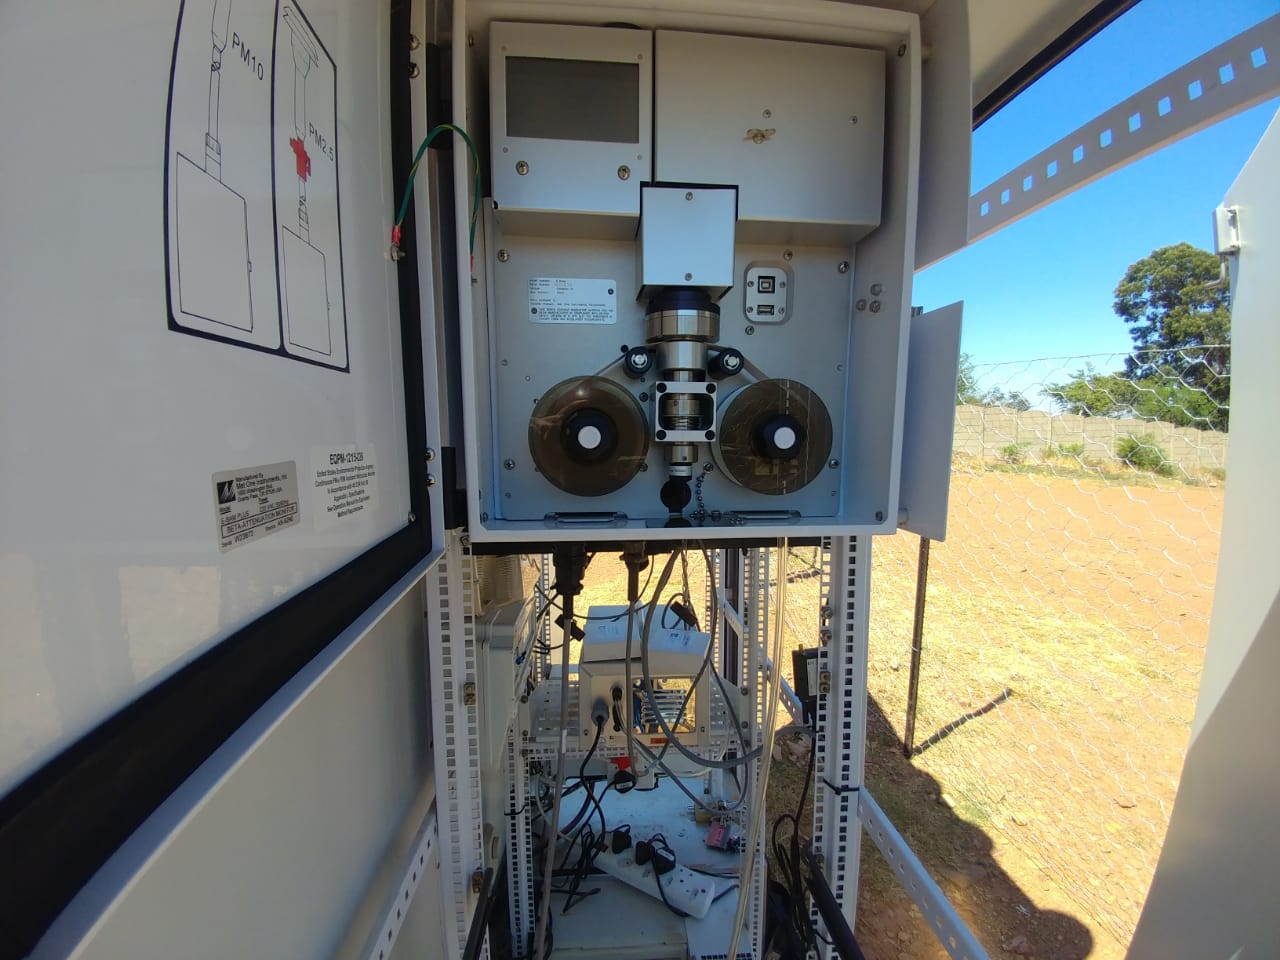
\includegraphics[width=\textwidth]{images/wedela_6.jpeg}
    \caption[Front view of $PM_{2.5}$ equipment deployed in Wedela.]{Front view of the \gls{pm2.5} equipment deployed in Wedela.}
    \label{fig:wadela_instruments_pm2}
\end{figure}
\section{Characterizing the chemical composition of ambient particulate matter in Wadela}

Samples will be collected for a two week period during winter and summer. Two samples a day will split the
typical bimodal ambient concentration peaks observed in low income communities in other regions. Sampling
will be undertaken using a \gls{sfu} sampler. The sampler collects particles which have an
\gls{aed} of less than \SI{10}{\micro\meter} in separate coarse and fine fractions. The
coarse fraction corresponds to aerosols collected with an \gls{aed} between \num{10} and \SI{2.5}{\micro\meter} while the fine fraction
corresponds to aerosols collected with an \gls{aed} lower than \SI{2.5}{\micro\meter}. Two 47-mm Nucelopore polycarbonate
filters with diameters of \SI{8.0}{\micro\meter} and \SI{0.4}{\micro\meter} were sequentially used during sampling.
After sampling, the nucleopore filters are stabilised 24 hours prior to weighing and then placed in a stabilised
environment prior to \gls{xrf} and \gls{ic} Analysis.

The extracts are analysed with a Metrohm 850 Professional IC. The Chromatograph has a Metrosep A Supp 15 Anion Membrane and a Metrosep C 4 250 Cation Membrane. The \gls{ic} analysis will be performed for the following anions and cations, F- , Cl- , Br- , NO3- , SO42- , PO43- , Na+ , NH4+ , K+ , Ca+ , Mg+ . All these procedures are conducted in a stabilized room to prevent any contamination. The results of particle composition analyses are necessary for identifying all the polluting sources that contributed to the collected samples \citep{Begum2017}. Source profiles obtained along with the chemical data for receptor samples are then constructed from literature.

\section{Apportion the contributing sources to the sampled ambient particulate loading in Wadela}

The chemical species present in atmospheric particulates reveals their sources. Geological material contains large abundances of Al, Si, K, Ca and Fe. While abundances of Al, K, Ca and Fe are similar among the source profiles in unpaved and paved road dust. Elemental carbon abundances are highly variable in geological material and are often negligible in natural soil samples while organic carbon is \SIrange{5}{15}{\percent} in geological profiles, being most abundant in paved road dust and agricultural dust. Motor vehicle emissions are likely contributors to Pb, EC and OC abundances observed in paved road dust. In general, abundances of SO42- , NO3- and NH4+ are low, falling in the range of \SIrange{0}{0.3}{\percent}. Na and Cl are also low, with less than \SI{0.5}{\percent} in abundance. Elemental and organic carbon are the most abundant species in motor vehicle exhaust, contributing to over 95\% of the total mass. However, Pb and Br abundances are low and highly variable. Zn was found in most vehicle exhaust profiles, although present at low abundance (0.05\% or less) (Watson et
al., 2004). Fine fraction particulate profiles undertaken by \cite{Watson1996} for residential wood
combustion, residential coal combustion and forest fires found average organic carbon abundances to range
from approximately 50\% in residential wood combustion and forest fire profiles to approximately 70\% in the
residential coal combustion profiles. Elemental carbon profiles averaged 3\%, 12\% and 26\% in forest fires,
residential wood combustion and residential coal combustion profiles, respectively. The organic carbon/total
carbon ratio was highest in the forest fire profile with a ratio of 0.94. Similar ratios were observed for
residential wood and coal combustion profiles, with 0.81 and 0.73 recorded, respectively (Watson et al.,
2004). Calloway et al (1989) found K+ /K ratios of 0.80 to 0.90 in burning profiles compared to the low ratios
measured in geological material. SO42- , NO3- and Si abundances in residential coal combustion are \num{2} to \num{4}
times higher than those in residential wood combustion and forest fire profiles.
Profiles for coal fired power generation differ substantially from residential coal combustion, despite the fuels
being similar, due to the different emission control technologies used. SO42- has very high abundances in the
particle phase while SO2 can be hundreds to thousands times higher than the particle mass. Crustal
elements such as Si, Ca and Fe in the coal-fired power generation profiles are present at \SIrange{30}{50}{\percent} of the
corresponding levels found in the geological material. Al is present at similar or higher levels in the power
generation profile as compared to the geological material. Other elements such as P, K, Ti, Cr, Mn, Sr, Zr and
Ba have less than \SI{1}{\percent} abundances. Se has also been detected at abundances of \SIrange{0.2}{0.4}{\percent} in coal fired
power station emissions which does not have scrubbers installed \citep{Watson1996}. Abundances of
SO42- , NO3- and NH4+ in directly emitted particles cannot account for the concentration of the species
measured in the atmosphere as ambient concentrations contain both primary and secondary particles. SO2 ,
NH4 and NOx are the precursors for sulfuric acid, ammonium bisulfate, ammonium sulfate, and ammonium
nitrate particles (Seinfeld, 1986; Watson et al., 1994). Several VOCs may also change into particles due to
photochemical transformation (Grosjean and Seinfeld, 1989). Several of these particles, notably those
containing ammonium nitrate, are volatile and transfer mass between the gas and particle phase to maintain
a chemical equilibrium (Stelson and Seinfeld, 1982a-c). This volatility has implications for ambient
concentration measurements as well as for gas and particle concentrations in the atmosphere.
Once the samples had been analysed, statistical receptor models were then applied to the aerosol data for
source apportionment purposes. Receptor modelling is used to characterise particulate air pollutant sources
and calculate each source contribution to a particular pollutant. There are two main techniques based on
chemical mass balance and multivariate statistics. \gls{cmb} uses both known profiles
of source emissions and ambient data from the measuring site while multivariate methods can only identify
sources from ambient measurements (Harrison and Yin, 2004). These models have been widely used for
aerosol source apportionment studies.

\gls{pca} is a statistical factor analysis method based on the law of conservation
of mass. It operates by first extracting a series of principal factors (components) from the measured data on
pollutant concentrations, on the basis of the mutual correlation between the different species. These are
then interpreted as putative sources, and the contribution from each estimated from the factor scores.
\gls{pca}is a multivariate modelling technique that does not need data on source compositions as inputs. It can
therefore be used to identify sources, and estimate contributions, where detailed information on source
characteristics is not available, but where a substantial amount of measured concentration data exists.
\gls{pca} is based on the analysis of the correlation between measured concentrations of chemical species in a
number of samples, assuming that highly correlated compounds come from the same source. The method
can thus be used to detect the hidden source information from ambient measurement datasets. Ambiguitiesinevitably arise during interpretation of the factors, and the validity of the interpretation depends on good
prior understanding of possible source characteristics; in the absence of such knowledge the results
obtained can thus be somewhat hypothetical and tentative.

\gls{pca} assumes that the composition of the emission sources is constant over the sampling period at the
receptors; chemical species do not interact with each other and their concentrations are linearly additive;
source profiles are linearly independent of each other; measurement errors are random and uncorrelated;
the number of species is greater than or equal to the number of sources; the number of samples is much
greater than the number of source types to ensure statistically meaningful calculations; variability of the
concentrations from sample to sample is primarily due to differences in source contribution and not due to
measurement uncertainty or changes in source composition; and the effect of processes that affect all
sources equally (e.g. atmospheric dispersion) is much smaller than the effect of processes that influence
individual sources (e.g. wind direction and changes in emission rates).

\gls{cmb} receptor models are used to apportion measured pollutant concentrations (or
exposures or doses) to their sources, and to assess the proportional contribution of each source. Chemical
mass balance models combine the chemical and physical characteristics of gases and particles measured at
the sources and receptors to both identify the presence of and to quantify source contributions to receptor
concentrations (Schauer et al., 2005). The \gls{cmb} receptor model was first applied by Winchester and Nifong
(1971), Hidy and Friedlander (1972), and Kneip et al (1973). The original applications used unique chemical
species associated with each source-type, the so-called “tracer” solution. Friedlander (1973) introduced the
ordinary weighted least-squares solution to the \gls{cmb} equations which had the advantages of relaxing the
constraint of a unique species in each source-type and of providing estimates of uncertainties associated
with the source contributions. Gordon (1980, 1988) and Kowalkzyk et al (1978) subsequently applied this
method to elemental concentrations measured in source and receptor samples. However, the ordinary
weighted least squares solution was limited in that only the uncertainties of the receptor concentrations were
considered while the uncertainties of the source profiles, which were usually much higher than the
uncertainties of the receptor concentrations, were not considered (Coulter, 2004). The ambient chemical
concentrations are expressed as the sum of the products of species abundances and source
contributions. The equations are solved for source contributions, using the ambient concentrations and
source profiles as inputs. \gls{cmb} models can be applied when the measured ambient concentration of different
species (Cij ) and the number of sources and their profiles (p and fpj) are known. The mass contribution
from each source to each sample (g ip ) is found by a least squares solution of the over determined system of
equations.

The \gls{cmb} model provides information on which combinations of profiles are likely to provide contributors by
means of statistical performance measures (Watson et al., 1991). The important measures that are
evaluated for each sample are: 1) the source contributions estimates and their uncertainties, 2) ‘chi-square’,
the weighted sum of the squares of the differences between calculated and measures species
concentrations (values between two and four indicate acceptable fits while values less than one indicate
good fits to the data), 3) ‘r-square’, the fraction of the variance in the measured concentrations accounted for
by the variance in the calculated species concentrations (values greater than 0.9 indicate a good fit to the
measured data) and 4) ‘percent mass’ or the percent of the total mass accounted for by the source
contribution estimates (values of between 80 – 120\% are considered to be good) (Kuhns et al., 2002).
The \gls{cmb} output also contains the ratios of calculated to measured concentration (C/M) and the ratio of the
difference between calculated and measured concentration divided by the uncertainty of this difference (R/U)
for each chemical species. These ratios are indicative of the fits of the individual species (Kuhns et al.,
2002). The ‘Eligible Space Dimension and Maximum Uncertainty’ clusters identify collinearity of similarity
between source profiles. This treatment (Henry, 1992) uses two parameters, maximum source uncertainty
and minimum source projection on the eligible space. The maximum source uncertainty determines the
eligible space to be spanned by the eigenvectors whose inverse singular values are less than or equal to the
maximum source uncertainty. The ‘Number of Estimable Sources’ are the source contributions that are
estimable given their source contributions and propagated uncertainties. Collinearity may result from small
source contribution estimates with relatively large uncertainties. The appearance of profiles in the eligible
space clusters does not invalidate the source contribution estimates. These clusters offer guidance that the
relative uncertainties of the source contribution estimates might be reduced by eliminating one or more of the
profiles or by linearly combining the profiles into a new profile that represents the combined contribution from
both source types (Kuhns et al., 2002).

The \gls{cmb} model assumes that all sources contributing significantly to measured concentrations are identified
and their emission source profiles are characterized; source profiles are constant over the receptor andsource sampling period; species included are not reactive (i.e. they add linearly); the number of sources or
source categories is less than the number of chemical species; source profiles are linearly independent of
each other and measurement uncertainties are random, uncorrelated and normally distributed (Coulter,
2004).

However, these assumptions are a limitation of the model as source compositions are not constant;
components do react with each other and systems are not linear; it is generally not known how many
sources are contributing to a receptor; there are more sources than components which can be practically
measured; many sources have very similar compositions; measurement errors are not necessarily random,
uncorrelated or normally distributed and few sources have their own unique tracer components (Watson,
1984).

\section{Realtime data access}

A real-time monitoring solution has been established through \url{www.ecostat.co.za} to
the EBAM \gls{pm2.5} and \gls{pm10} instruments located in Wadela. Ecostat allows users to access the data
through any browser such as Firefox, Chrome or Internet Explorer. 

\begin{itemize}
\item Login name: Anglo
\item Login password: NWU1
\end{itemize}

Ecostat has various functions to enable data monitoring in real-time, this includes
viewing the status of the data logging as seen in \hyperref[fig:ecostat_status]{figure \ref{fig:ecostat_status}}. The status reports assists the project technical staff to avoid
unnecessary travel while researchers can access the raw data to do quality control checks. 

\begin{figure}[!htb]
    \centering
    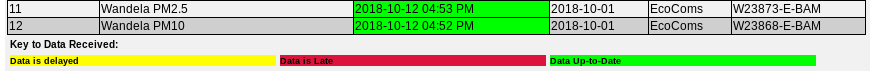
\includegraphics[width=\textwidth]{images/ecstat_status.png}
    \caption[A screenshot of the ecostat status report.]
    {A screenshot of the ecostat status report.}
    \label{fig:ecostat_status}
\end{figure}

Ecostat further allows quick view products of the instrument status,
meteorological and pollution data from the site location as seen
in \hyperref[fig:ecostat_quick]{figure \ref{fig:ecostat_quick}}. This is
valuable to quickly asses current ambient environment and also to check the
instrument for unrealistic or erroneous values.

\begin{figure}[!htb]
    \centering
    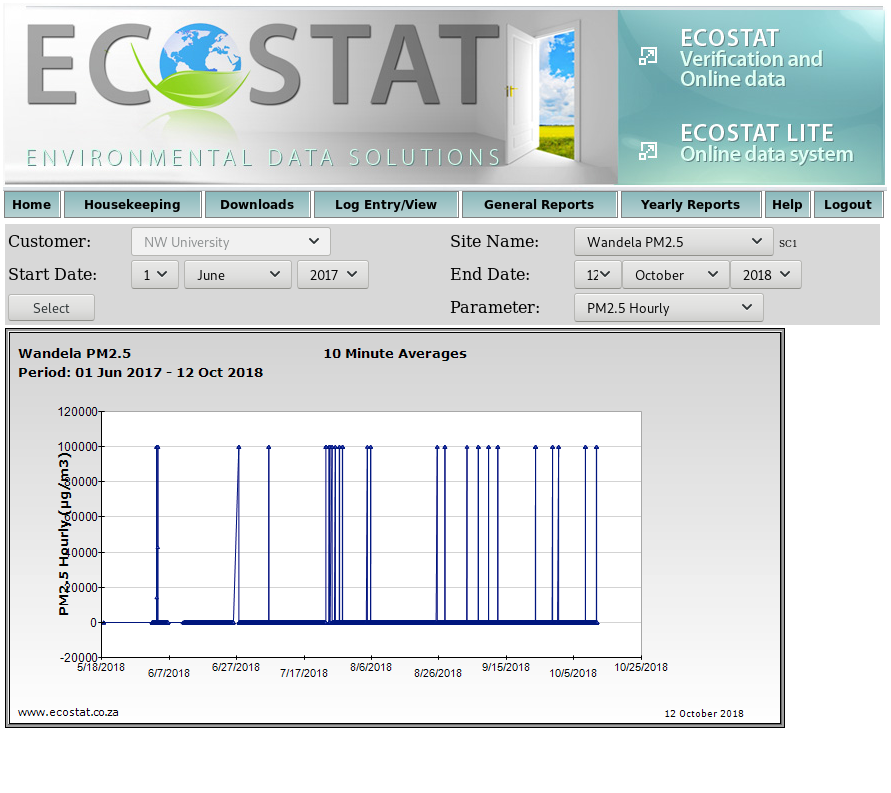
\includegraphics[width=\textwidth]{images/ecostat_quick.png}
    \caption[Online interface to the realtime data.]{The ecostat interface used to provide realtime access to the monitoring data.}
    \label{fig:ecostat_quick}
\end{figure}

\section{File conventions}

All final datasets are stored in \gls{ascii} format with extensions
``.txt'' and ``.csv''. This is the most
widely accepted format readable by most software. The most common
convention is simple \gls{csv}, usually denoted with the extension
``.csv''. Most of the data acquisition devices
store data in \gls{ascii}, these raw files are kept untouched. All
binary formats are converted into \gls{csv} files. Staring all
data-sets in \gls{ascii} will ensure that all users will have easy
access to the data and any future changes to commercial software will
not impact on its accessibility.

Excel is the most common software used for data processing. \gls{csv}
files easily integrates with most import and export facilities of
Excel. Special care must be taken when using the following features:

\begin{description}
\item [Importing files] A field separator should be chosen when
  importing files into Excel. The default separator is a comma
  (,). This implies that a comma should not be used anywhere in data
  files other than for denoting a field separator. It is very likely
  that commas will be present if there are long strings or written
  descriptions in a file. In these cases, a pipe (\textbar) can be used as a
  separator. These instances should be avoided as far as possible.
\item [Formatting of cells] Care must be exercised when processing or
  formatting data in excel. The formatting of each cell in Excel
  depends on the settings. It frequently looks different from the raw
  data. If the user are not aware of the current formatting setting of
  the cell, row or column, mistakes will be made when importing or
  exporting data. The most common places for these mistakes comes when
  dealing with dates, times, percentages and decimal characters.
\item [Exporting files] Final data-sets is stored in \gls{csv}. This is
  a standard export feature of Excel. The following features of most
  current versions of Excel must be taken into consideration when
  exporting files to \gls{csv}. If the Excel files contains many
  sheets, only the active sheet will be saved to \gls{csv} per export
  action. Each sheet must therefore be saved to a separate file.
\item [Using inverted commas (``)] Inverted commas typically has a
  special meaning in Excel. It is used to denote a text string for
  that particular field. When encapsulating data points in inverted
  commas, the user invariable forces Excel to see that field as a text
  string. This will be problematic if the user wishes to use that
  field in any operations, like algebraic conversion or time series
  operations. For this reason, inverted commas should only be used to
  denote text strings. An example would be to prevent excel from splitting a
  long text description containing commas into fields when importing a
  \gls{csv} files with a comma as a separator.
\end{description}

\subsubsection{General procedure for data quality control}
The raw data-sets collected are merged and processed into a final data
set for analysis through the following steps:

\begin{enumerate}
\item Apply date and time corrections to each of the raw data files
  using the instrument logs
\item Merge each of the data-sets above into one uniform data-set
\item Apply masks to each instrument according to the instrument log
\item Perform automated quality control on each variable and flag problematic values
  \begin{itemize}
   \item Test for sensible observation date and time values.
   \item Flag data close to or below the instrument detection limit. 
   \item Flag data close to or above the instrument's maximum detectable limited
   \item Test the gradient of each instrument against realistic response times
   \item Test for spikes by comparing with values before and after
   \item Test for stuck values and set missing
   \item Flag climatological outliers
   \item Flag outliers using the median absolute deviation
  \end{itemize}
\item Each variable with its associated flags identified in the automated quality control is then reviewed manually by viewing time series plots. Each flag is carefully inspected and values are deemed real or set to missing if a problem is suspected.
\item Values close to or below the detection limit are finally set to the minimum detection limit of the particular instrument \citep{Croghan2003}.
\end{enumerate}

The general philosophy in quality assuring data is to aggressively
ignore data that are suspected to be from a faulty instrument. Extra
care is taken when dealing with extreme values and outliers. These are
not set to missing unless they are part of a time period where the
instrument did not appear to be operating optimally.

\subsubsection{General procedure for data quality control}
The raw data-sets collected are merged and processed into a final data
set for analysis through the following steps:

\begin{enumerate}
\item Apply date and time corrections to each of the raw data files
  using the instrument logs
\item Merge each of the data-sets above into one uniform data-set
\item Apply masks to each instrument according to the instrument log
\item Perform automated quality control on each variable and flag problematic values
  \begin{itemize}
   \item Test for sensible observation date and time values.
   \item Flag data close to or below the instrument detection limit. 
   \item Flag data close to or above the instrument's maximum detectable limited
   \item Test the gradient of each instrument against realistic response times
   \item Test for spikes by comparing with values before and after
   \item Test for stuck values and set missing
   \item Flag climatological outliers
   \item Flag outliers using the median absolute deviation
  \end{itemize}
\item Each variable with its associated flags identified in the automated quality control is then reviewed manualy by viewing time series plots. Each flag is carefully inspected and values are deemed real or set to missing if a problem is suspected.
\item Values close to or below the detection limit are finally set to the minimum detection limit of the particular instrument \citep{Croghan2003}.
\end{enumerate}

The general philosophy in quality assuring data is to aggressively
ignore data that are suspected to be from a faulty instrument. Extra
care is taken when dealing with extreme values and outliers. These are
not set to missing unless they are part of a time period where the
instrument did not appear to be operating optimally.
%%%%%%%%%%%%%%%%%%%%%%%%%%%%%%%%%%%%%%%%%%%%%%%%%%%%%%%%%%%%%

\chapter{Site preparation and installation}
\label{sec:site}

Wedela is a small, low income settlement located in the Gauteng province of
South-Africa (26$^\circ$27'58"S 27$^\circ$23'0"E). The settlement is in close proximity to Carltonville
and also less than 80km from Johannesburg, the area is also known for the various goldmines
that operate in the area. \hyperref[fig:wadela]{Figure \ref{fig:wadela}}
indicates the relative position of Wedela in South-Africa and in proximity to other major
in the region.

\begin{figure}[!htb]
    \centering
    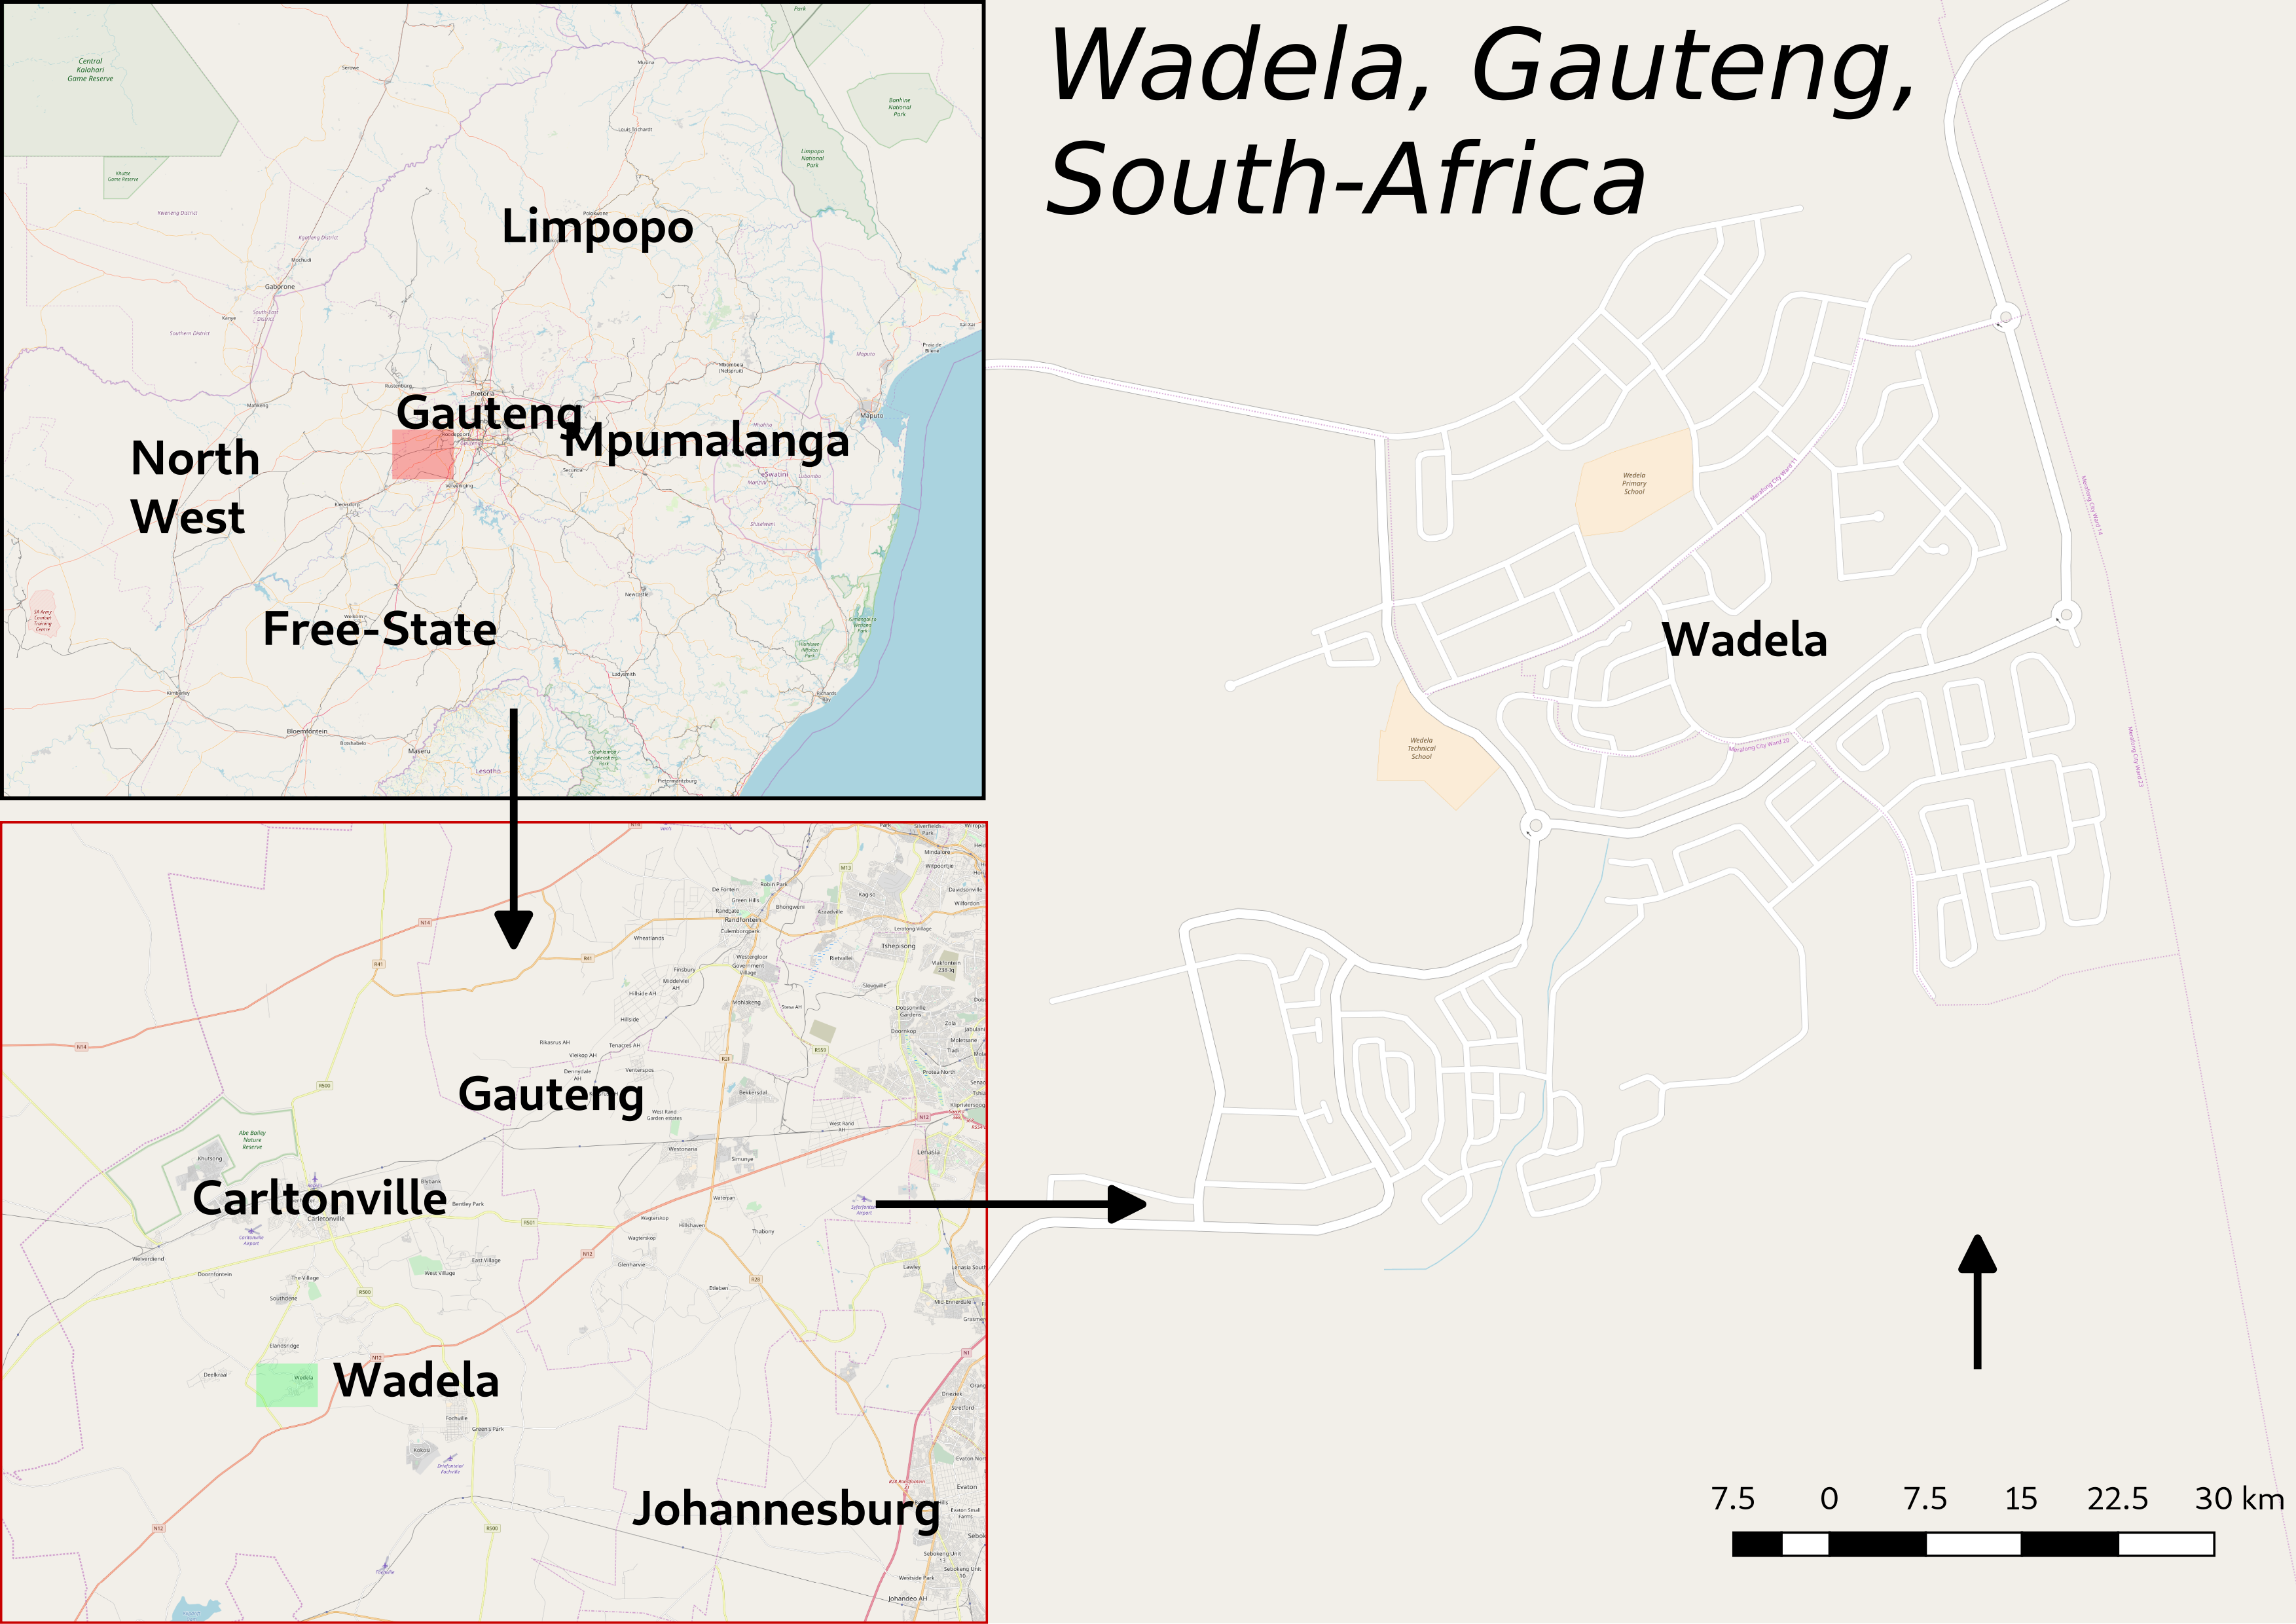
\includegraphics[width=\textwidth]{images/study_area_qgis.png}
    \caption[Study area: Wedela, Gauteng]{Wedela, seen in the above map, is the location where
    the study was conducted. The settlement is located in close proximity to Carltonville and Johannesburg.
    There is also various gold mines present in the region. The map shows Wedela's relative position in
    South-Africa as indicated in the overlay maps.}
    \label{fig:wadela}
\end{figure}

A site was identified at the Wedela Primary school that was located in the center of the settlement. The site also presented good security and a potential source of electricity. Access was negotiated through the pricipal of the school. Cables were installed for electricity and a fence errected for security (Figure~\ref{fig:wadela_fence}). Only technicians and research staff have access to the site.

\begin{figure}[!htb]
    \centering
    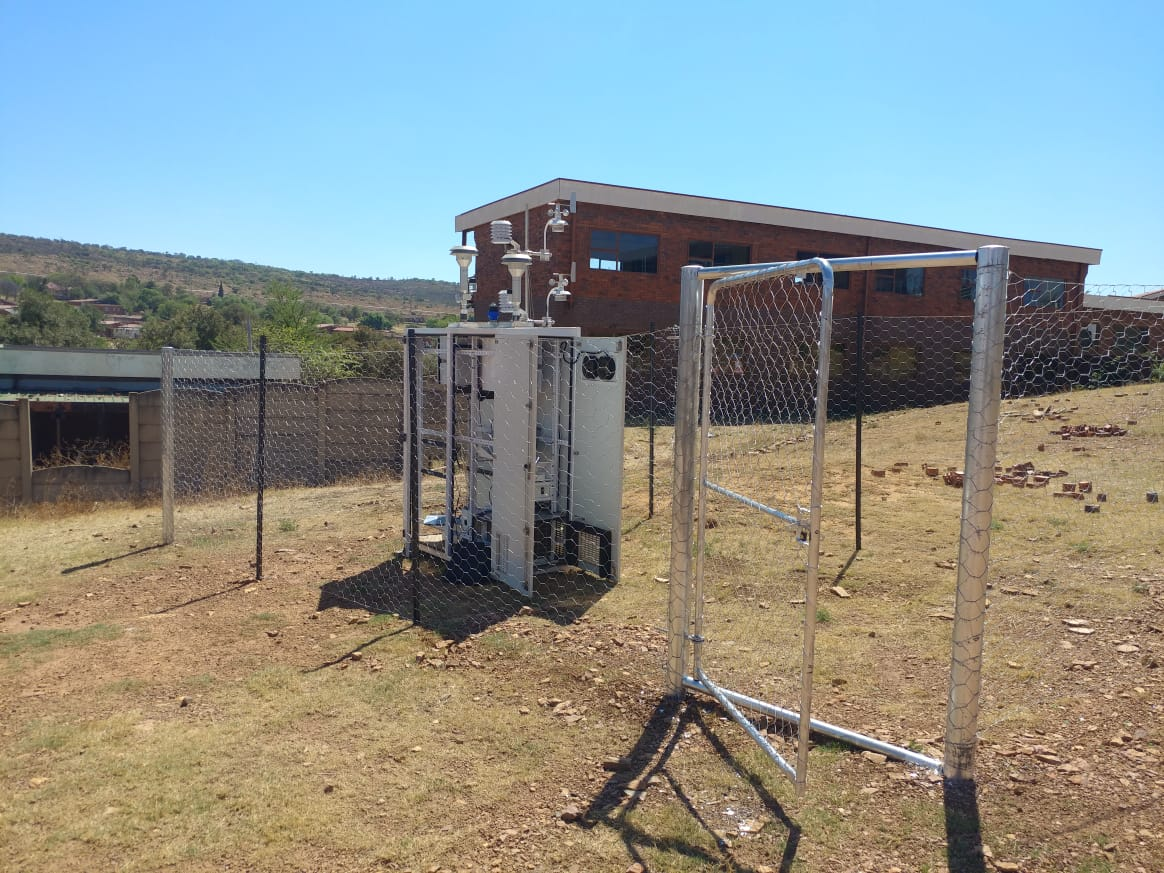
\includegraphics[width=\textwidth]{images/wedela_4.jpeg}
    \caption[Security and access control at the Wedela measuring site]{Security and access control at the Wedela measuring site}
    \label{fig:wadela_fence}
\end{figure}

The best meteorological data that can provide a characterization of the Wedela climate can be found at the Potchefstroom \gls{saws} weather station. This station has data since 1903. A climatology is presented in Table~\ref{table:potch_climate}.

\begin{table}
\scriptsize
\caption[Rainfall climate statistics for the SAWS station at Potchefstroom]{Rainfall climate statistics for the SAWS station at Potchefstroom (AGR), located at -26.733333,27.083333 for the period 1903-1984.}
\label{table:potch_climate}
\begin{center}
\begin{tabular}{ c c c c c c c c c c c c c c c c }
\toprule
%-------------------------------------------------------------------------------------------
\multirow{5}{*}[-1.5em]{\rotatebox[origin=c]{90}{\bfseries Month} } & 
\multicolumn{7}{c}{\multirow{2}{*}{\bfseries Precipitation (mm)}} &
\multicolumn{8}{c}{\bfseries Frequencies} \\
%-------------------------------------------------------------------------------------------
& & & & & & & & \multicolumn{8}{c}{\bfseries No of days with} \\
%-------------------------------------------------------------------------------------------
& \multirow{2}{*}{\rotatebox[origin=c]{90}{\bfseries Average }} & 
   & & 
  \multicolumn{2}{c}{\multirow{2}{*}{\begin{minipage}{1.75cm} \bfseries Highest Monthly \\ Max \& Date \end{minipage}}} &
  \multicolumn{2}{c}{\multirow{2}{*}{\begin{minipage}{1.75cm} \bfseries Lowest Monthly Max \& Date \end{minipage}}} &
  \multicolumn{7}{c}{\bfseries Precipitation} & \multirow{2}{*}{\rotatebox[origin=c]{90}{\bfseries Hail}} \\
%-------------------------------------------------------------------------------------------
 & & \multicolumn{2}{c}{\bfseries Max in 24h}  & & & & & 
\multicolumn{3}{c}{$\geq$\num{0.1}\si{\milli\meter}} & 
\multicolumn{3}{c}{$\geq$\num{1.0}\si{\milli\meter}} & 
$\geq$ \num{10}\si{\milli\meter} & \\
%-------------------------------------------------------------------------------------------
 & $\Sigma$ & \si{\milli\meter} & Date & $\Sigma_x$ & Date & $\Sigma_H$ & Date& 
 \rotatebox[origin=l]{90}{\bfseries Ave } & 
 \rotatebox[origin=l]{90}{\bfseries Max} & 
 \rotatebox[origin=l]{90}{\bfseries Min} & 
 \rotatebox[origin=l]{90}{\bfseries Ave} & 
 \rotatebox[origin=l]{90}{\bfseries Max} & 
 \rotatebox[origin=l]{90}{\bfseries Min} & 
 \rotatebox[origin=l]{90}{\bfseries Ave} & 
 \rotatebox[origin=l]{90}{\bfseries Ave} \\
%1 & 2 &3 &4 &5 &6 &7 &8 &9 &10 &11 &12 &13 &14 &15 &16 \\
\midrule 
P&80&51&&80&&80&&80&33&33&80&53&53&80&26\\
\midrule 
1&111&95&1977/31&258&1976&29&1933&13.2&19&6&9.9&17&4&3.6&0.4\\
2&95&79&1983/28&227&1907&8&1984&10.1&16&4&8.1&13&2&3.1&0.2\\
3&81&78&1975/18&276&1921&8&1983&10.2&17&4&8&15&3&2.7&0.3\\
4&46&83&1965/13&160&1971&0&1944&7.7&17&2&5&12&0&1.8&0.3\\
5&19&44&1950/03&99&1936&0&1982&3.8&10&1&2.5&8&0&0.7&0.2\\
6&8&61&1944/13&104&1944&0&1982&1.5&6&0&1&5&0&0.2&0.1\\
7&8&41&1957/02&83&1918&0&1981&1.5&9&0&1&8&0&0.2&0\\
8&9&39&1979/20&100&1922&0&1982&1.5&7&0&1&6&0&0.2&0\\
9&18&53&1940/25&93&1940&0&1983&3.5&12&0&2&11&0&0.6&0.3\\
10&50&72&1951/20&171&1913&1&1919&7.8&16&3&5.4&12&1&1.5&0.7\\
11&79&83&1939/03&170&1936&10&1941&12&21&3&8.3&18&1&2.7&0.5\\
12&101&140&1943/12&237&1909&21&1948&12.7&19&7&8.9&16&2&3.7&0.3\\
\midrule 
A&625&140&1943&980&1976&365&1903&85.5&&&61.1&&&21&3.3\\
\bottomrule
\end{tabular}
\end{center}
\end{table}

%%%%%%%%%%%%%%%%%%%%%%%%%%%%%%%%%%%%%%%%%%%%%%%%%%%%%%%%%%%%%

\chapter{Ambient monitoring}
\label{sec:ambient}

The initial results for the continuous ambient monitoring are presented in this chapter. The instruments were installed at the end of May 2018 and data are presented till the end of January 2019. Ambient \gls{pm} concentrations are compared against the national ambient standards as defined in \cite{RSA2009a} (see Table~\ref{table:naaqs}). The raw timeseries of the most important parameters are presented in Figure~\ref{fig:summary}. The data recovery and distribution of data are also presented.

Unreliable power supply continues to hamper data recovery in Wedela. The following major incidents caused futher data loss. The \gls{pm10} E-BAM was removed and taken for repair between 19 and 26 October 2018. The cable was damaged and all instruments lost data for a 2 week period in the end of November 2018. The \gls{pm10} E-BAM had tape advance problems in December 2018. The \gls{pm10} E-BAM sustained water damage on 10 January 2019 and was removed for repair. It has since been returned to the site.

\begin{table}[!htbp]
\caption[National ambient air quality standards]{National ambient air quality standards \citep{RSA2009a}}
\label{table:naaqs}
\begin{center}
\begin{tabular}{l r r} 
\toprule 
\bfseries Averaging &                          & \bfseries Frequncy of \\
\bfseries Period    &  \bfseries Concentration & \bfseries Exceedance  \\
\midrule 
\multicolumn{3}{l}{\bfseries Particulate Matter ($PM_{10}$)} \\
24 hours &  \SI{75}{\micro\gram\per\cubic\meter} & 4 \\
Annual   &  \SI{40}{\micro\gram\per\cubic\meter} & 0 \\
\multicolumn{3}{l}{\bfseries Particulate Matter ($PM_{2.5}$)} \\
24 hours & \SI{40}{\micro\gram\per\cubic\meter} & 4 \\
Annual   & \SI{20}{\micro\gram\per\cubic\meter} & 0 \\
\bottomrule 
\end{tabular}
\end{center}
\end{table}

\begin{figure}[!htb]
    \centering
    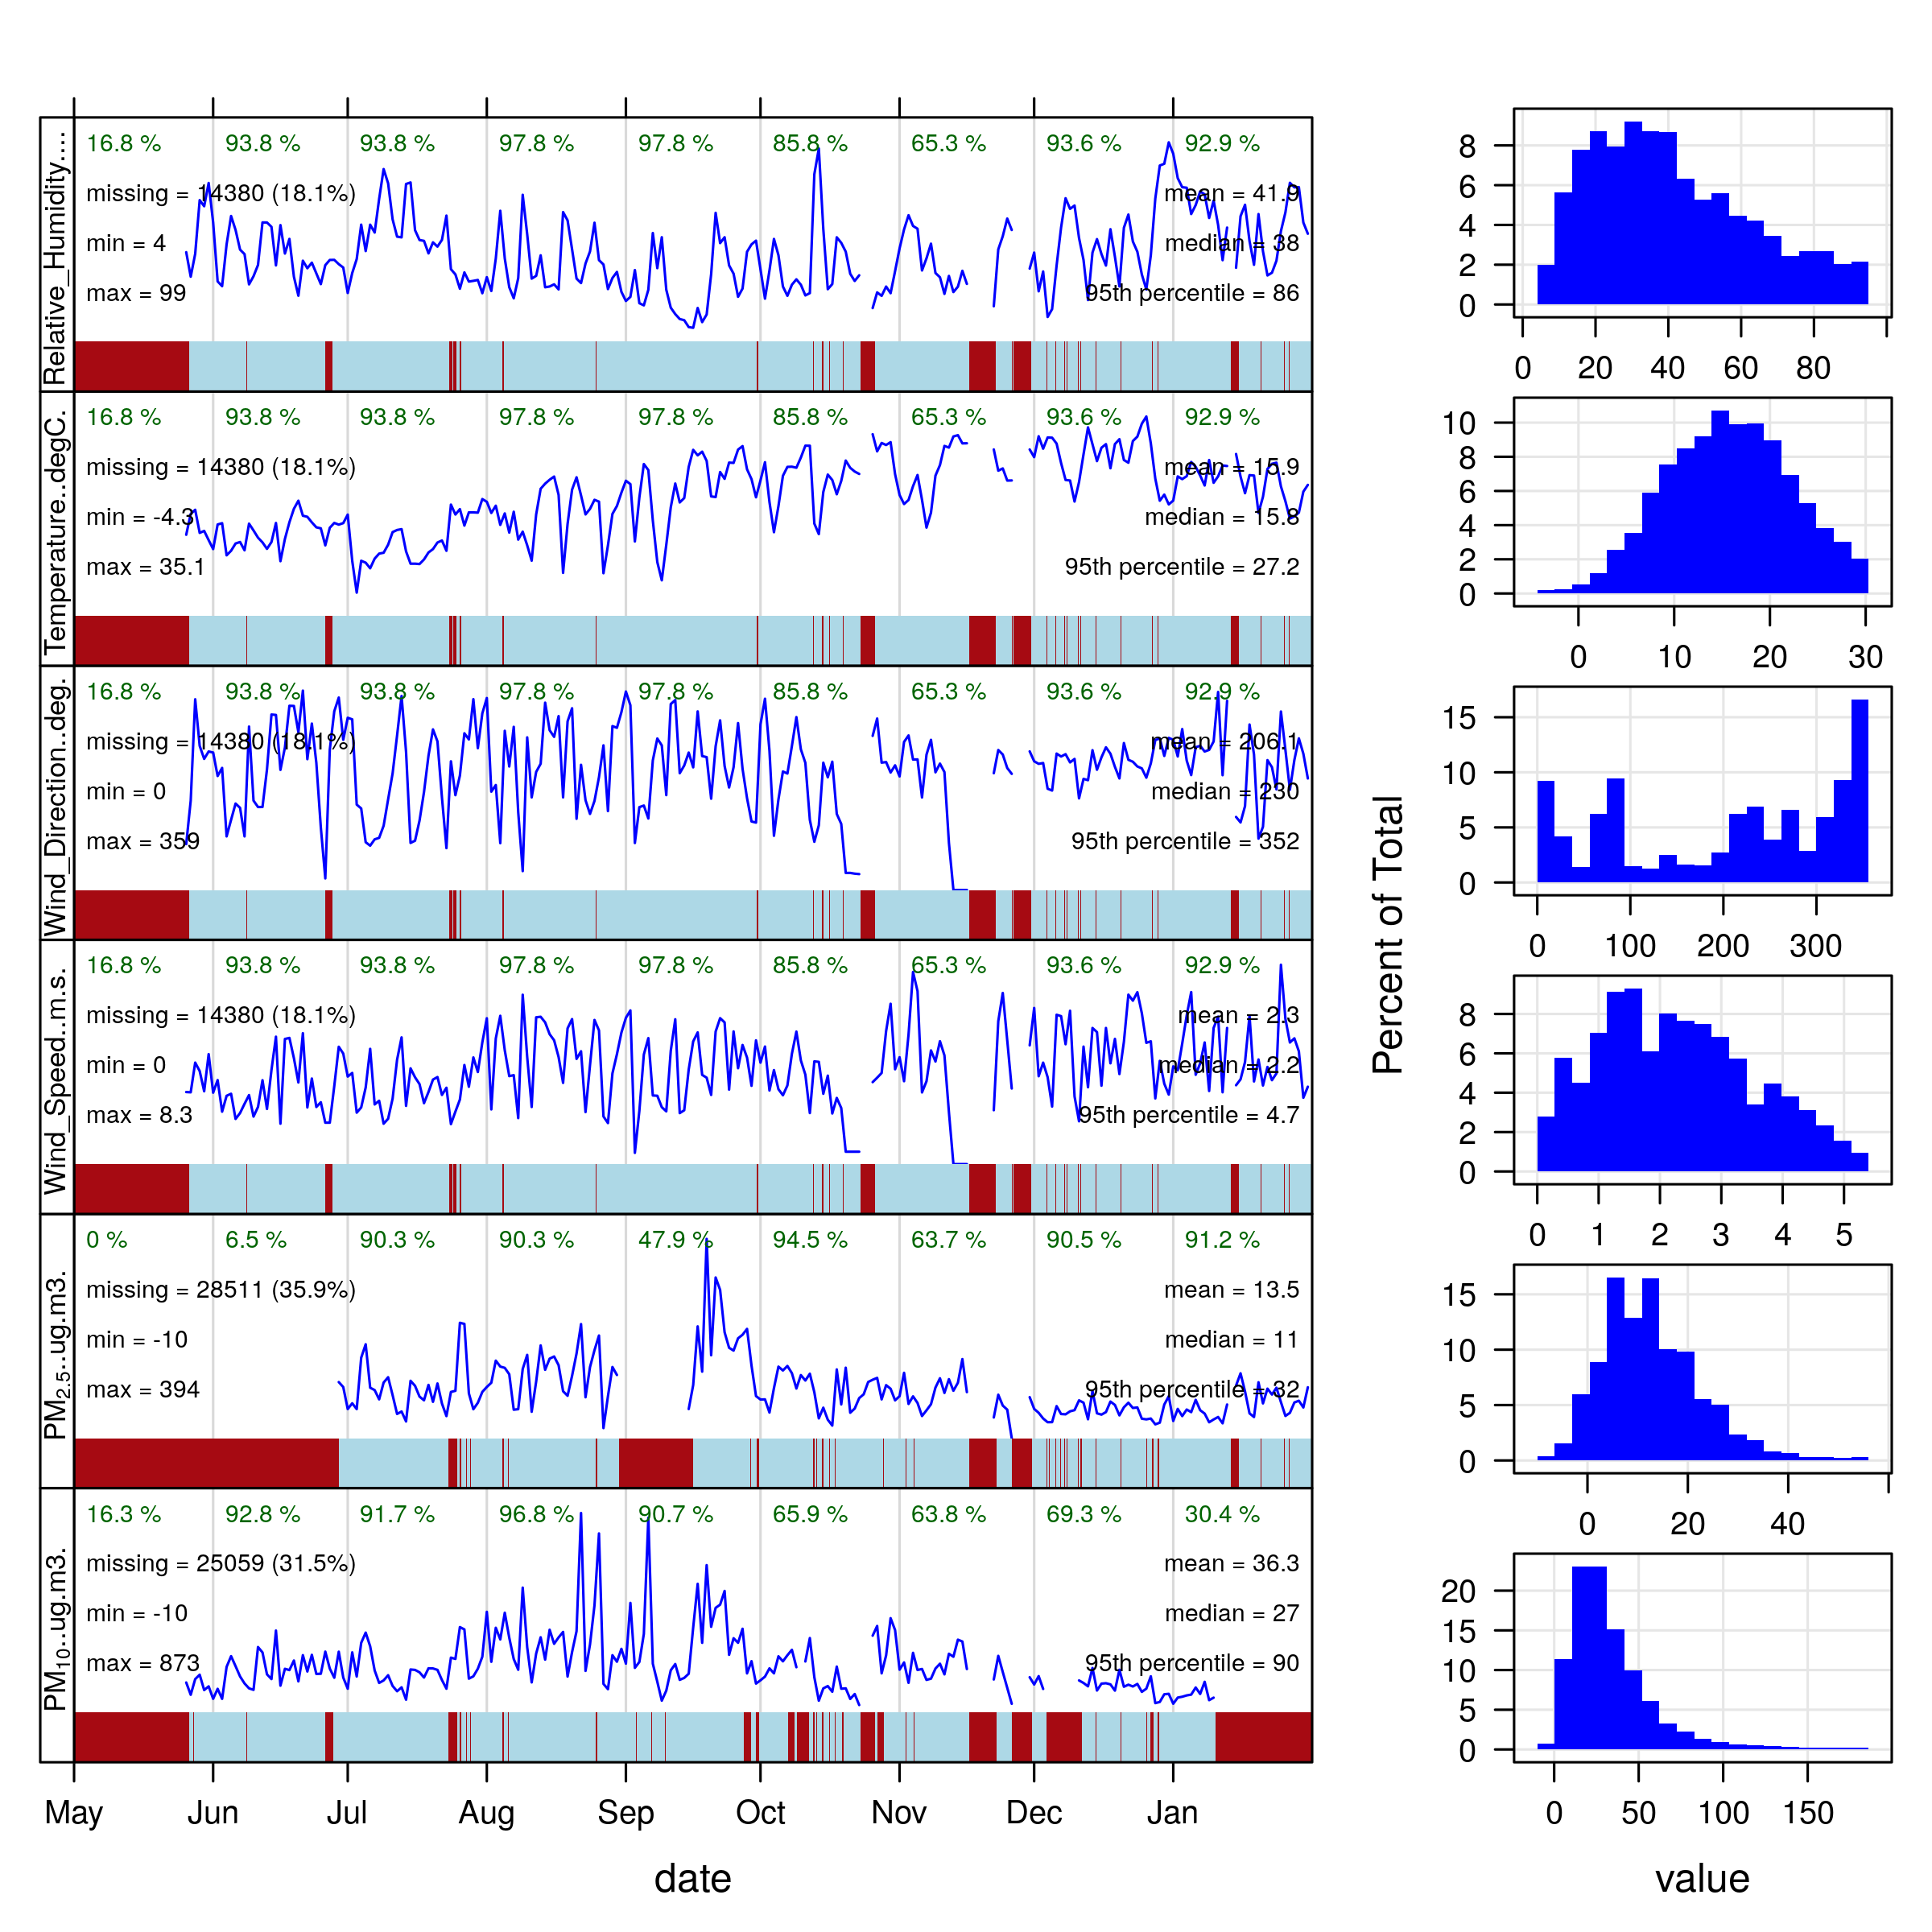
\includegraphics[width=\textwidth]{images/Wedela-ams.png}
    \caption[Time series of main parameters measured at Wedela.]{Time series and statistics of the main parameters monitored at Wedela between May 2018 and January 2019.}
    \label{fig:summary}
\end{figure}

\section{Meteorological measurements}

Meteorological data was captured at Wedela include temperature, relative humidity, pressure and winds. The variability of temperature (Figure~\ref{fig:summary-tmp}) and humidity (Figure~\ref{fig:summary-rh}) shows characteristic diurnal and seasonal variability. The dominant wind direction are northerly and northeasterly for most of the year, apart for November and December where a southwesterly component dominate (Figure~\ref{fig:windrose-monthly}). The diurnal distribution of with wind profile is similar with northeasterly directions dominating during the daylight hours and south westerlies also being prominent in the mornings (Figure~\ref{fig:windrose-hourly}). The diurnal and seasonal variation in wind speed is shown in Figure~\ref{fig:timevary-winds}. Wind speeds peak during the day with a minima shortly after sunset. August and September, and again November and December feature higher than normal wind speeds.

\begin{figure}[!htb]
    \centering
    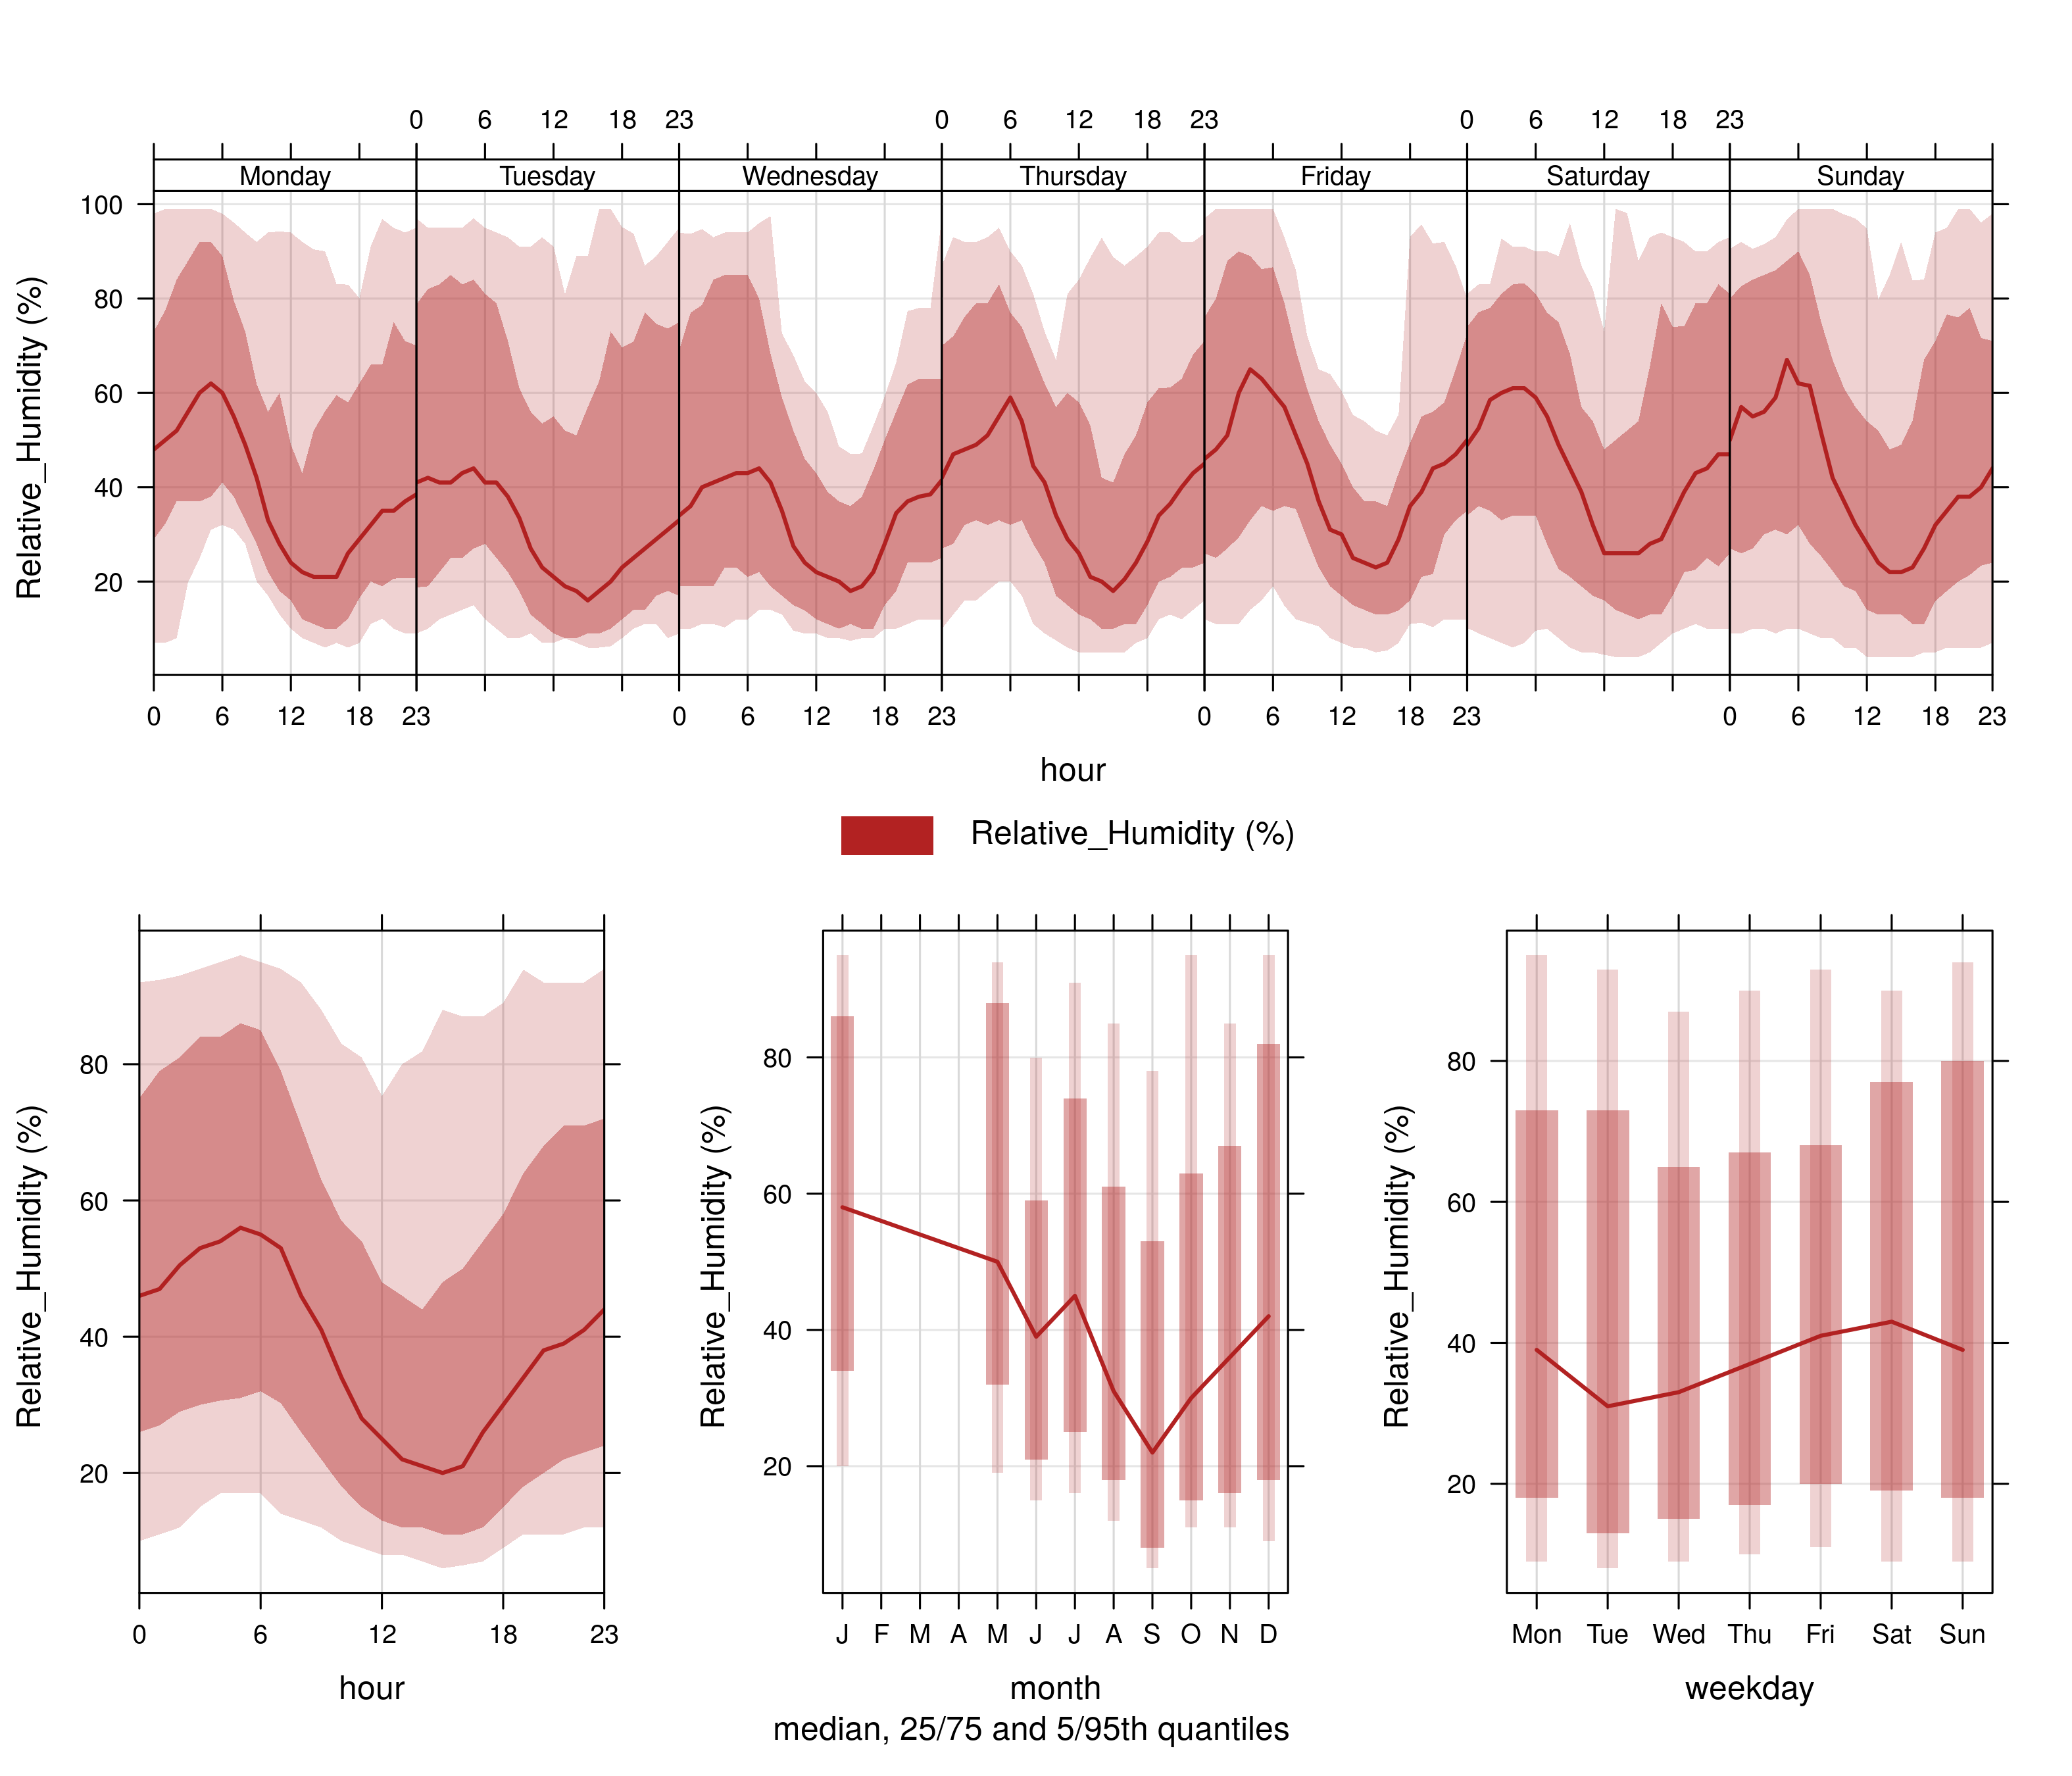
\includegraphics[width=\textwidth]{images/Wedela_Relative_Humidity_timevary.png}
    \caption[Time variation of relative humidity measurements at Wedela.]{Time variation of relative humidity measurements at Wedela.}
    \label{fig:summary-rh}
\end{figure}

\begin{figure}[!htb]
    \centering
    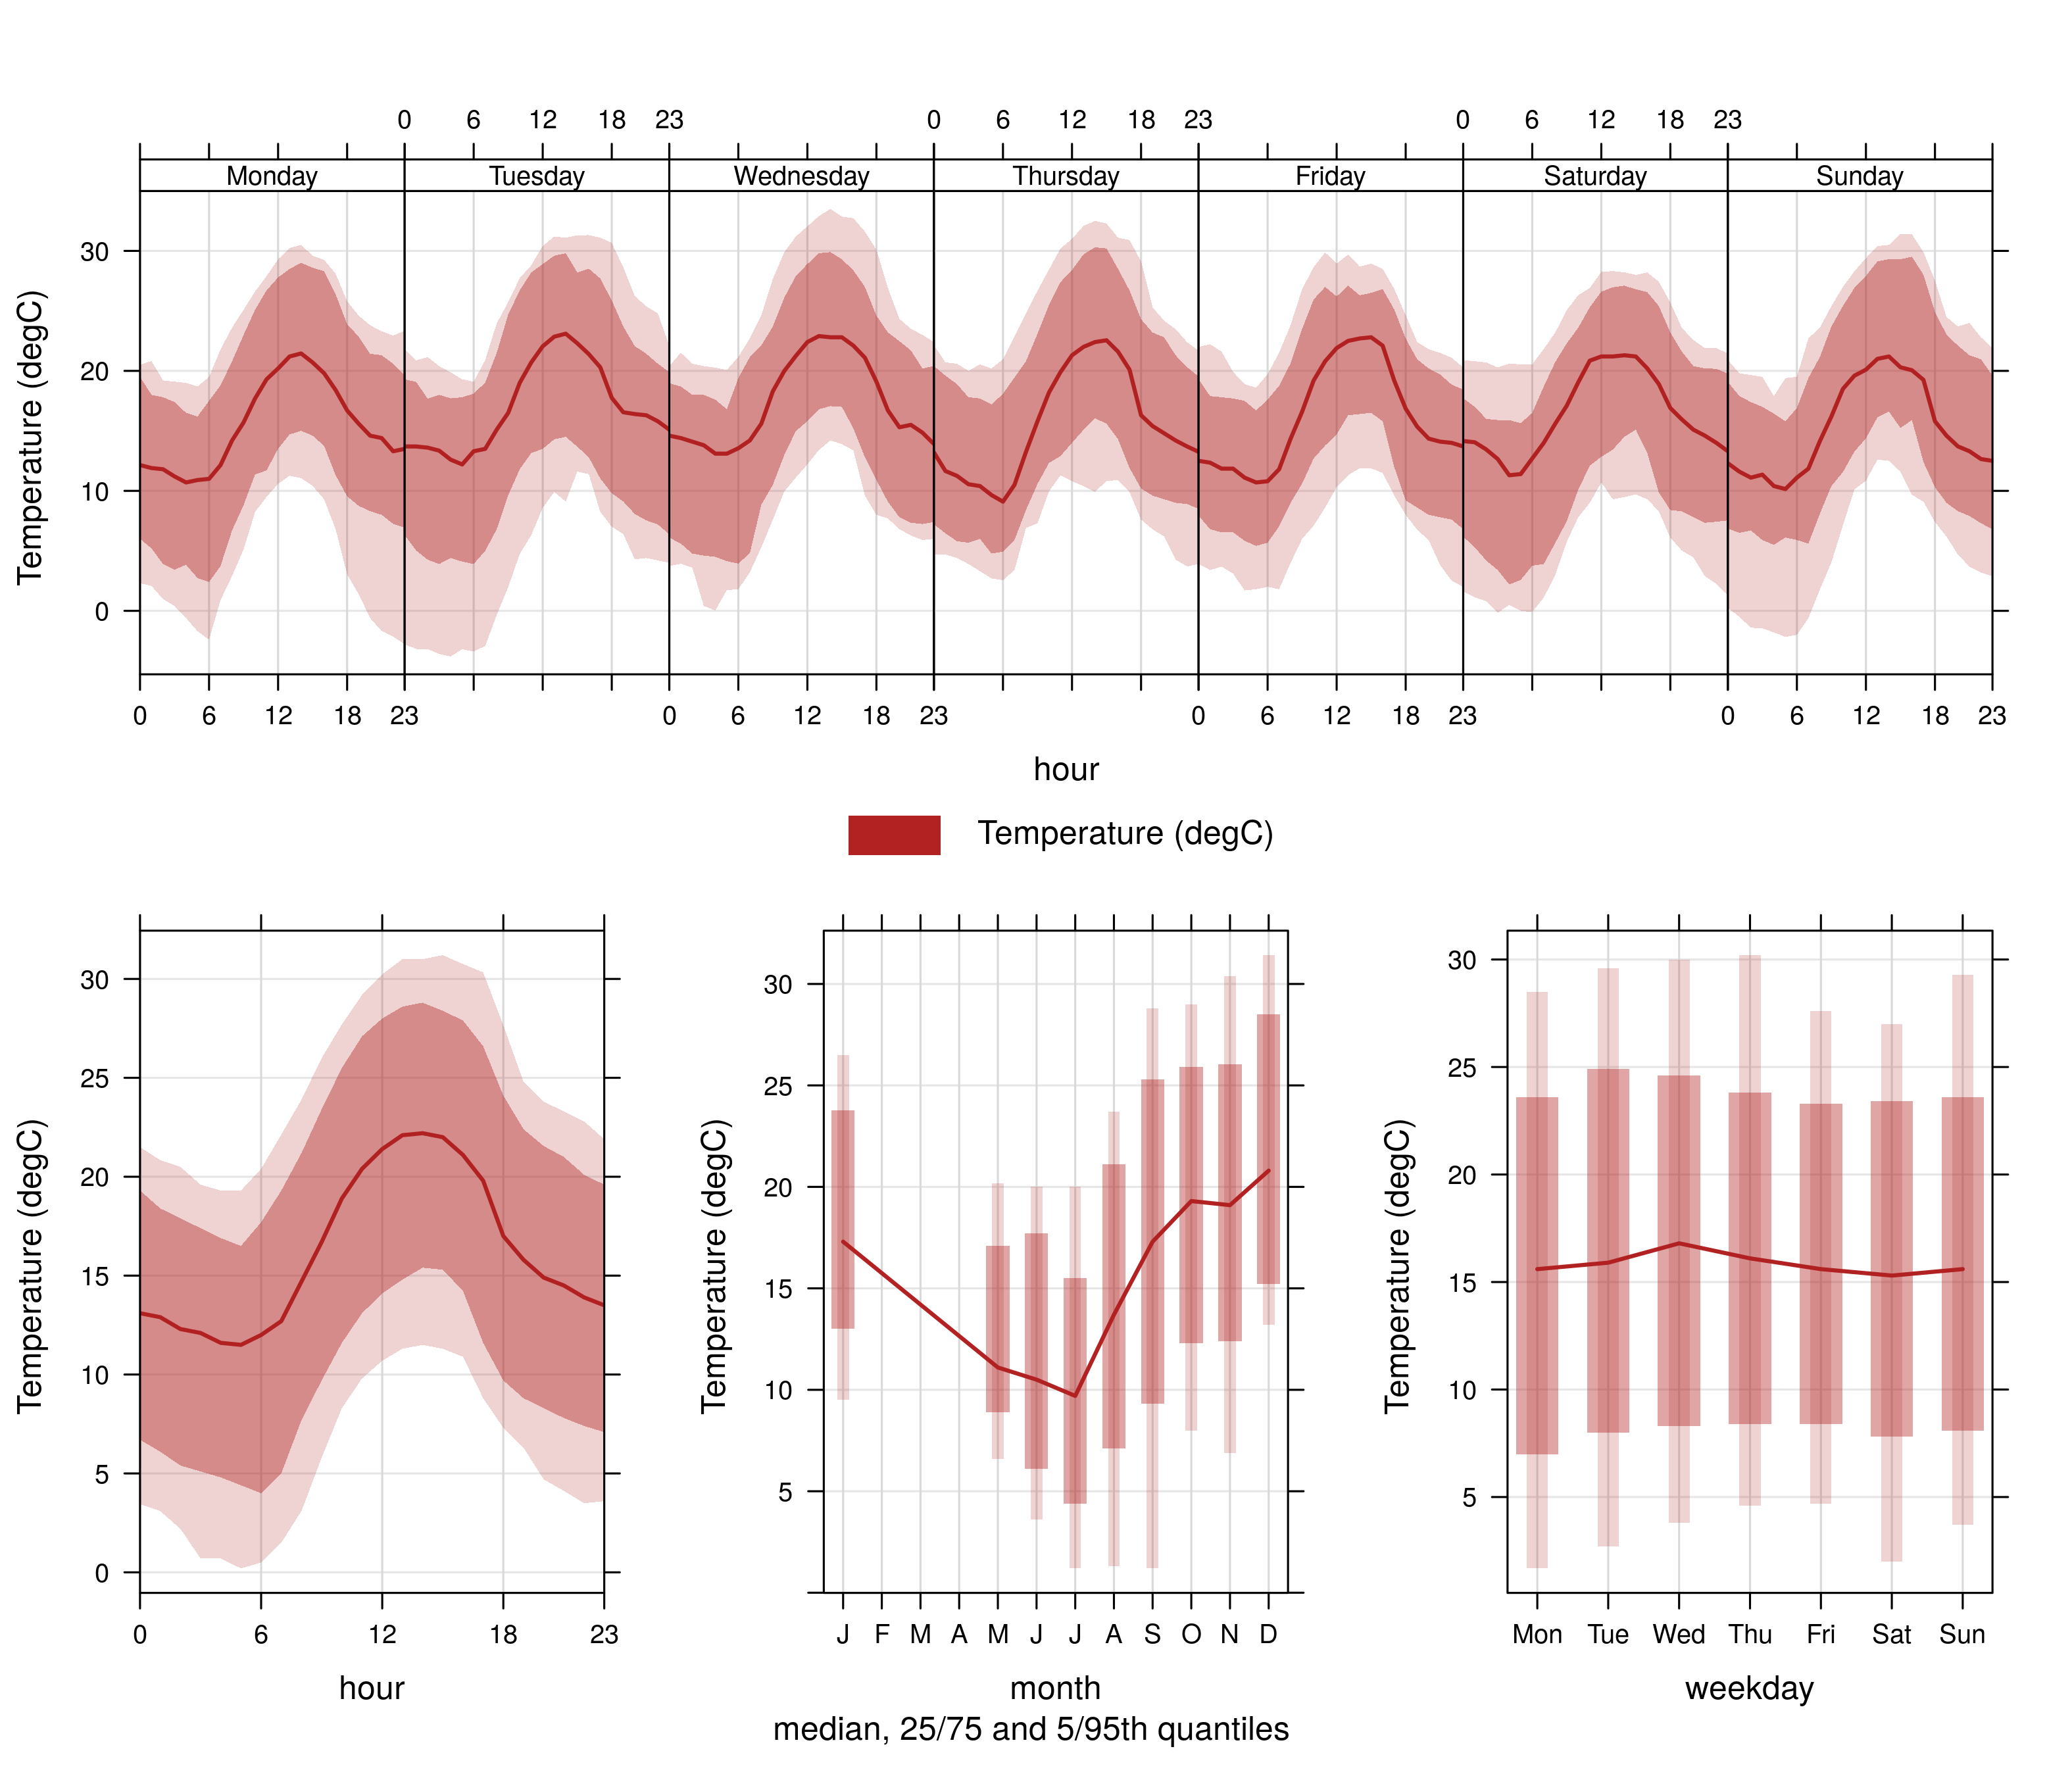
\includegraphics[width=\textwidth]{images/Wedela_Temperature_timevary.png}
    \caption[Time variation of temperature measurements at Wedela.]{Time variation of temperature measurements at Wedela.}
    \label{fig:summary-tmp}
\end{figure}

\begin{figure}[!htb]
    \centering
    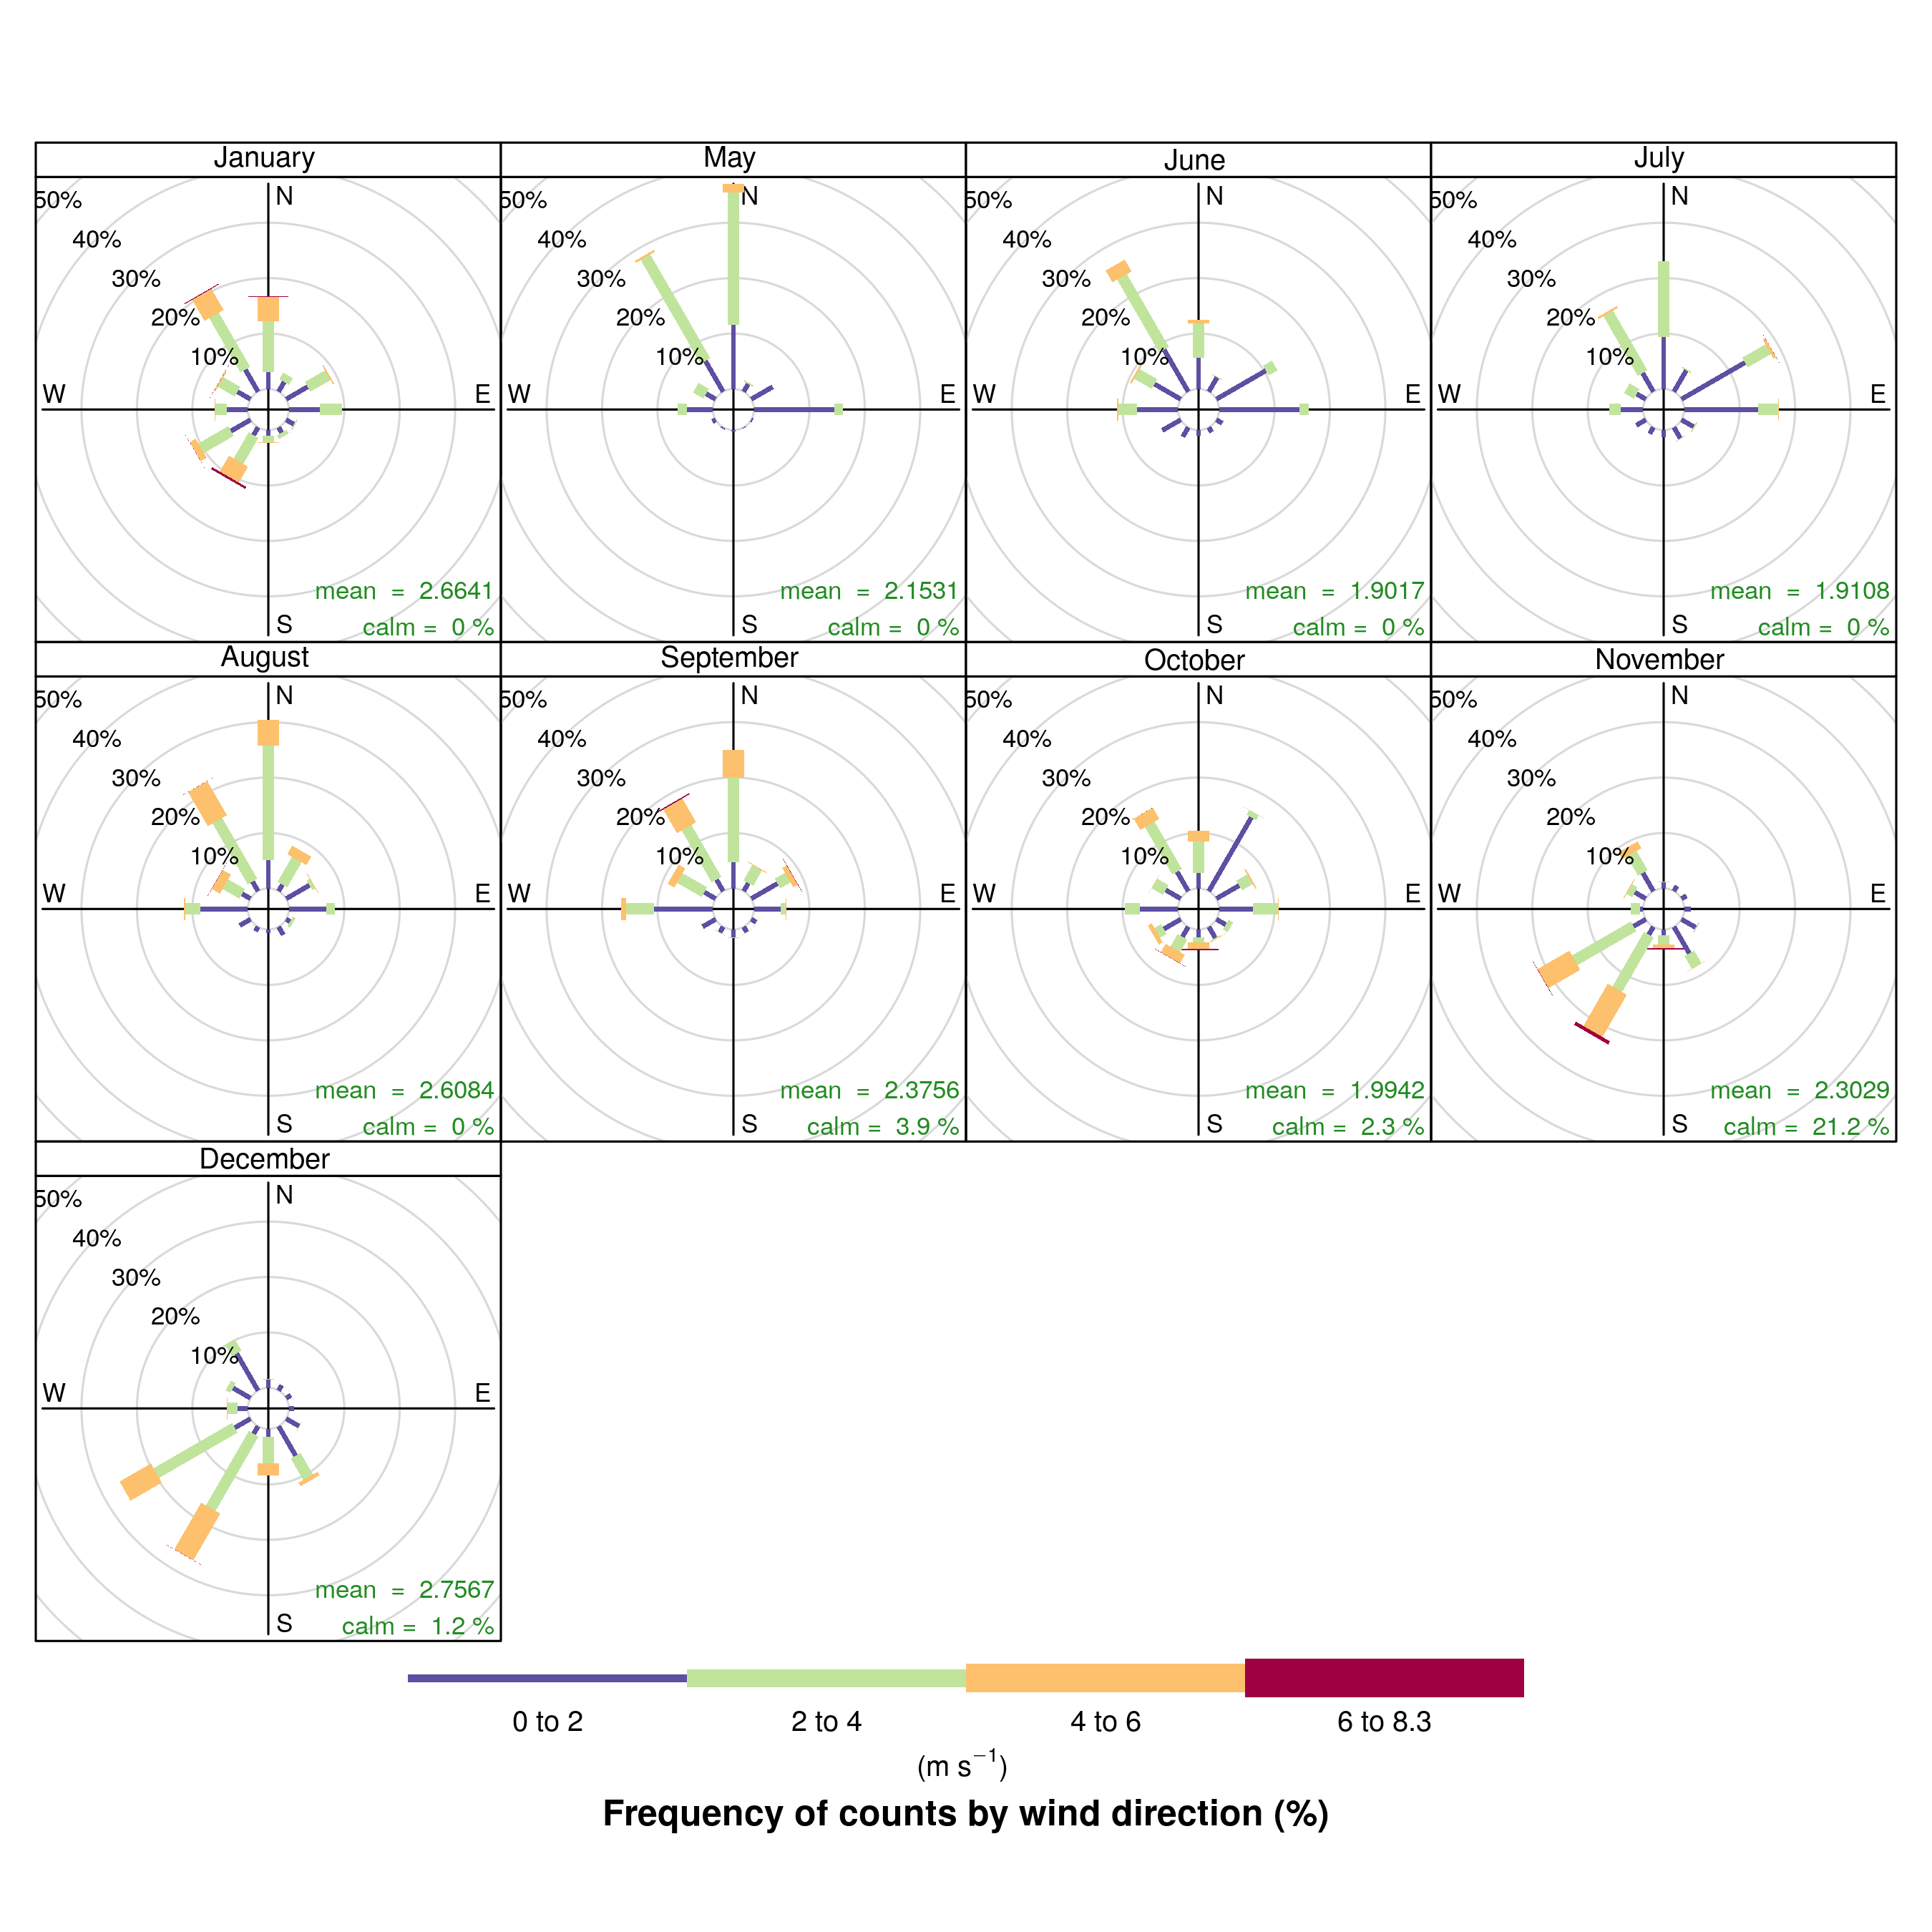
\includegraphics[width=\textwidth]{images/Wedela-windrose-monthly.png}
    \caption[Monthly wind roses at Wedela.]{Monthly wind roses during the sampling period for Wedela.}
    \label{fig:windrose-monthly}
\end{figure}

\begin{figure}[!htb]
    \centering
    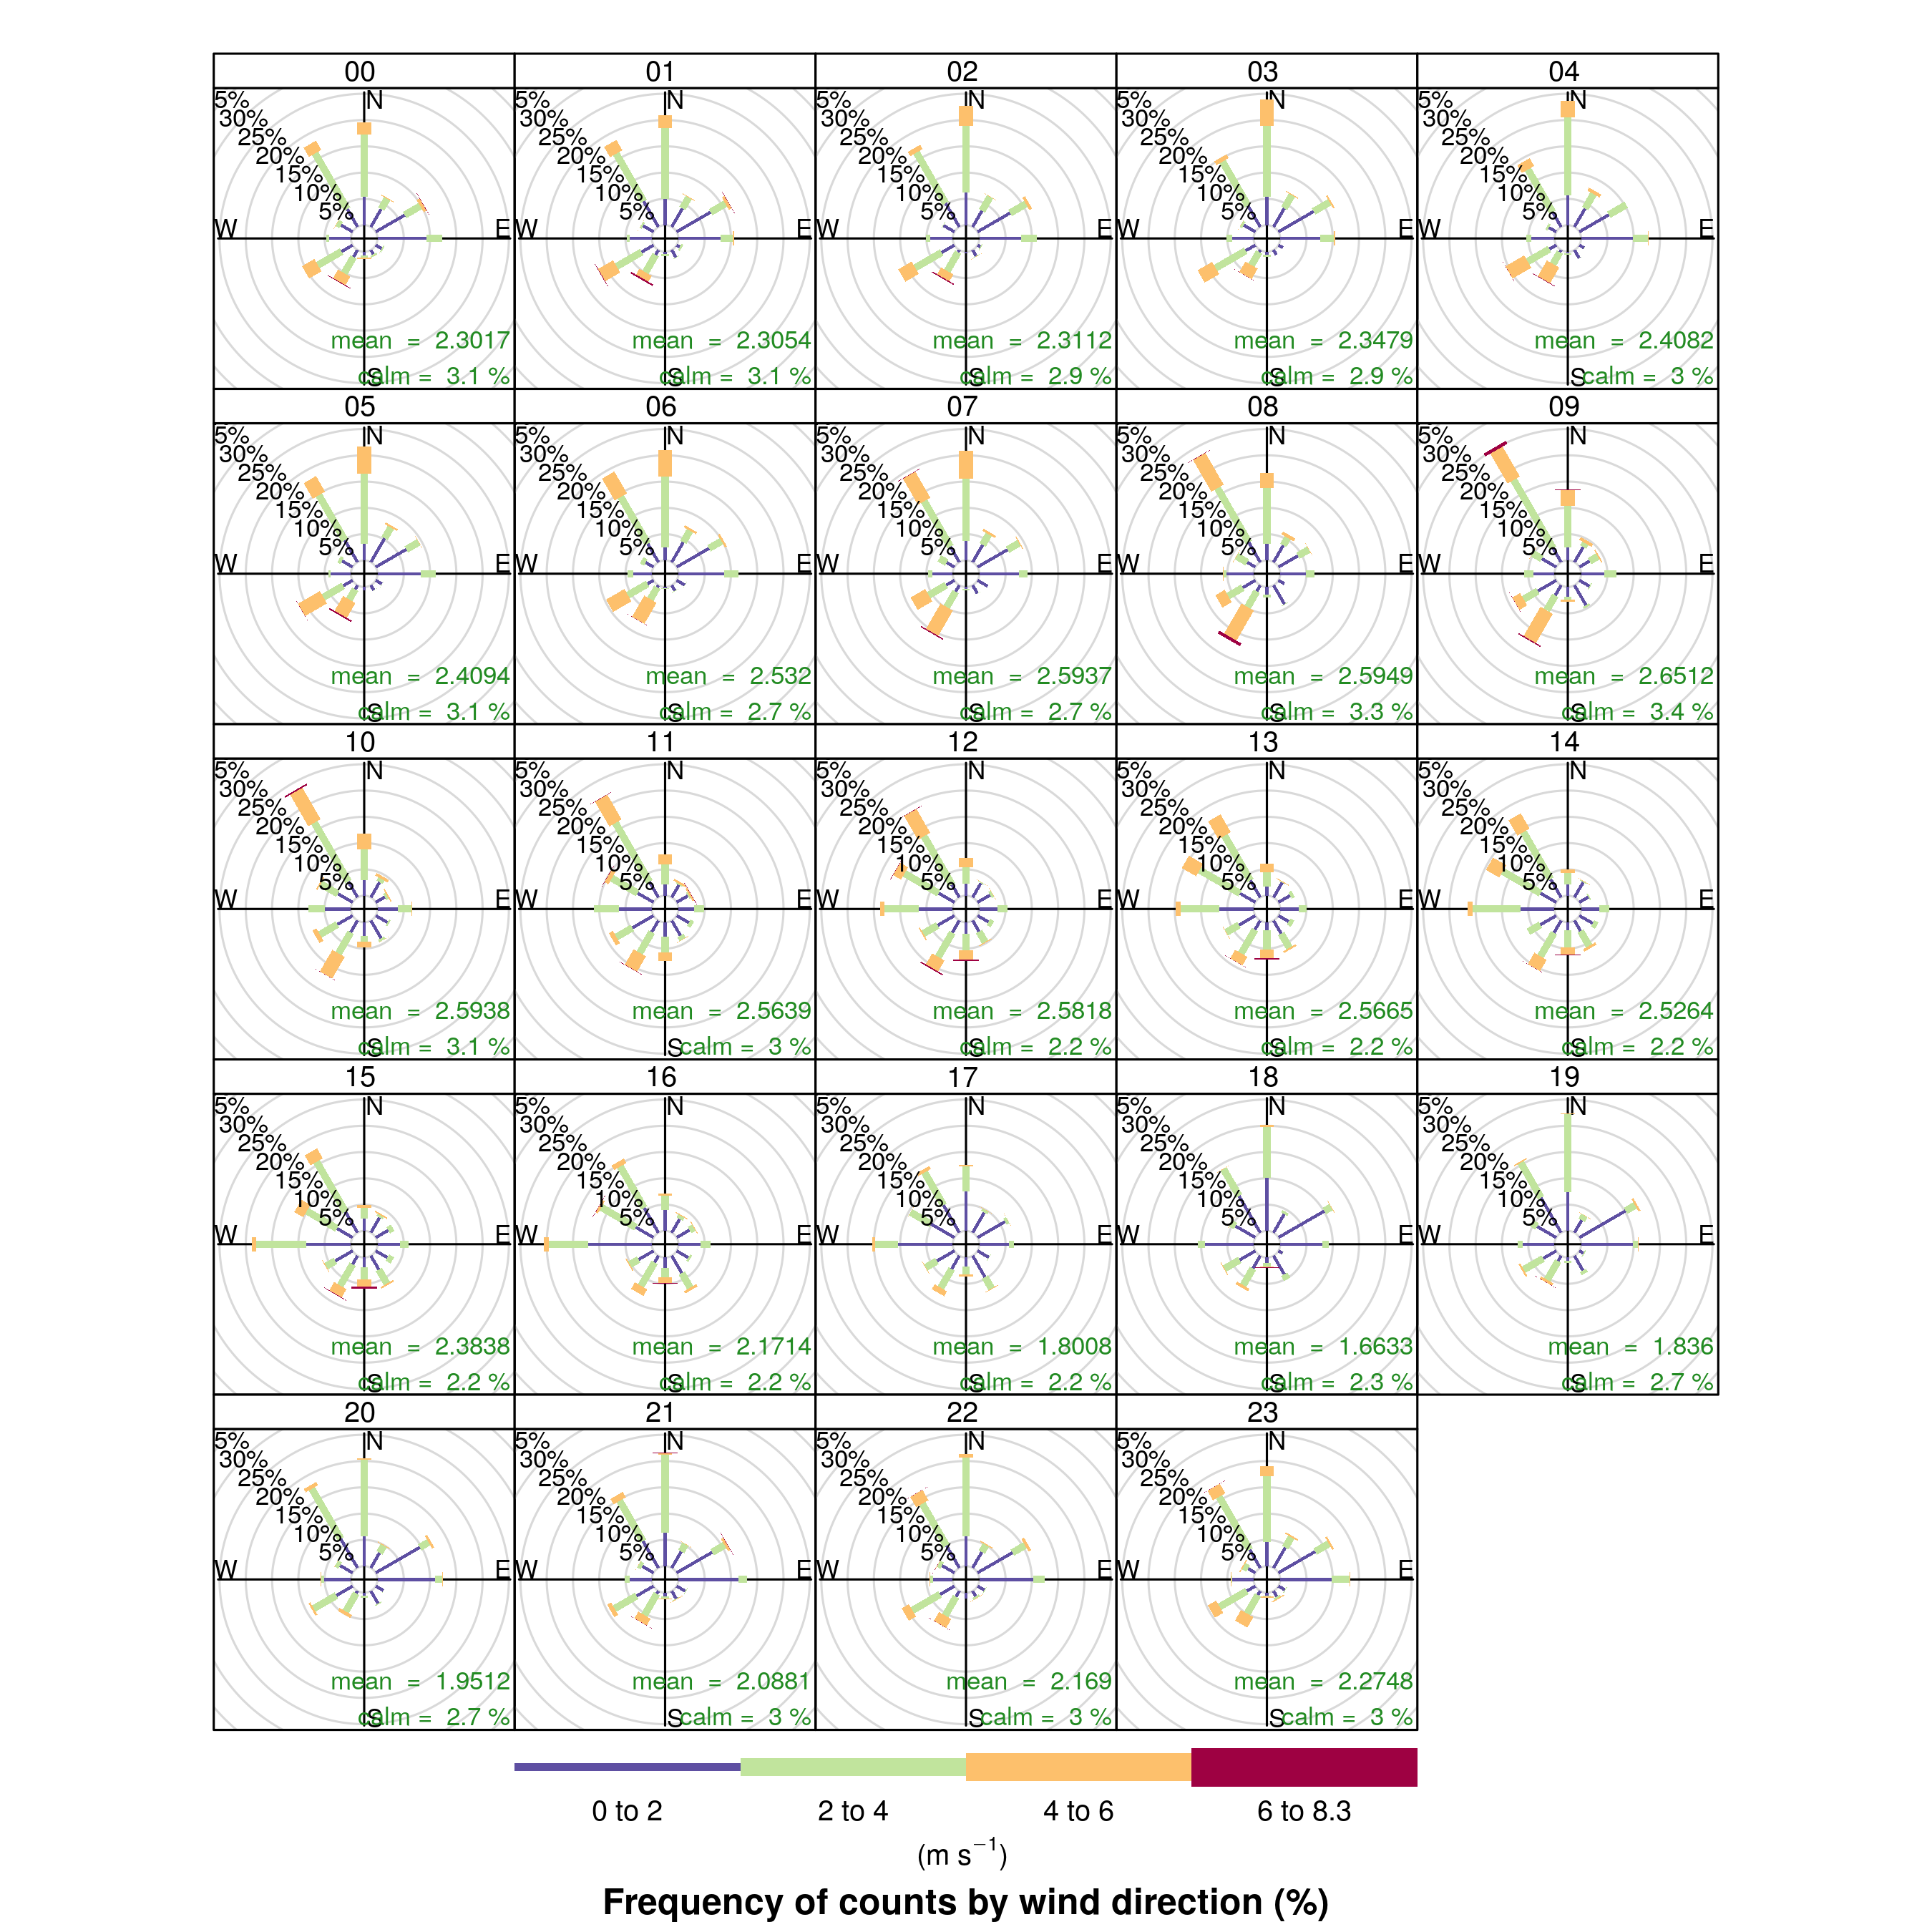
\includegraphics[width=\textwidth]{images/Wedela-windrose-hourly.png}
    \caption[Hourly wind roses for Wedela]{Hourly wind roses during the sampling period for Wedela}
    \label{fig:windrose-hourly}
\end{figure}

\begin{figure}[!htb]
    \centering
    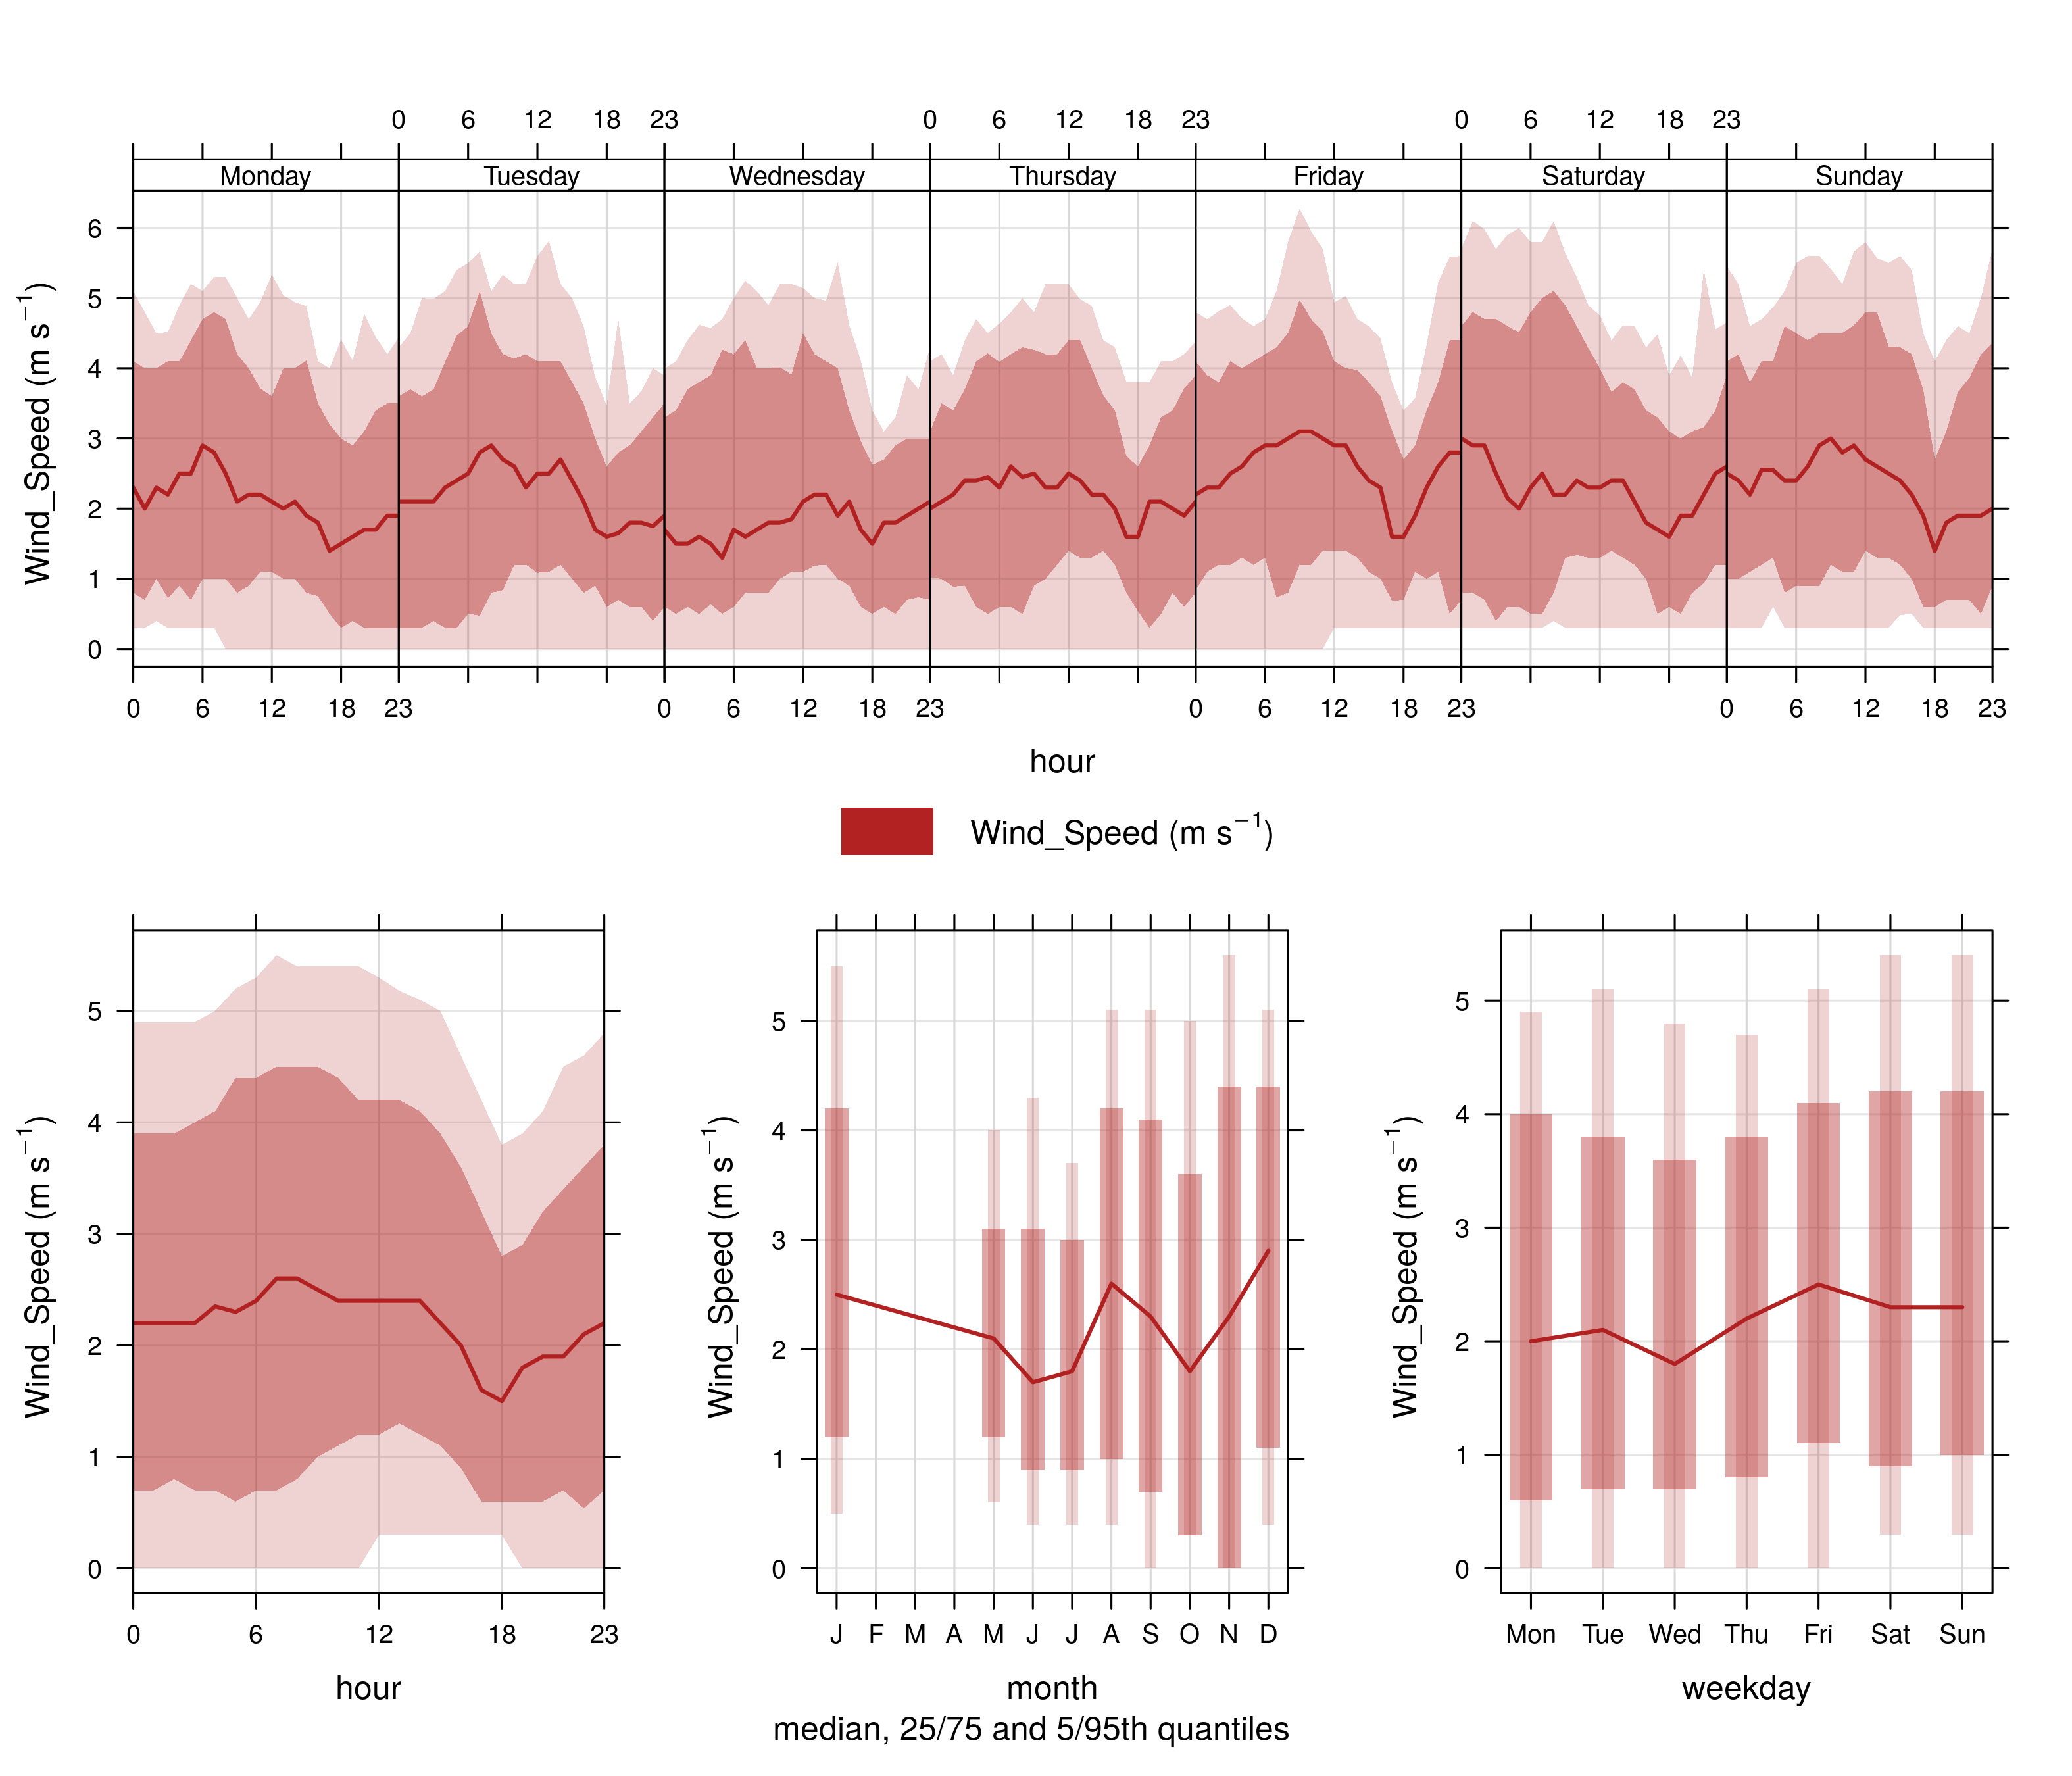
\includegraphics[width=\textwidth]{images/Wedela_Wind_Speed_timevary.png}
    \caption{Time variation of wind speed in Wedela.}
    \label{fig:timevary-winds}
\end{figure}

\section{Measurements of atmospheric particulate matter}

\gls{pm} comprises a mixture of solid and/or liquid particles (organic and inorganic) suspended in air. Even though \gls{pm} is a widespread pollutant, the chemical and physical characteristics of the \gls{pm} mixture may vary greatly by location and source. The fact that \gls{pm} could be formed primarily or secondarily and continues to undergo chemical and physical transformation whilst in the atmosphere, further adds to its complexity. This variability complicates the study of exposure and risks as different characteristics of \gls{pm} may cause different health effects (Samet et al., 2006). There is currently not enough evidence at the population level to conclusively determine the effects of different chemical compositions or sources of \gls{pm} on health (WHO, 2006). For this reason, air quality guidelines still classify particles by their aerodynamic properties. This is still the most widely used method of classification since the aerodynamic properties of particulates influence their transport and removal from the atmosphere in addition to their deposition sites and clearance pathways in the respiratory system (WHO, 2006).

A summary of the data collected is presented in Table~\ref{table:pmstats}.

\begin{table}[!htbp]
\caption[Statistics for ambient particulate matter during
the campaign.]{Statistics for ambient particulate matter measurements between June 2018 and January 2019. The exceedances are measured against the daily average \gls{pm2.5} standard of \SI{40}{\micro\gram\per\cubic\meter} and \SI{75}{\micro\gram\per\cubic\meter} for \gls{pm10}}
\label{table:pmstats}
\begin{center}
\begin{tabular}{lrrrrrrrrrrrrr}
\toprule
\textbf{Month}& \rotatebox[origin=c]{90}{\textbf{Average}}& \textbf{Interval}& \textbf{N}& \rotatebox[origin=c]{90}{\textbf{Exceedances}}& \rotatebox[origin=c]{90}{\textbf{Std Dev}}& \rotatebox[origin=c]{90}{\textbf{Median}}& \textbf{\SI{25}{\percent}}& \textbf{\SI{75}{\percent}}& \textbf{\SI{99}{\percent}}& \rotatebox[origin=c]{90}{\textbf{Available (\%)}} \\
\midrule
\multicolumn{11}{l}{\bfseries \textbf{\gls{pm2.5} (\si{\micro\gram\per\cubic\meter})}} \\
Jul &  13 &  10-16 &  27 &  0 &   6 &  12 &   9 &  15 &  31 &  87 \\
Aug &  18 &  14-21 &  27 &  0 &   7 &  19 &  12 &  22 &   32 &  87 \\
Sep &  30 &  21-39 &  14 &  3 &  11 &  29 &  24 &  32 &   56 &  47 \\
Oct &  13 &  11-16 &  28 &  0 &   5 &  14 &  11 &  17 &  20 &  90 \\
Nov &  12 &   9-15 &  18 &  0 &   4 &  12 &   9 &  15 &  22 &  60 \\
Dec &   7 &    6-9 &  21 &  0 &  2 &   8 &   6 &   9 &  11 &  68 \\
Jan &   9 &   7-11 &  28 &  0 &  4 &   8 &   6 &  11 &  17 &  90 \\
\midrule
\multicolumn{11}{l}{\bfseries \textbf{\gls{pm10} (\si{\micro\gram\per\cubic\meter})}} \\
Jul &  32 &  25-39 &  27 &  0 &  13 &  30 &  24 &  33 &  62 &  87 \\
Aug &  55 &  39-71 &  28 &  4 &  30 &  50 &  38 &  61 &  146 &  90 \\
Sep &  61 &  40-81 &  15 &  5 &  27 &  56 &  41 &  80 &  109 &  50 \\
Oct &  32 &  19-44 &  16 &  0 &  17 &  28 &  18 &  39 &  70 &  52 \\
Nov &  35 &  28-42 &  18 &  0 &  10 &  33 &  29 &  42 &  54 &  60 \\
Dec &  19 &  16-22 &  17 &  0 &  4 &  20 &  16 &  21 &  26 &  55 \\
Jan &  13 &  8-19 &   9 &  0 &  5 &  13 &  11 &  14 &  23 &  29 \\
\bottomrule

\end{tabular}
\end{center}
\end{table}

\begin{figure}[!htb]
    \centering
    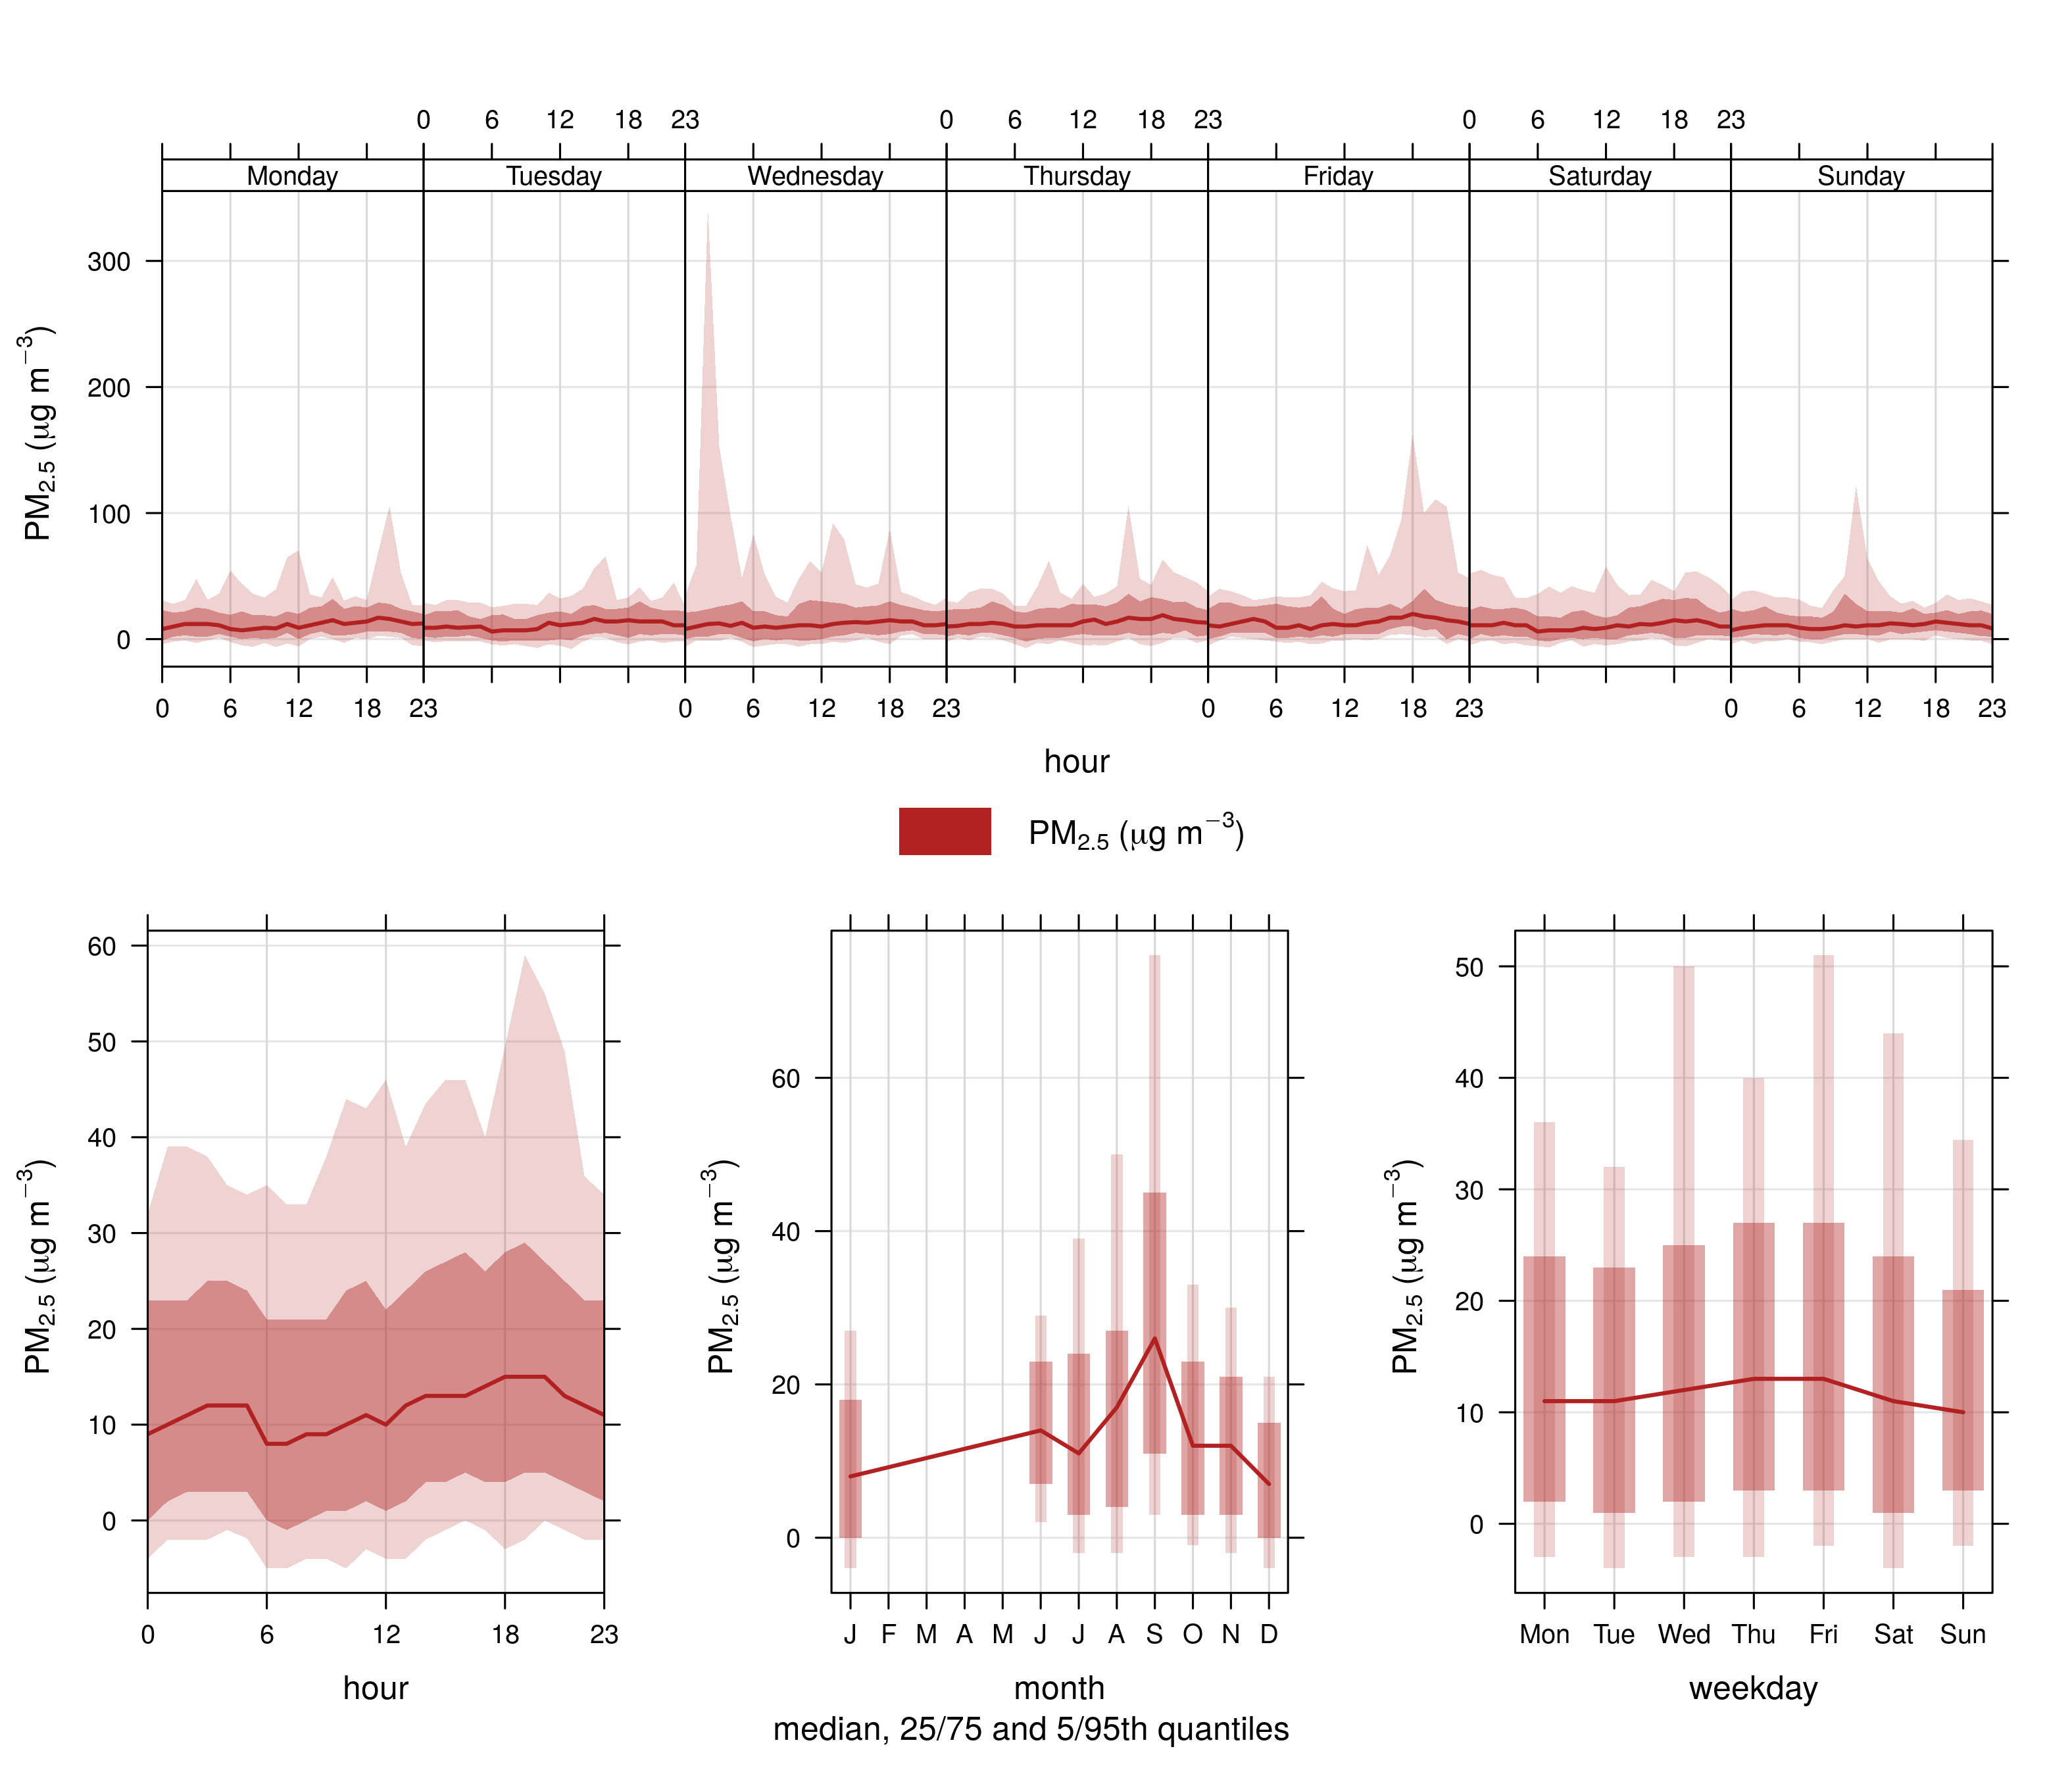
\includegraphics[width=\textwidth]{images/Wedela_PM2-5_timevary.png}
    \caption[The variability of $PM_{2.5}$ with time.]{The variability of \gls{pm2.5} with time.}
    \label{fig:summary}
\end{figure}

\begin{figure}[!htb]
    \centering
    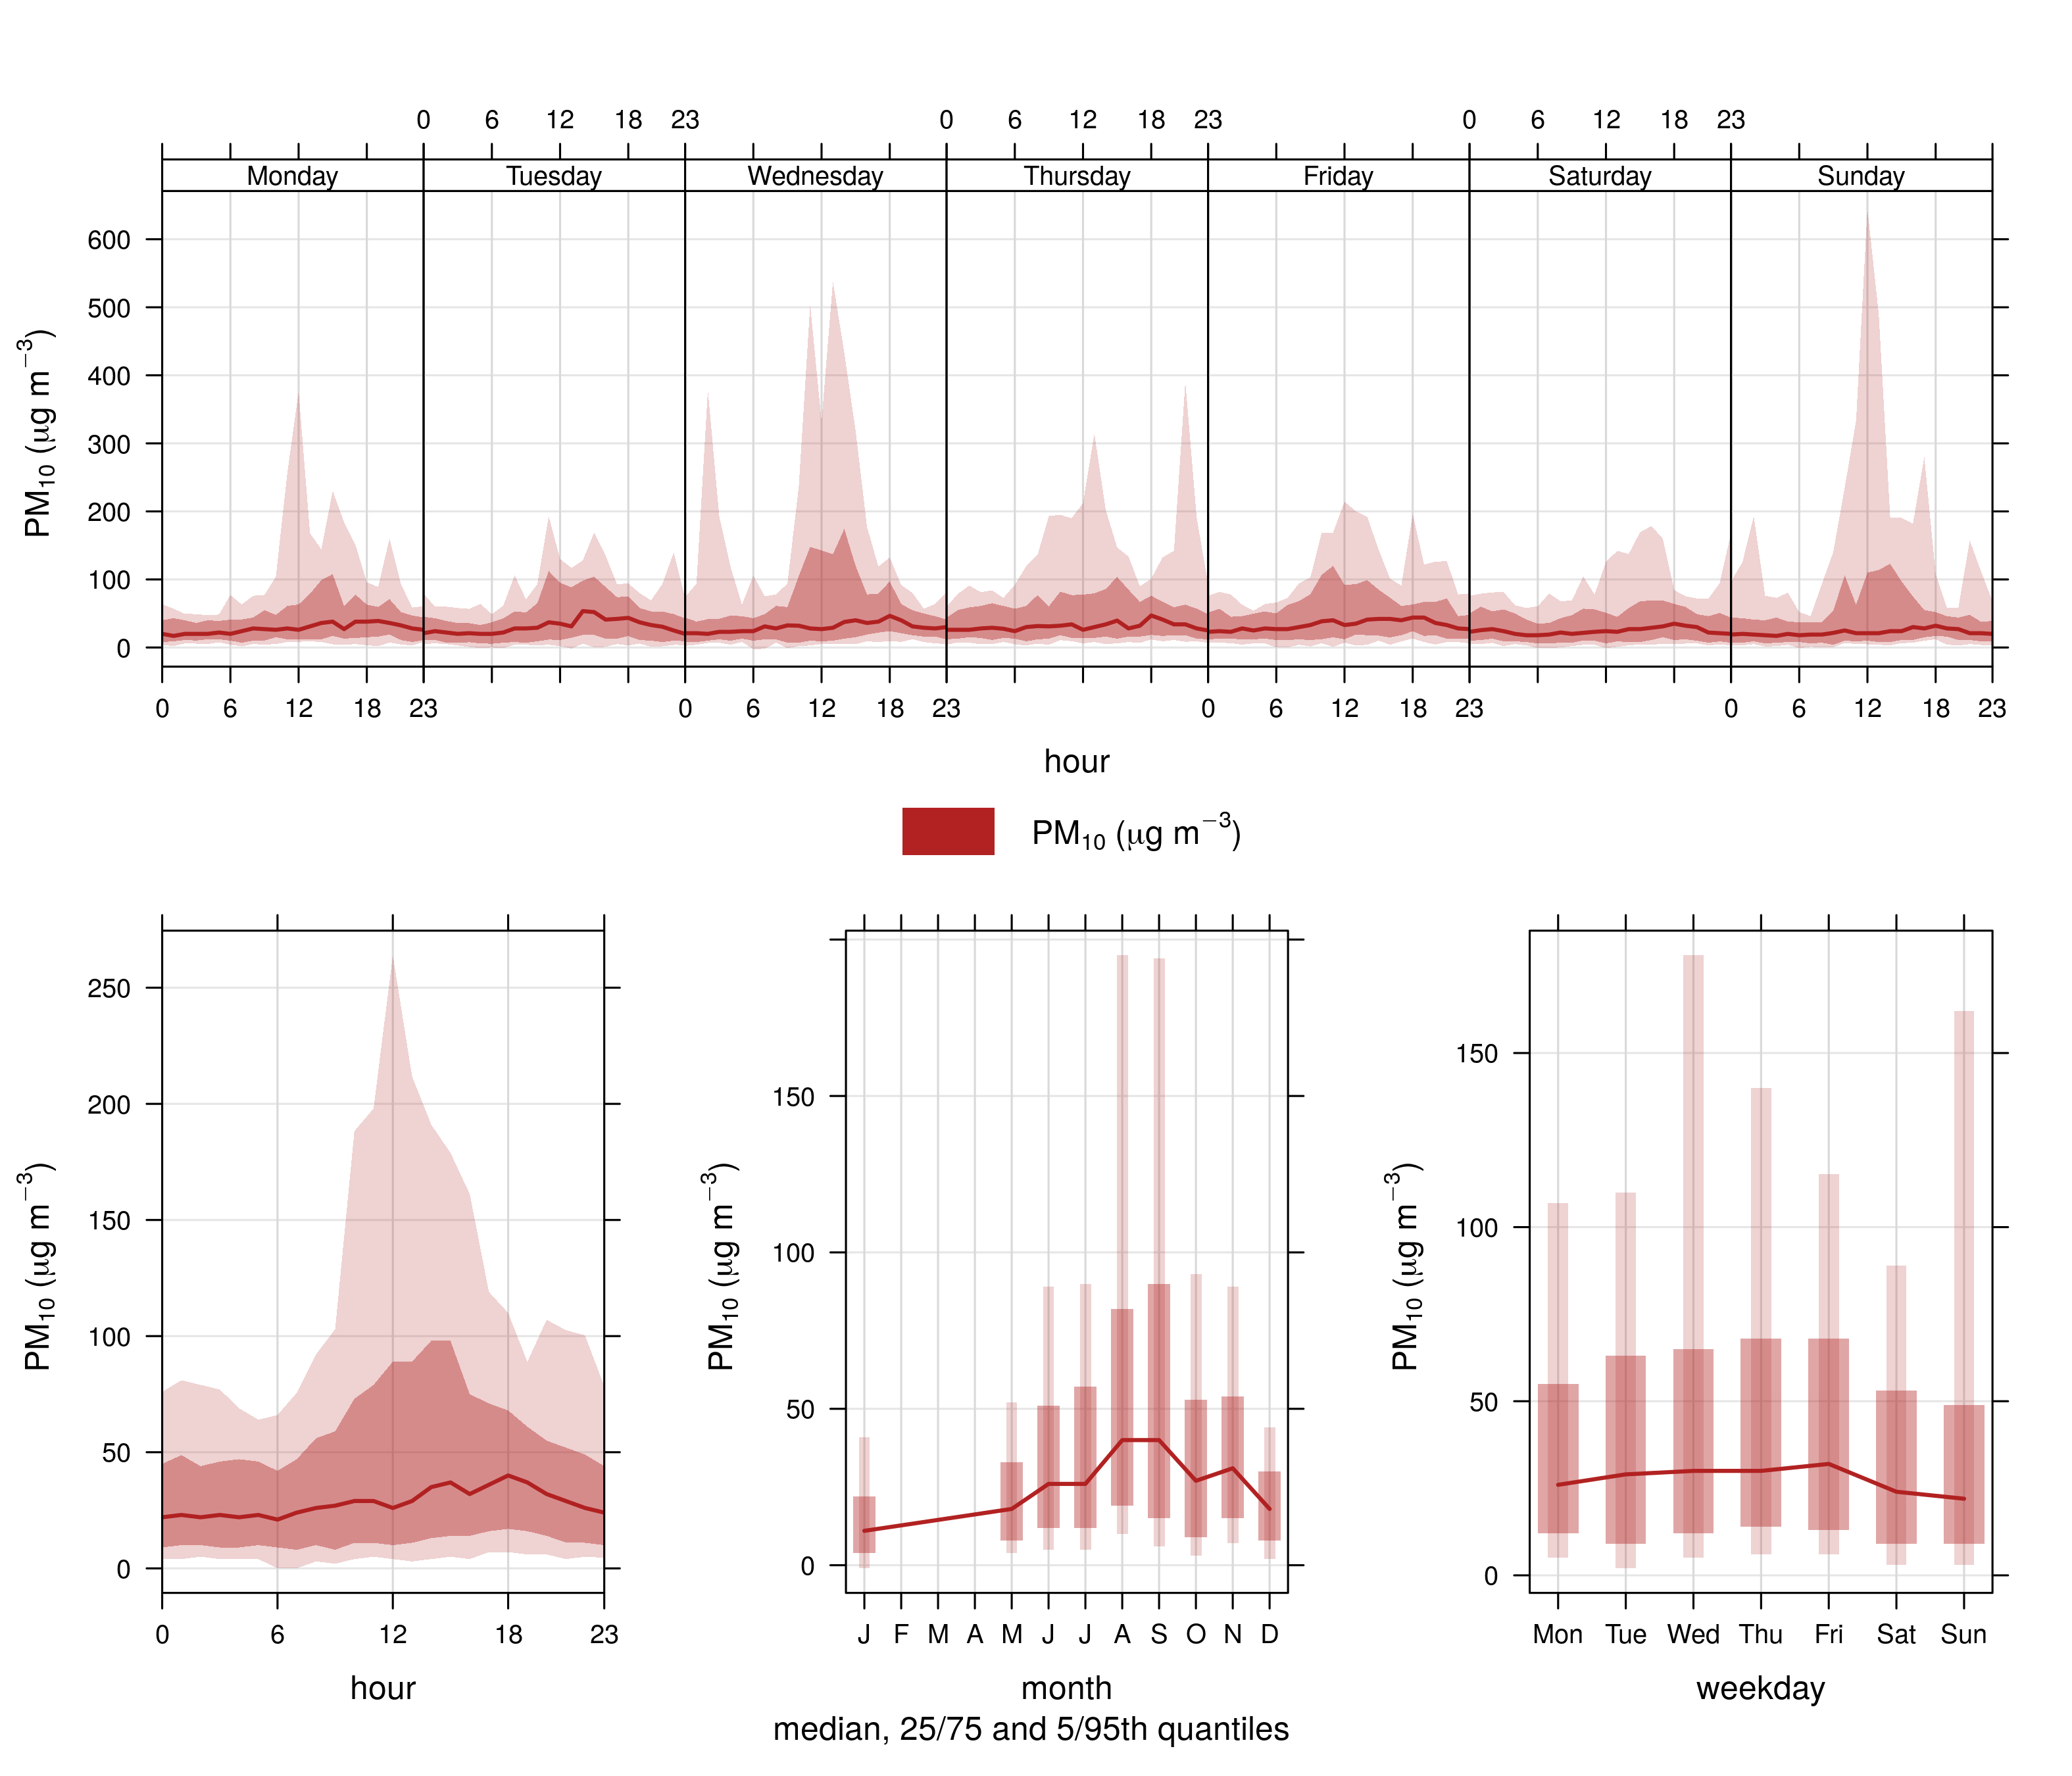
\includegraphics[width=\textwidth]{images/Wedela_PM10_timevary.png}
    \caption[The variability of $PM_{10}$ with time.]{The variability of \gls{pm10} with time.}
    \label{fig:summary}
\end{figure}

\begin{figure}[!htb]
    \centering
    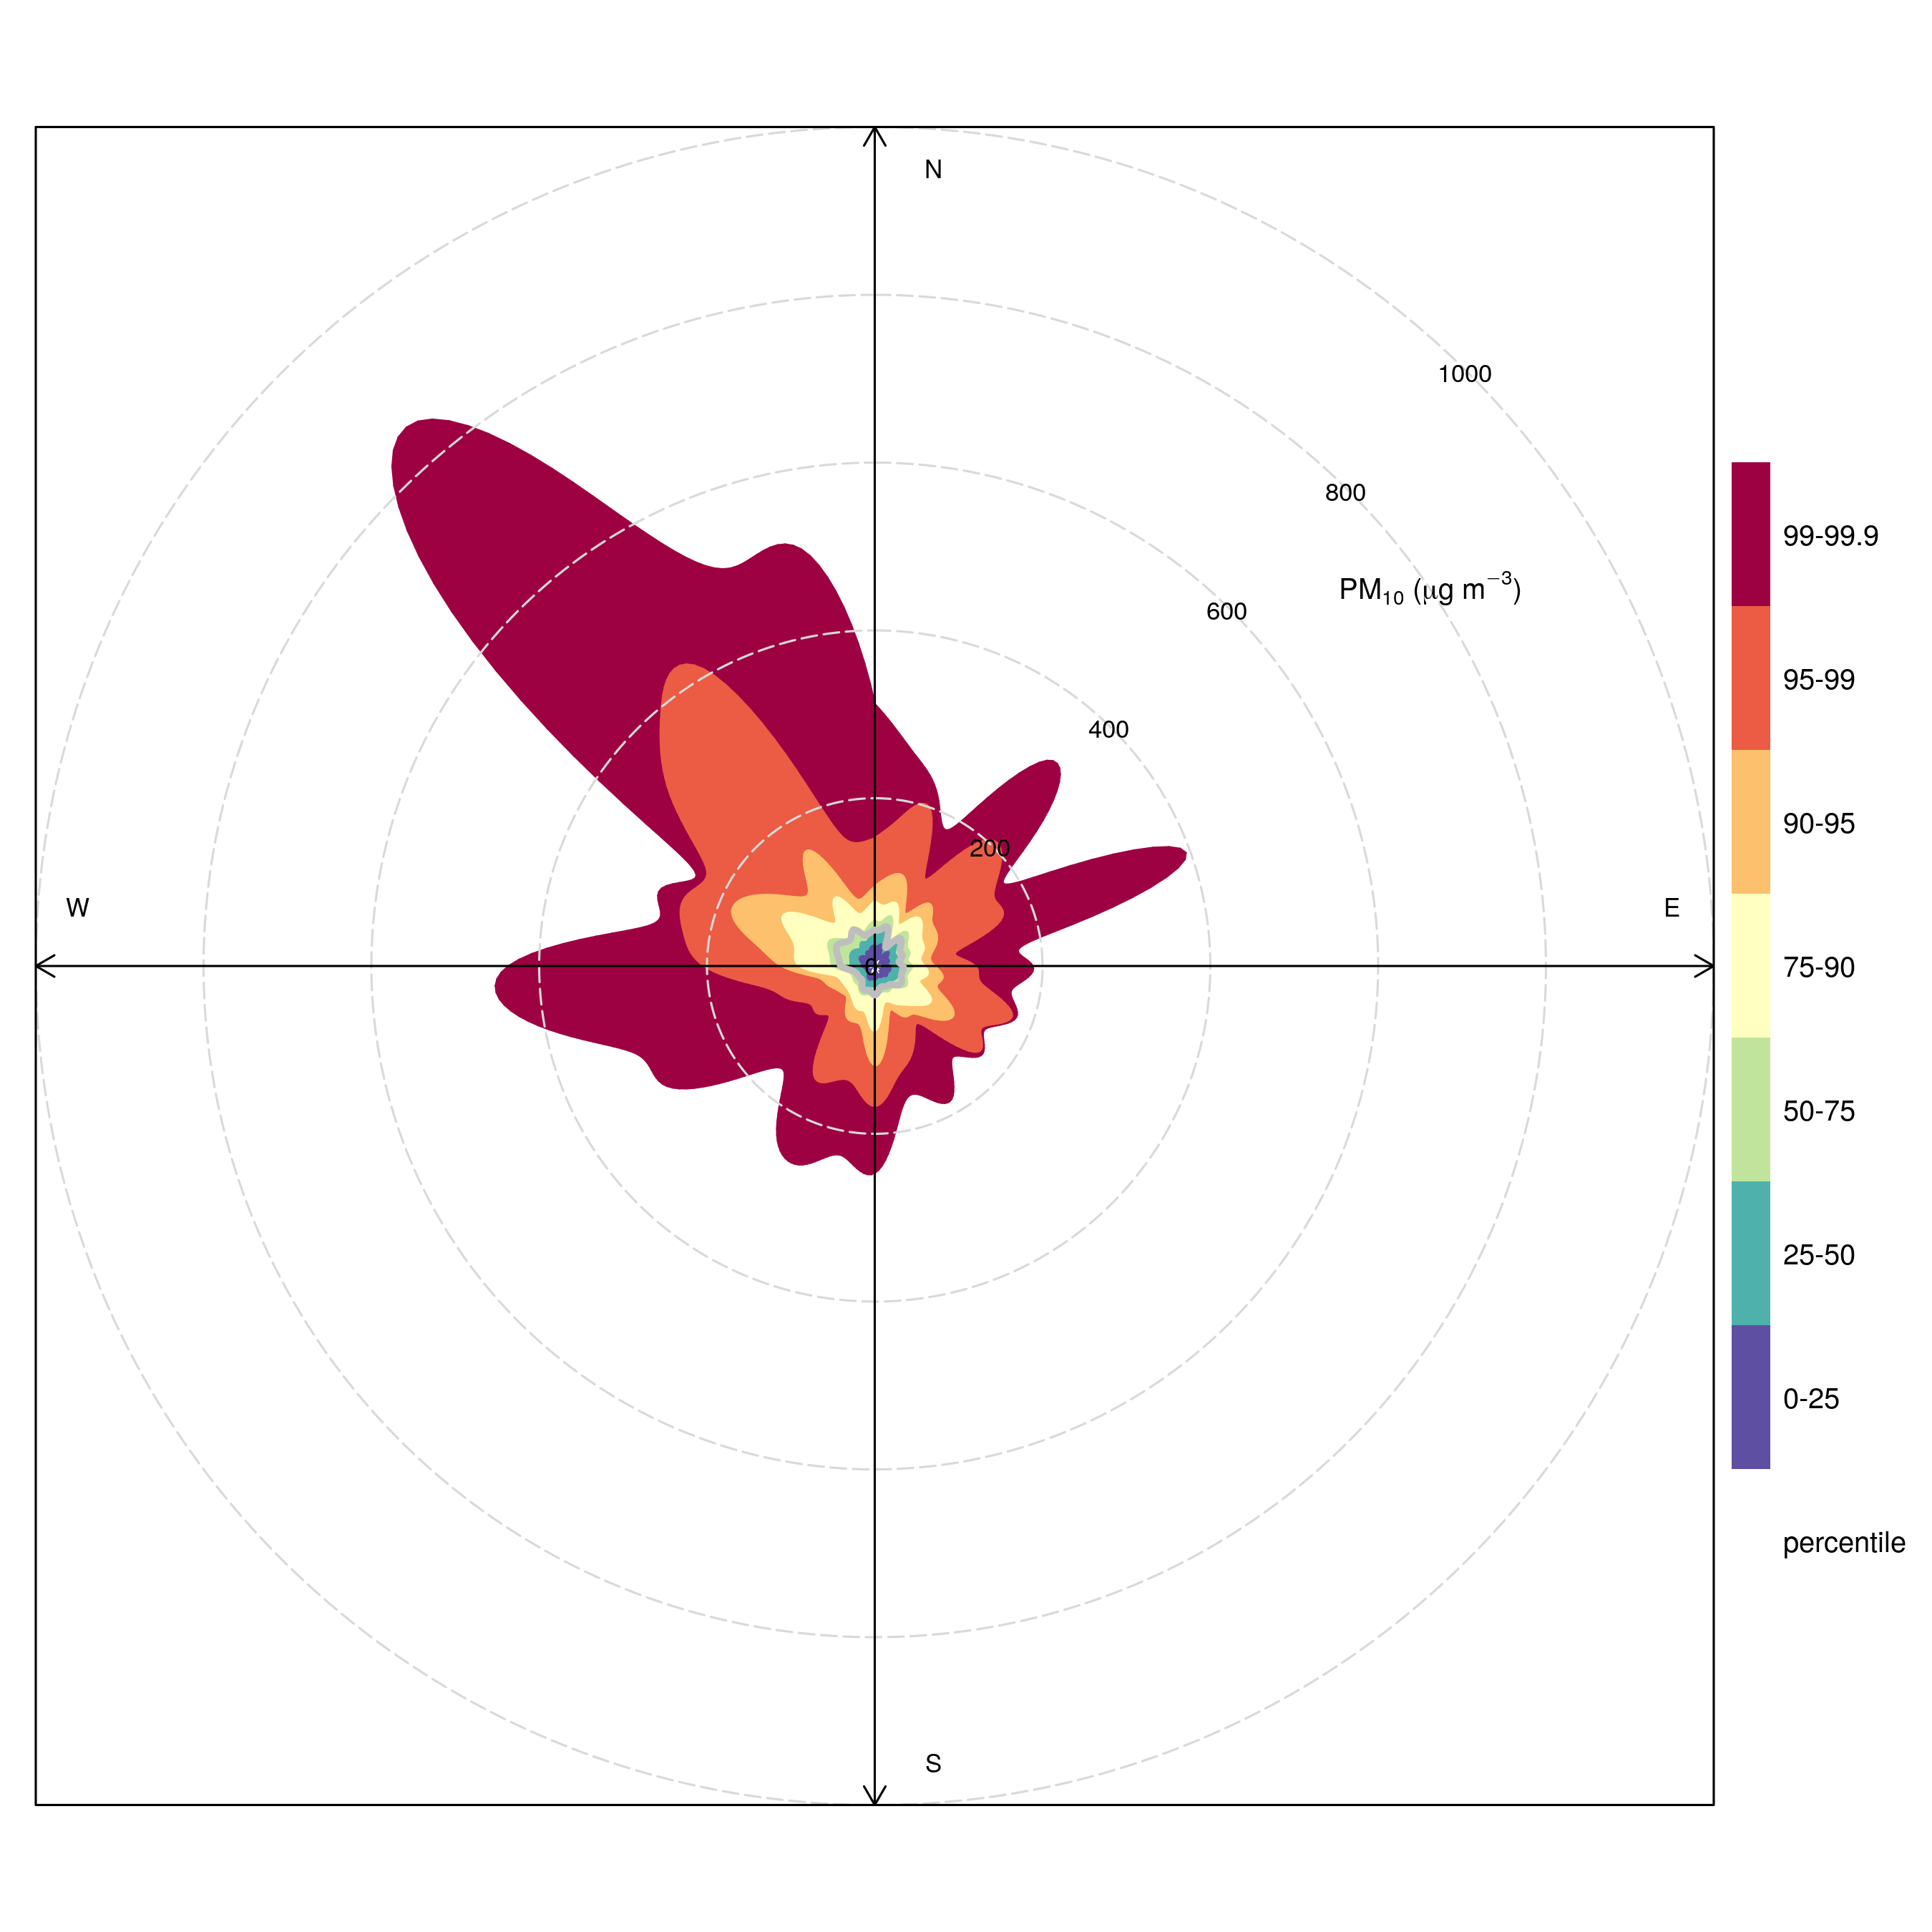
\includegraphics[width=\textwidth]{images/Wedela_PM10_percentileRose.png}
    \caption[Pollution rose for $PM_{10}$ for the sampling campaign.]{Pollution rose for \gls{pm10} for the sampling campaign.}
    \label{fig:summary}
\end{figure}

\begin{figure}[!htb]
    \centering
    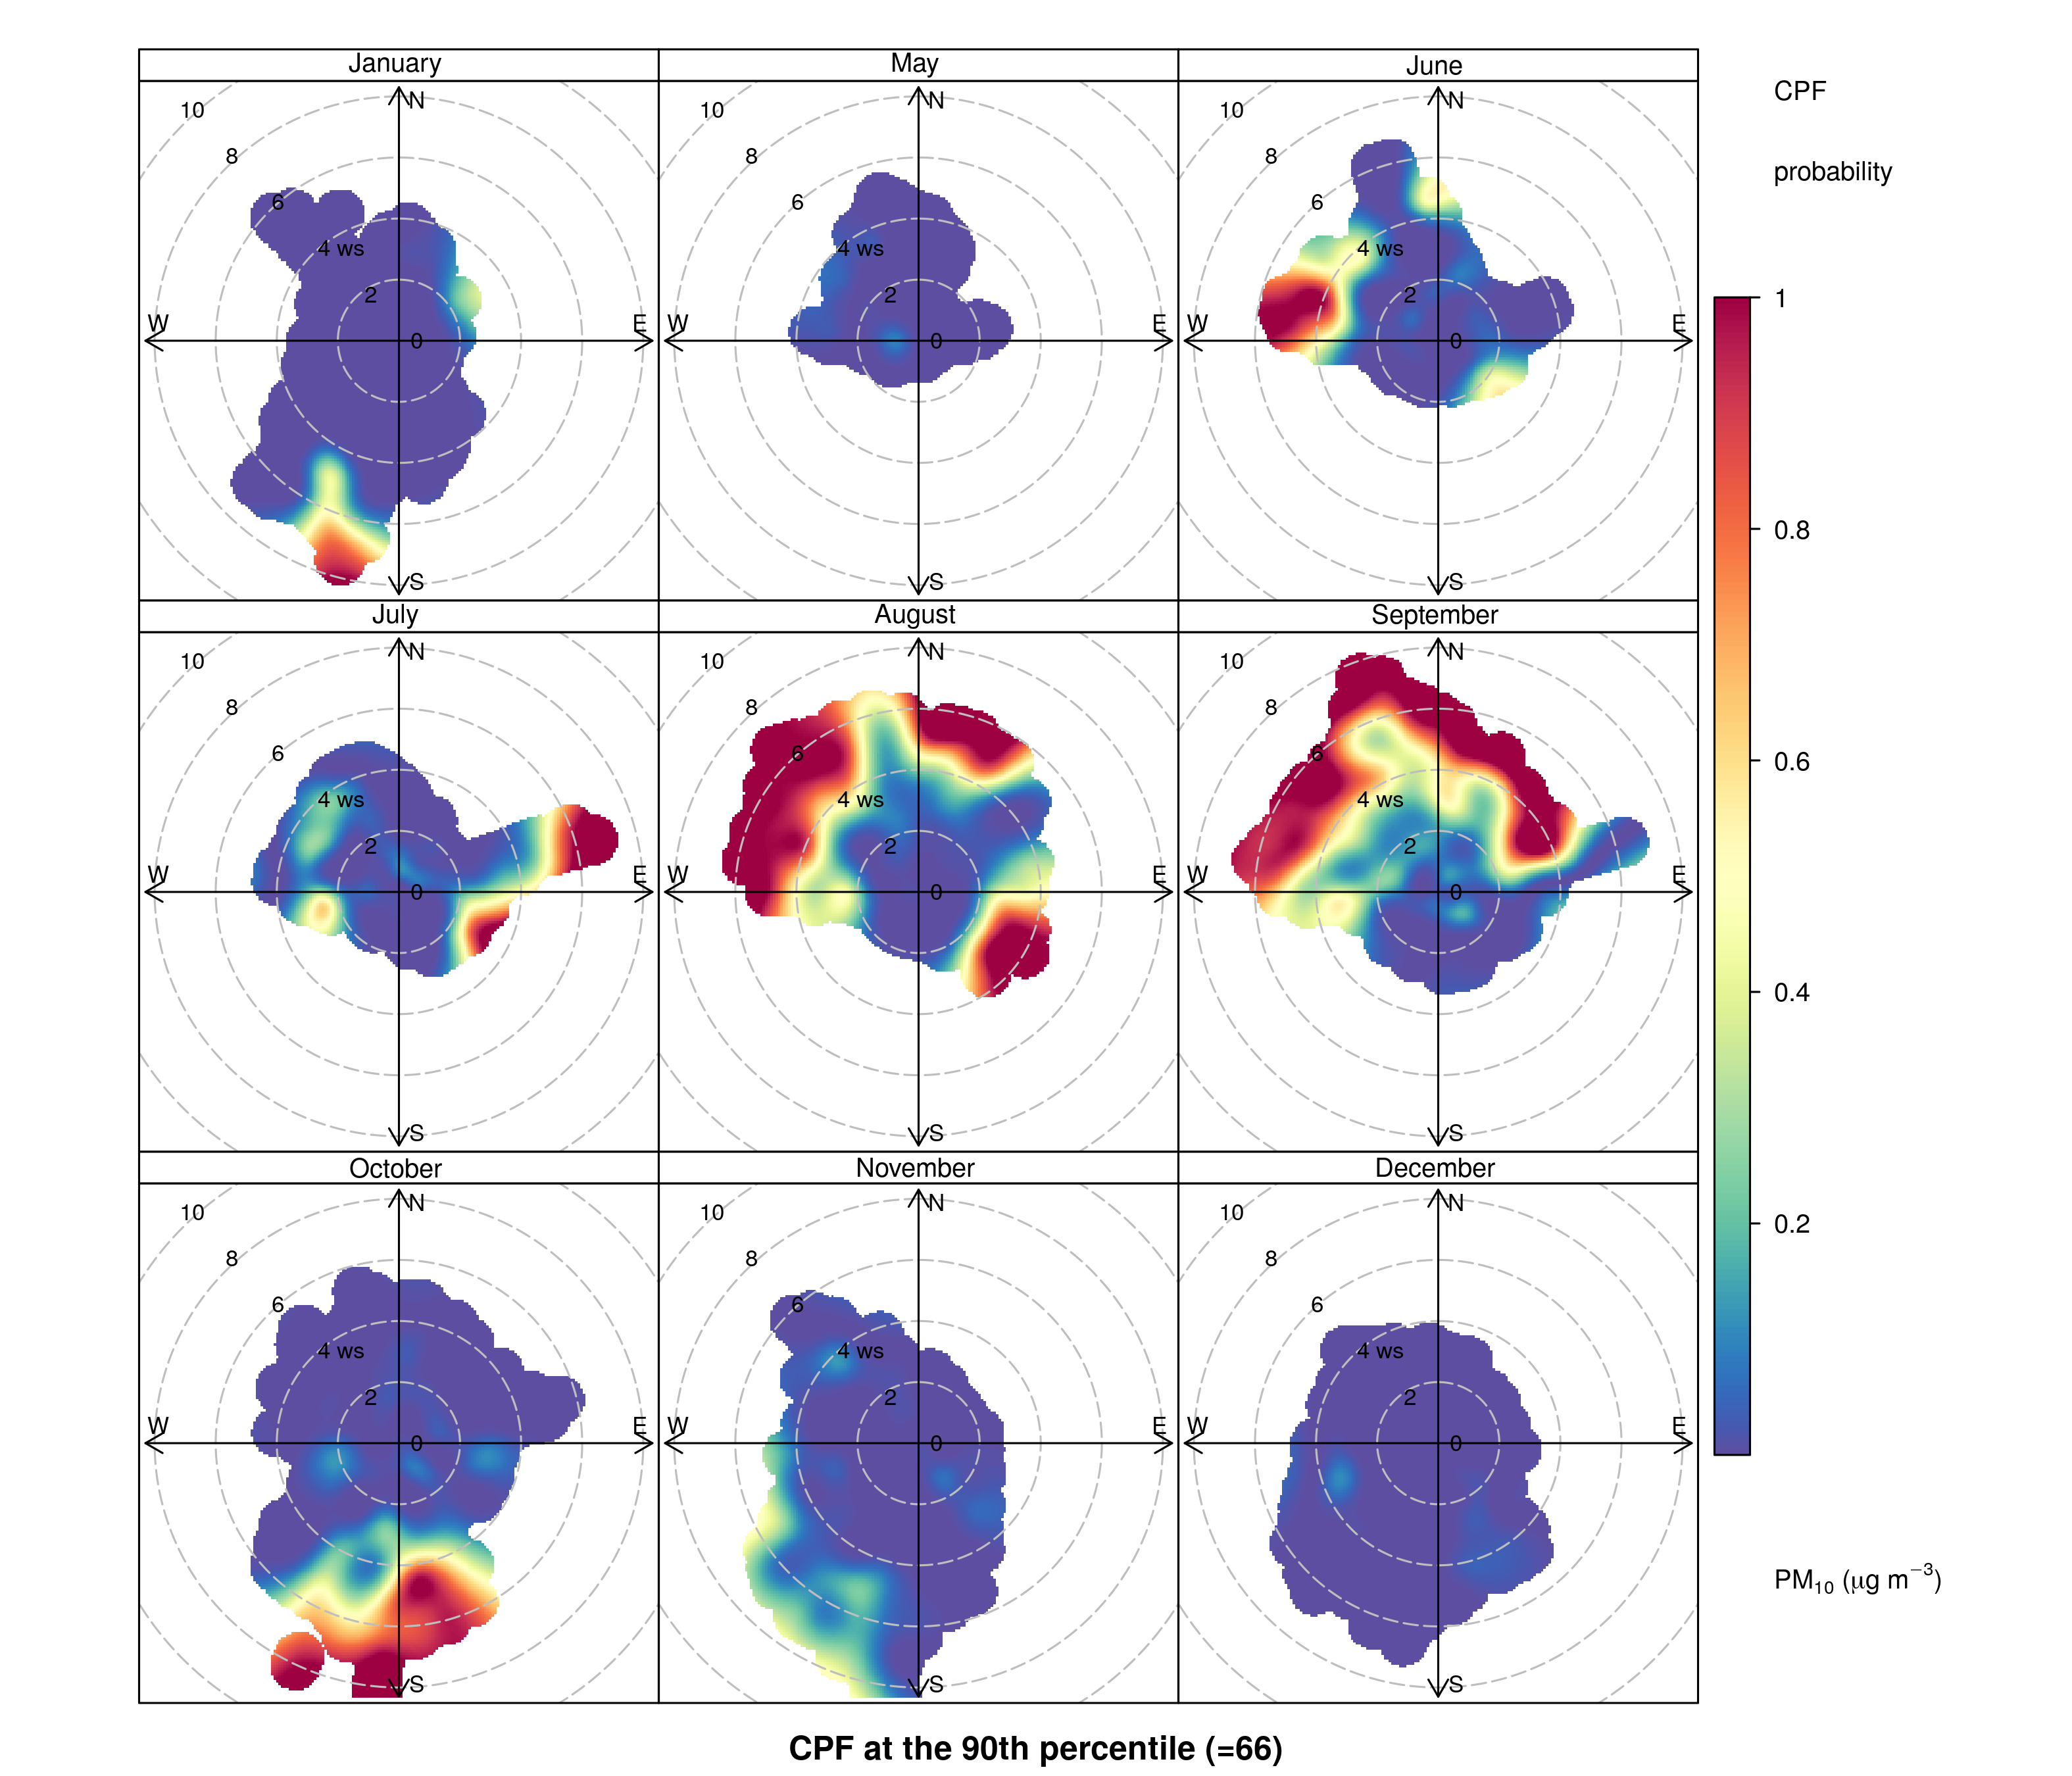
\includegraphics[width=\textwidth]{images/Wedela_PM10_polar.png}
    \caption[Polar plot for $PM_{10}$ for the sampling campaign.]{Polar plot for \gls{pm10} for the sampling campaign.}
    \label{fig:summary}
\end{figure}

\begin{figure}[!htb]
    \centering
    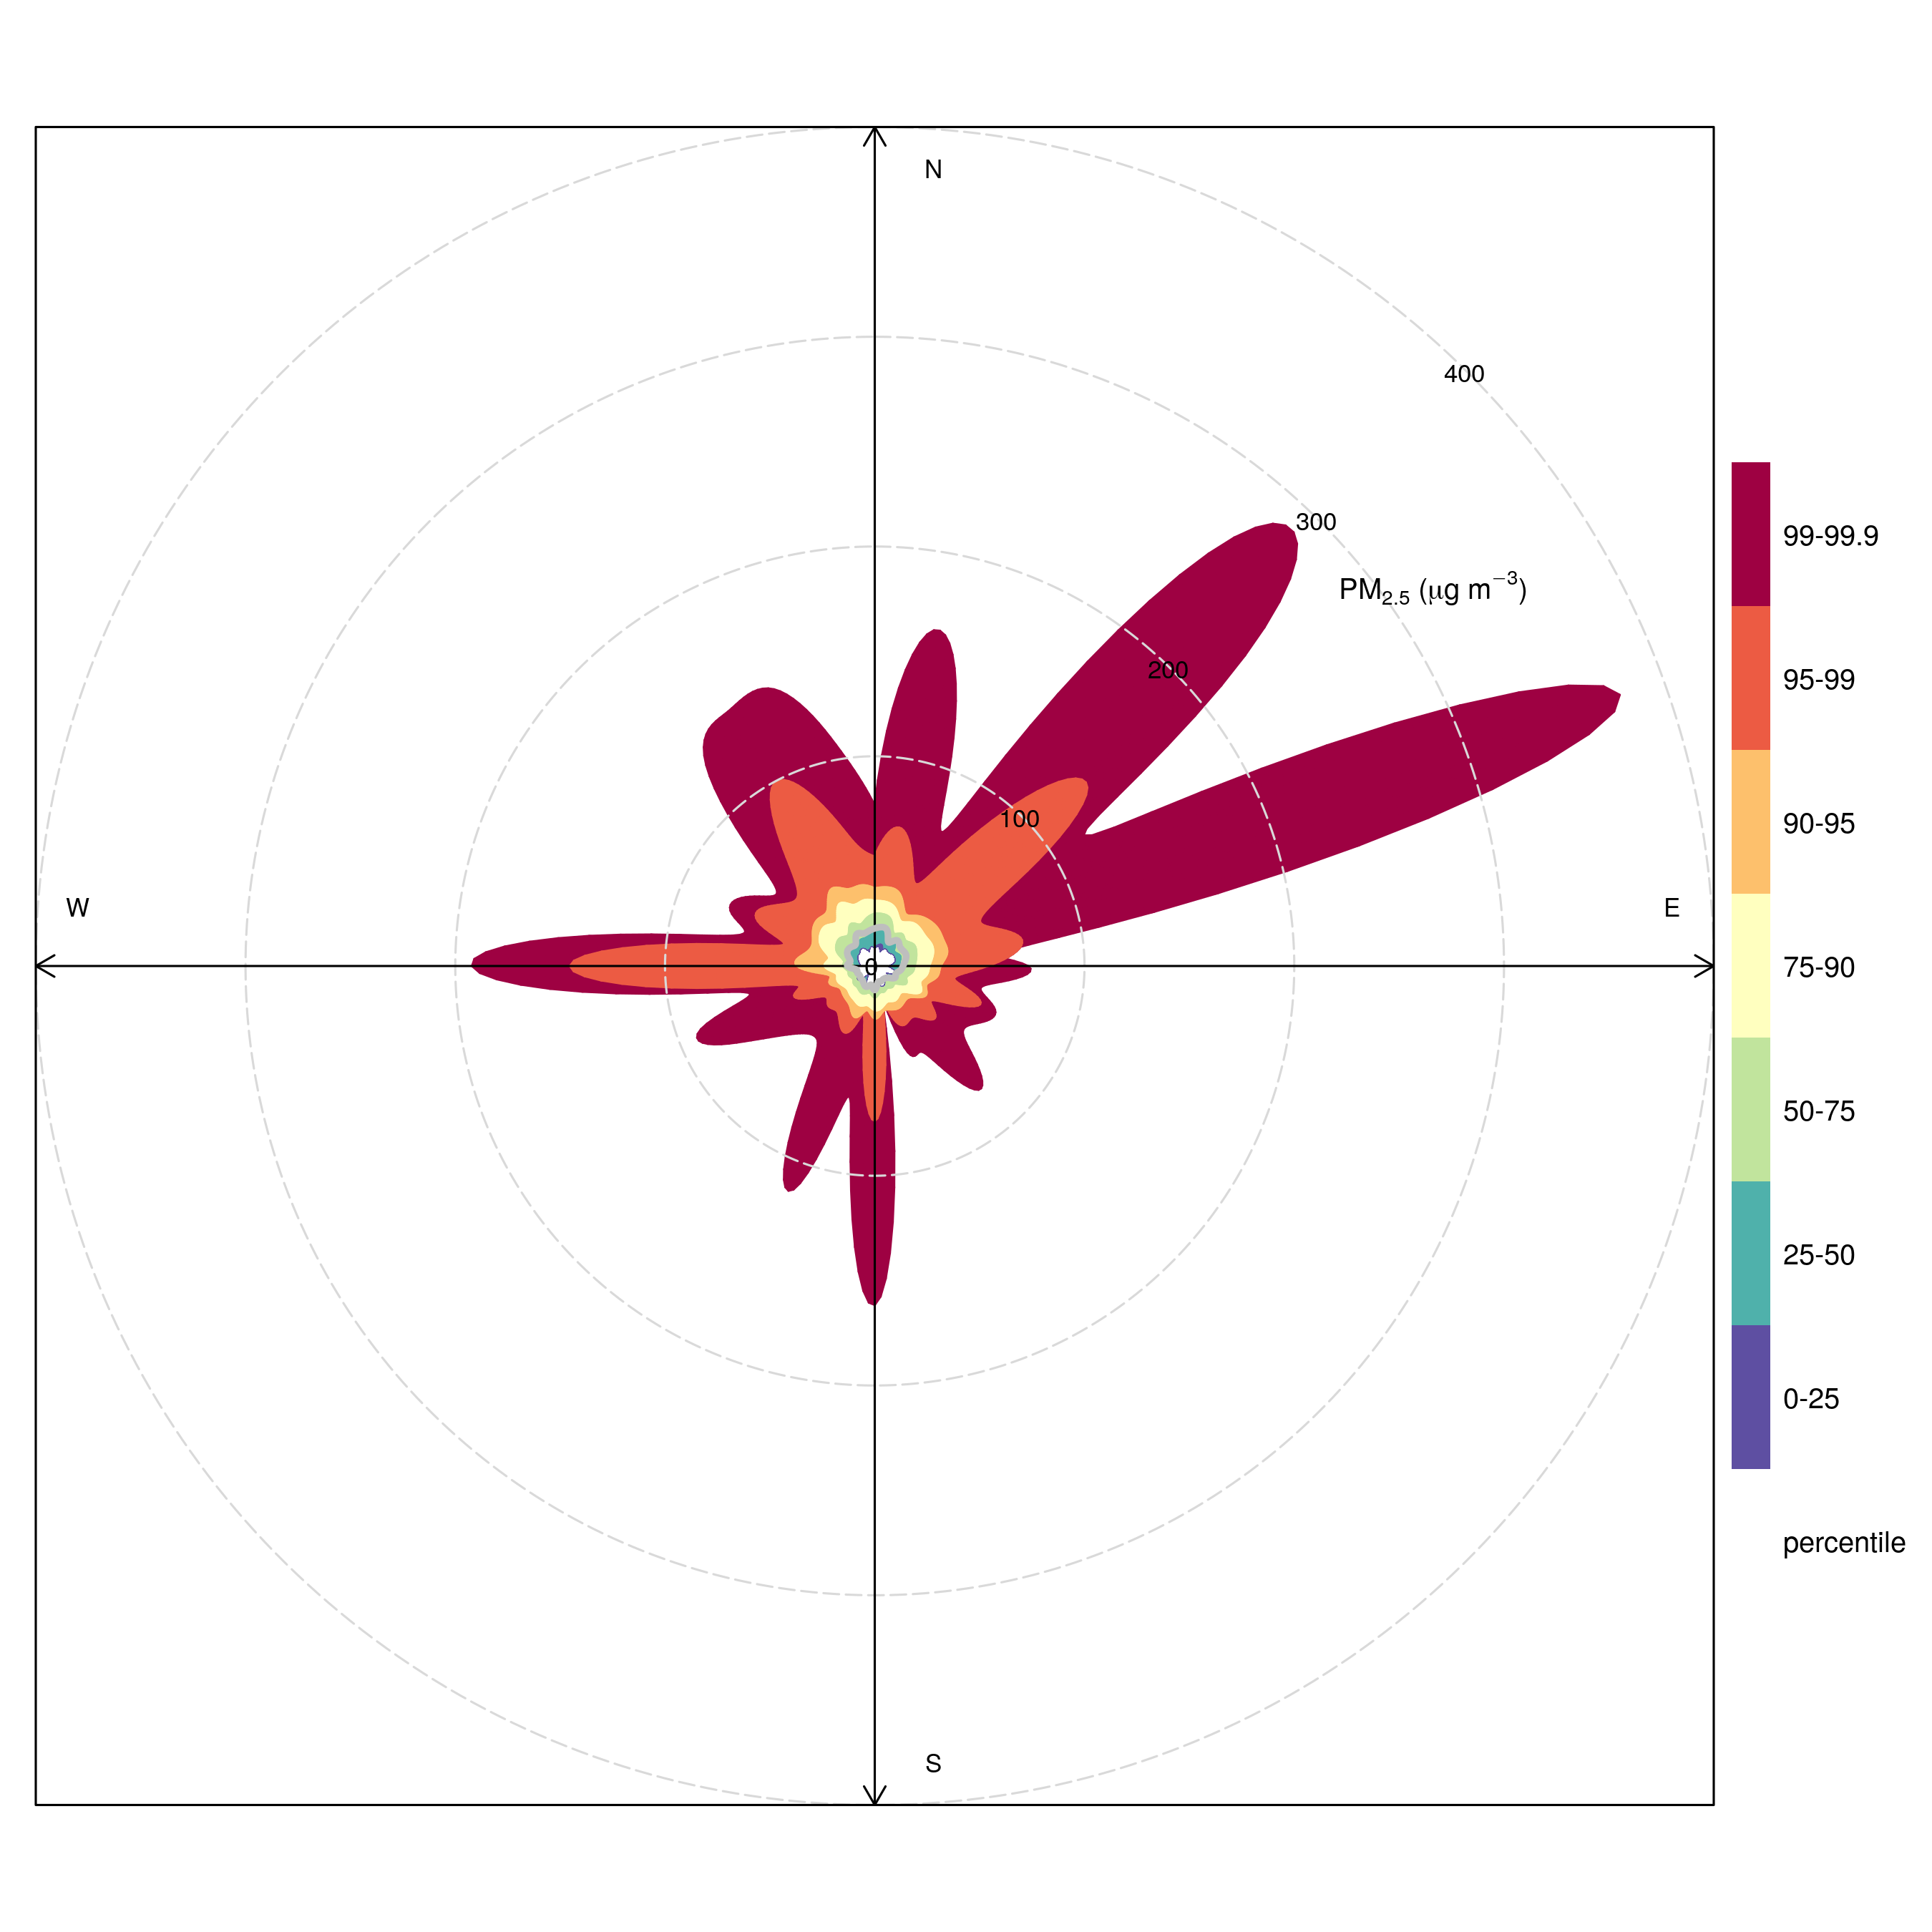
\includegraphics[width=\textwidth]{images/Wedela_PM2-5_percentileRose.png}
    \caption[Pollution rose for $PM_{2.5}$ for the sampling campaign.]{Pollution rose for \gls{pm2.5} for the sampling campaign.}
    \label{fig:summary}
\end{figure}

\begin{figure}[!htb]
    \centering
    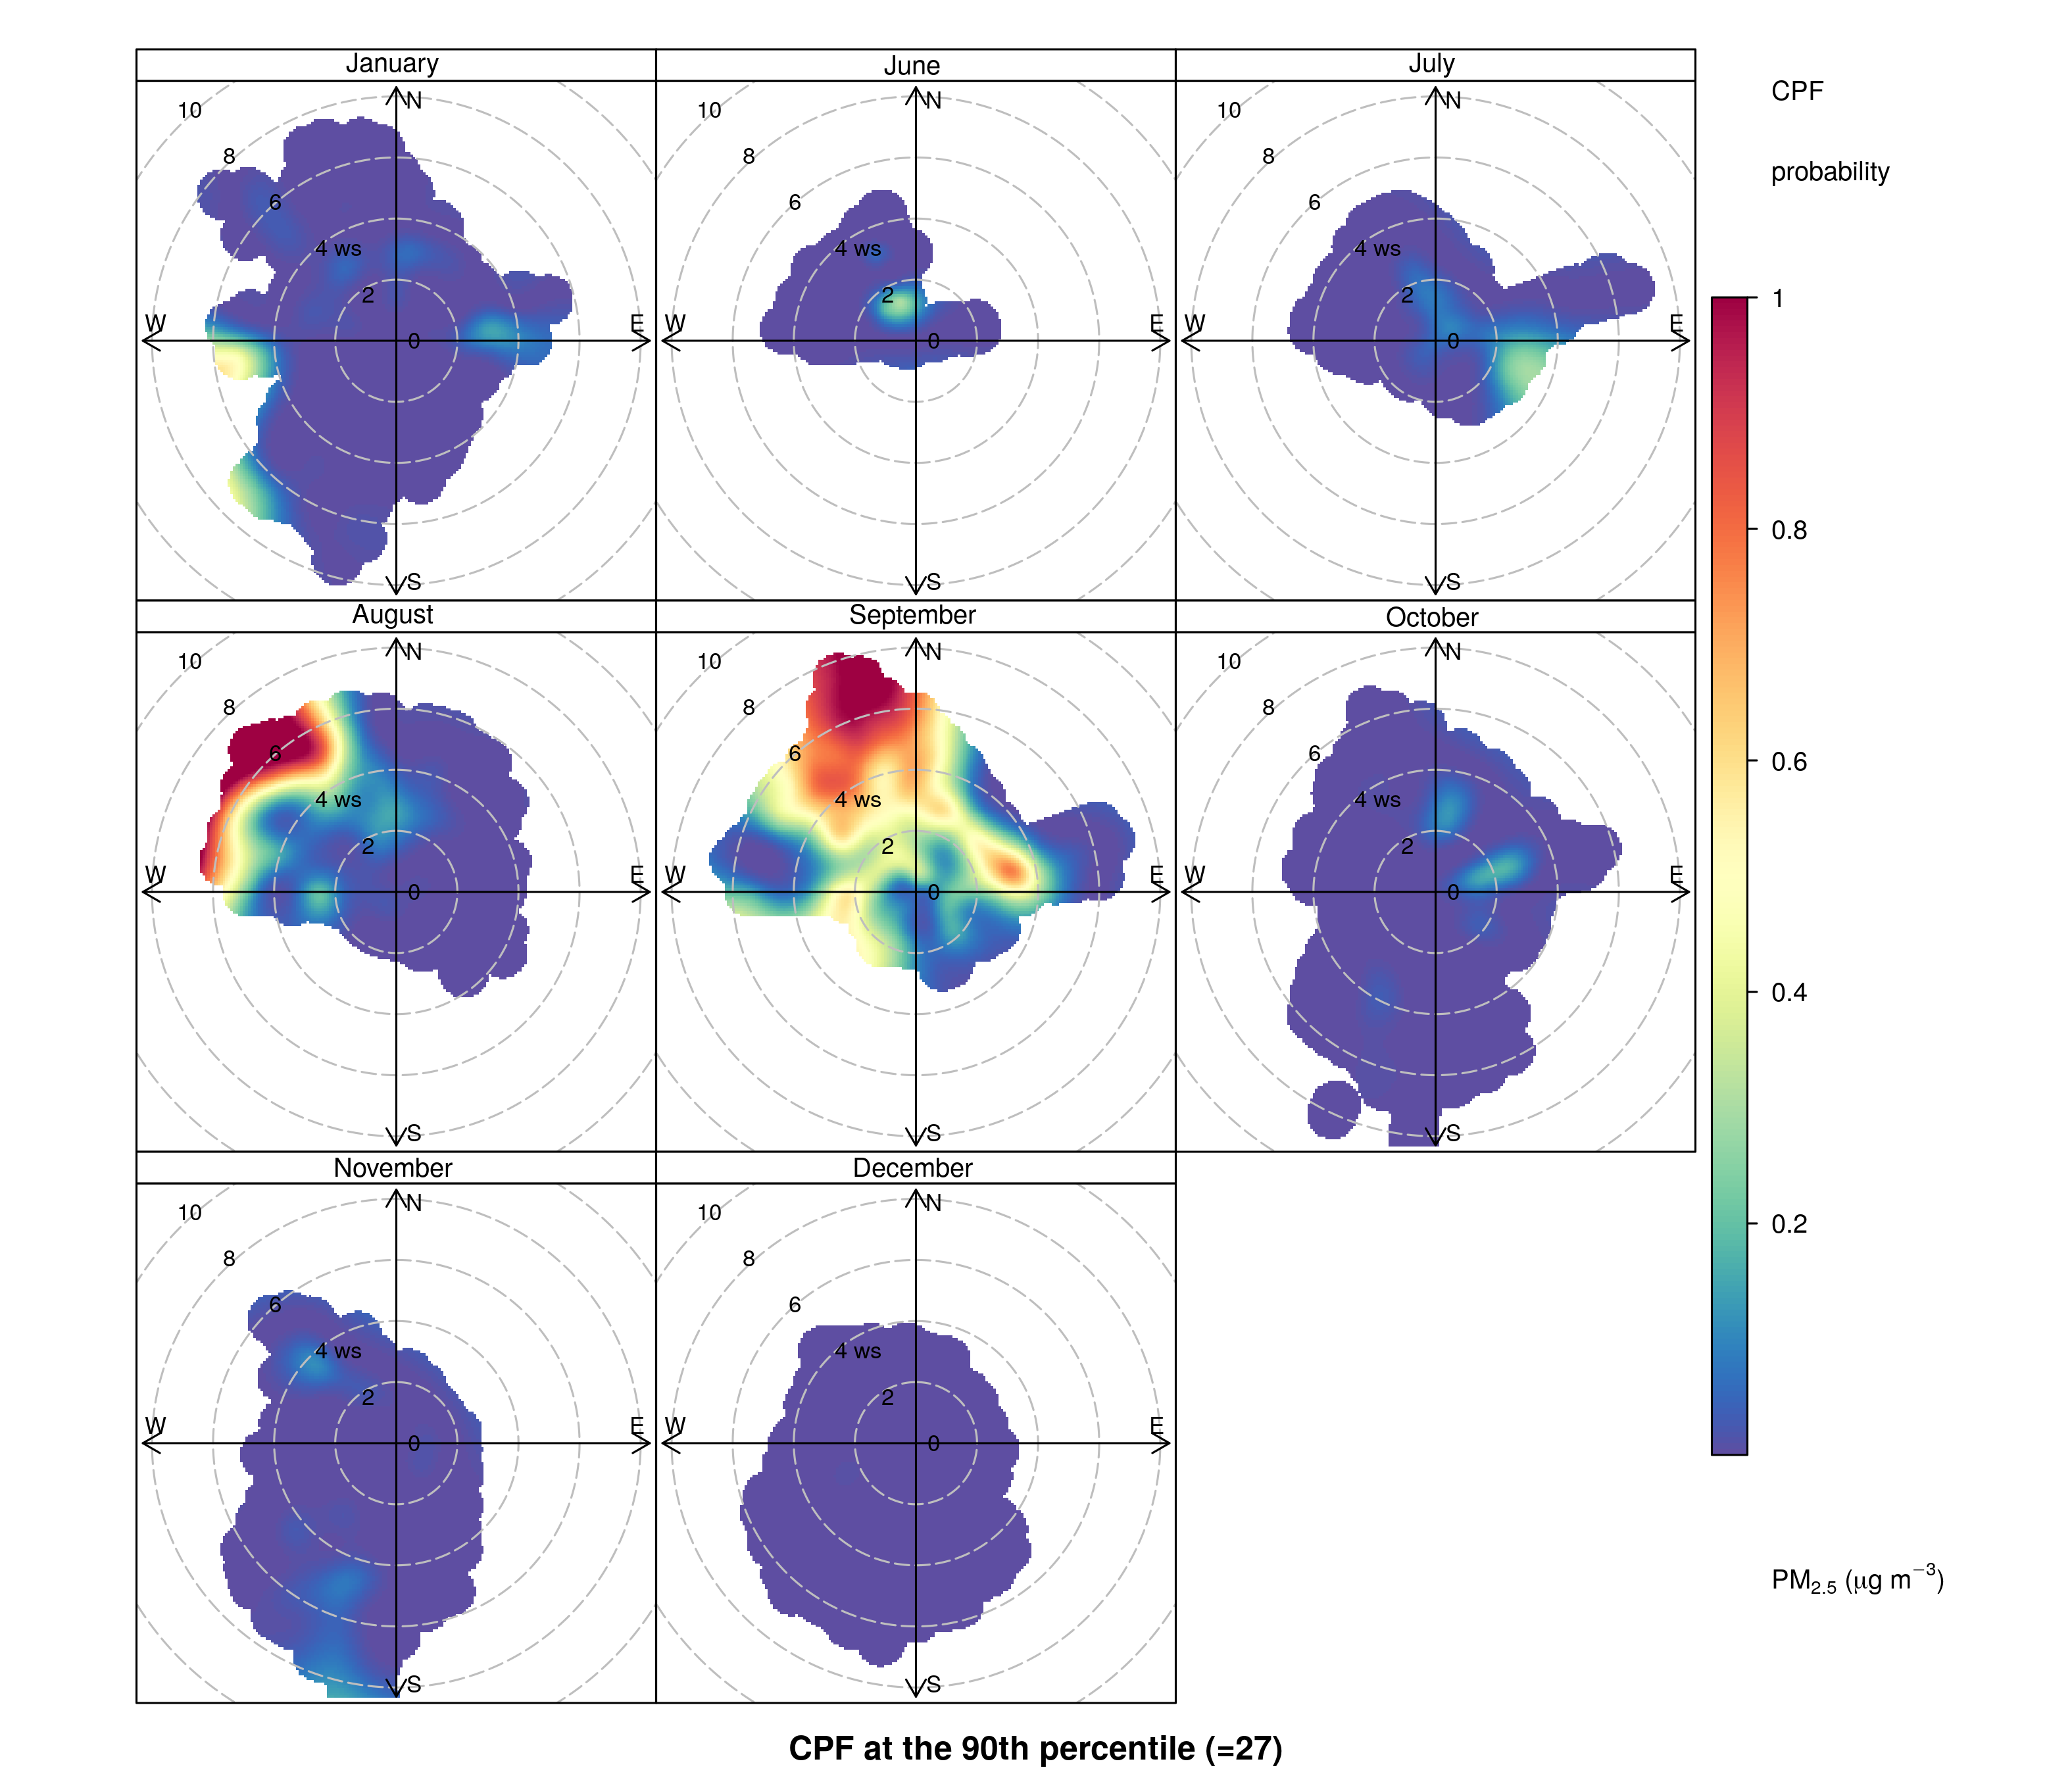
\includegraphics[width=\textwidth]{images/Wedela_PM2-5_polar.png}
    \caption[Polar plot for $PM_{2.5}$ for the sampling campaign.]{Polar plot for \gls{pm2.5} for the sampling campaign.}
    \label{fig:summary}
\end{figure}


%%%%%%%%%%%%%%%%%%%%%%%%%%%%%%%%%%%%%%%%%%%%%%%%%%%%%%%%%%%%%

\chapter{Source apportionment campaigns}
\label{sec:source}


\begin{figure}[!htb]
    \centering
    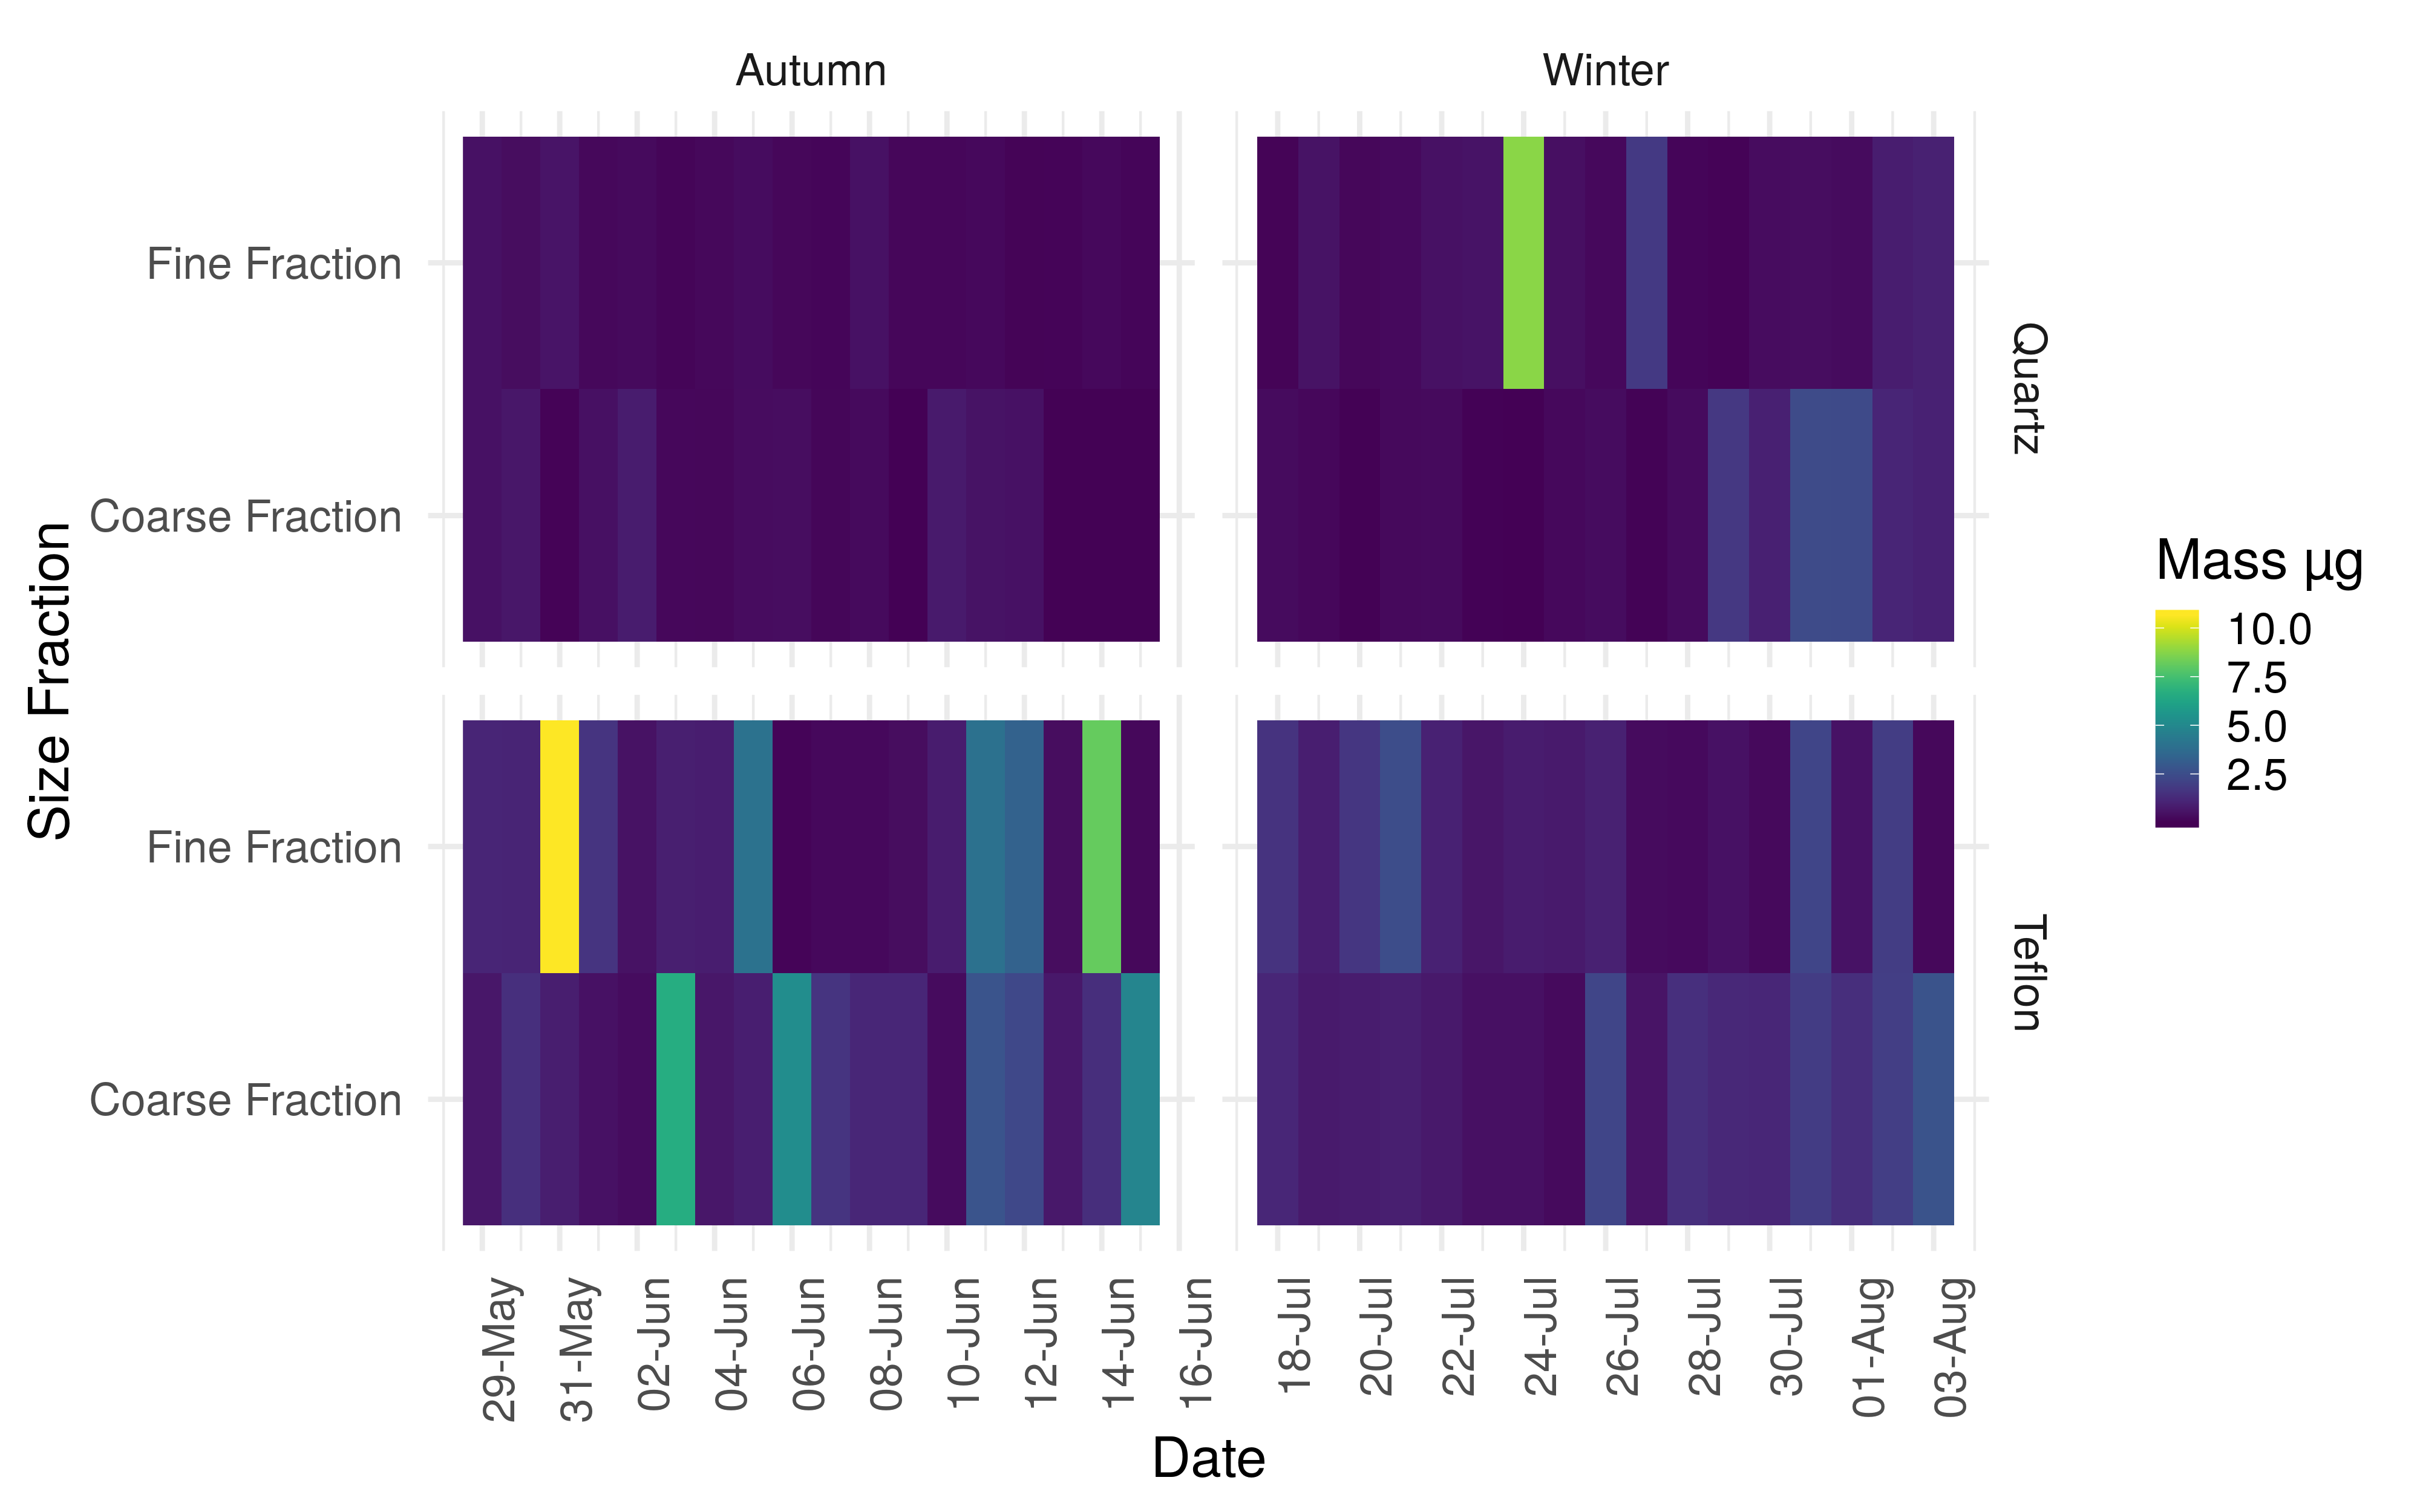
\includegraphics[width=\textwidth]{images/Density_FilterDateSizeSeason_mass.png}
    \caption{Caption}
    \label{fig:summary}
\end{figure}

\begin{figure}[!htb]
    \centering
    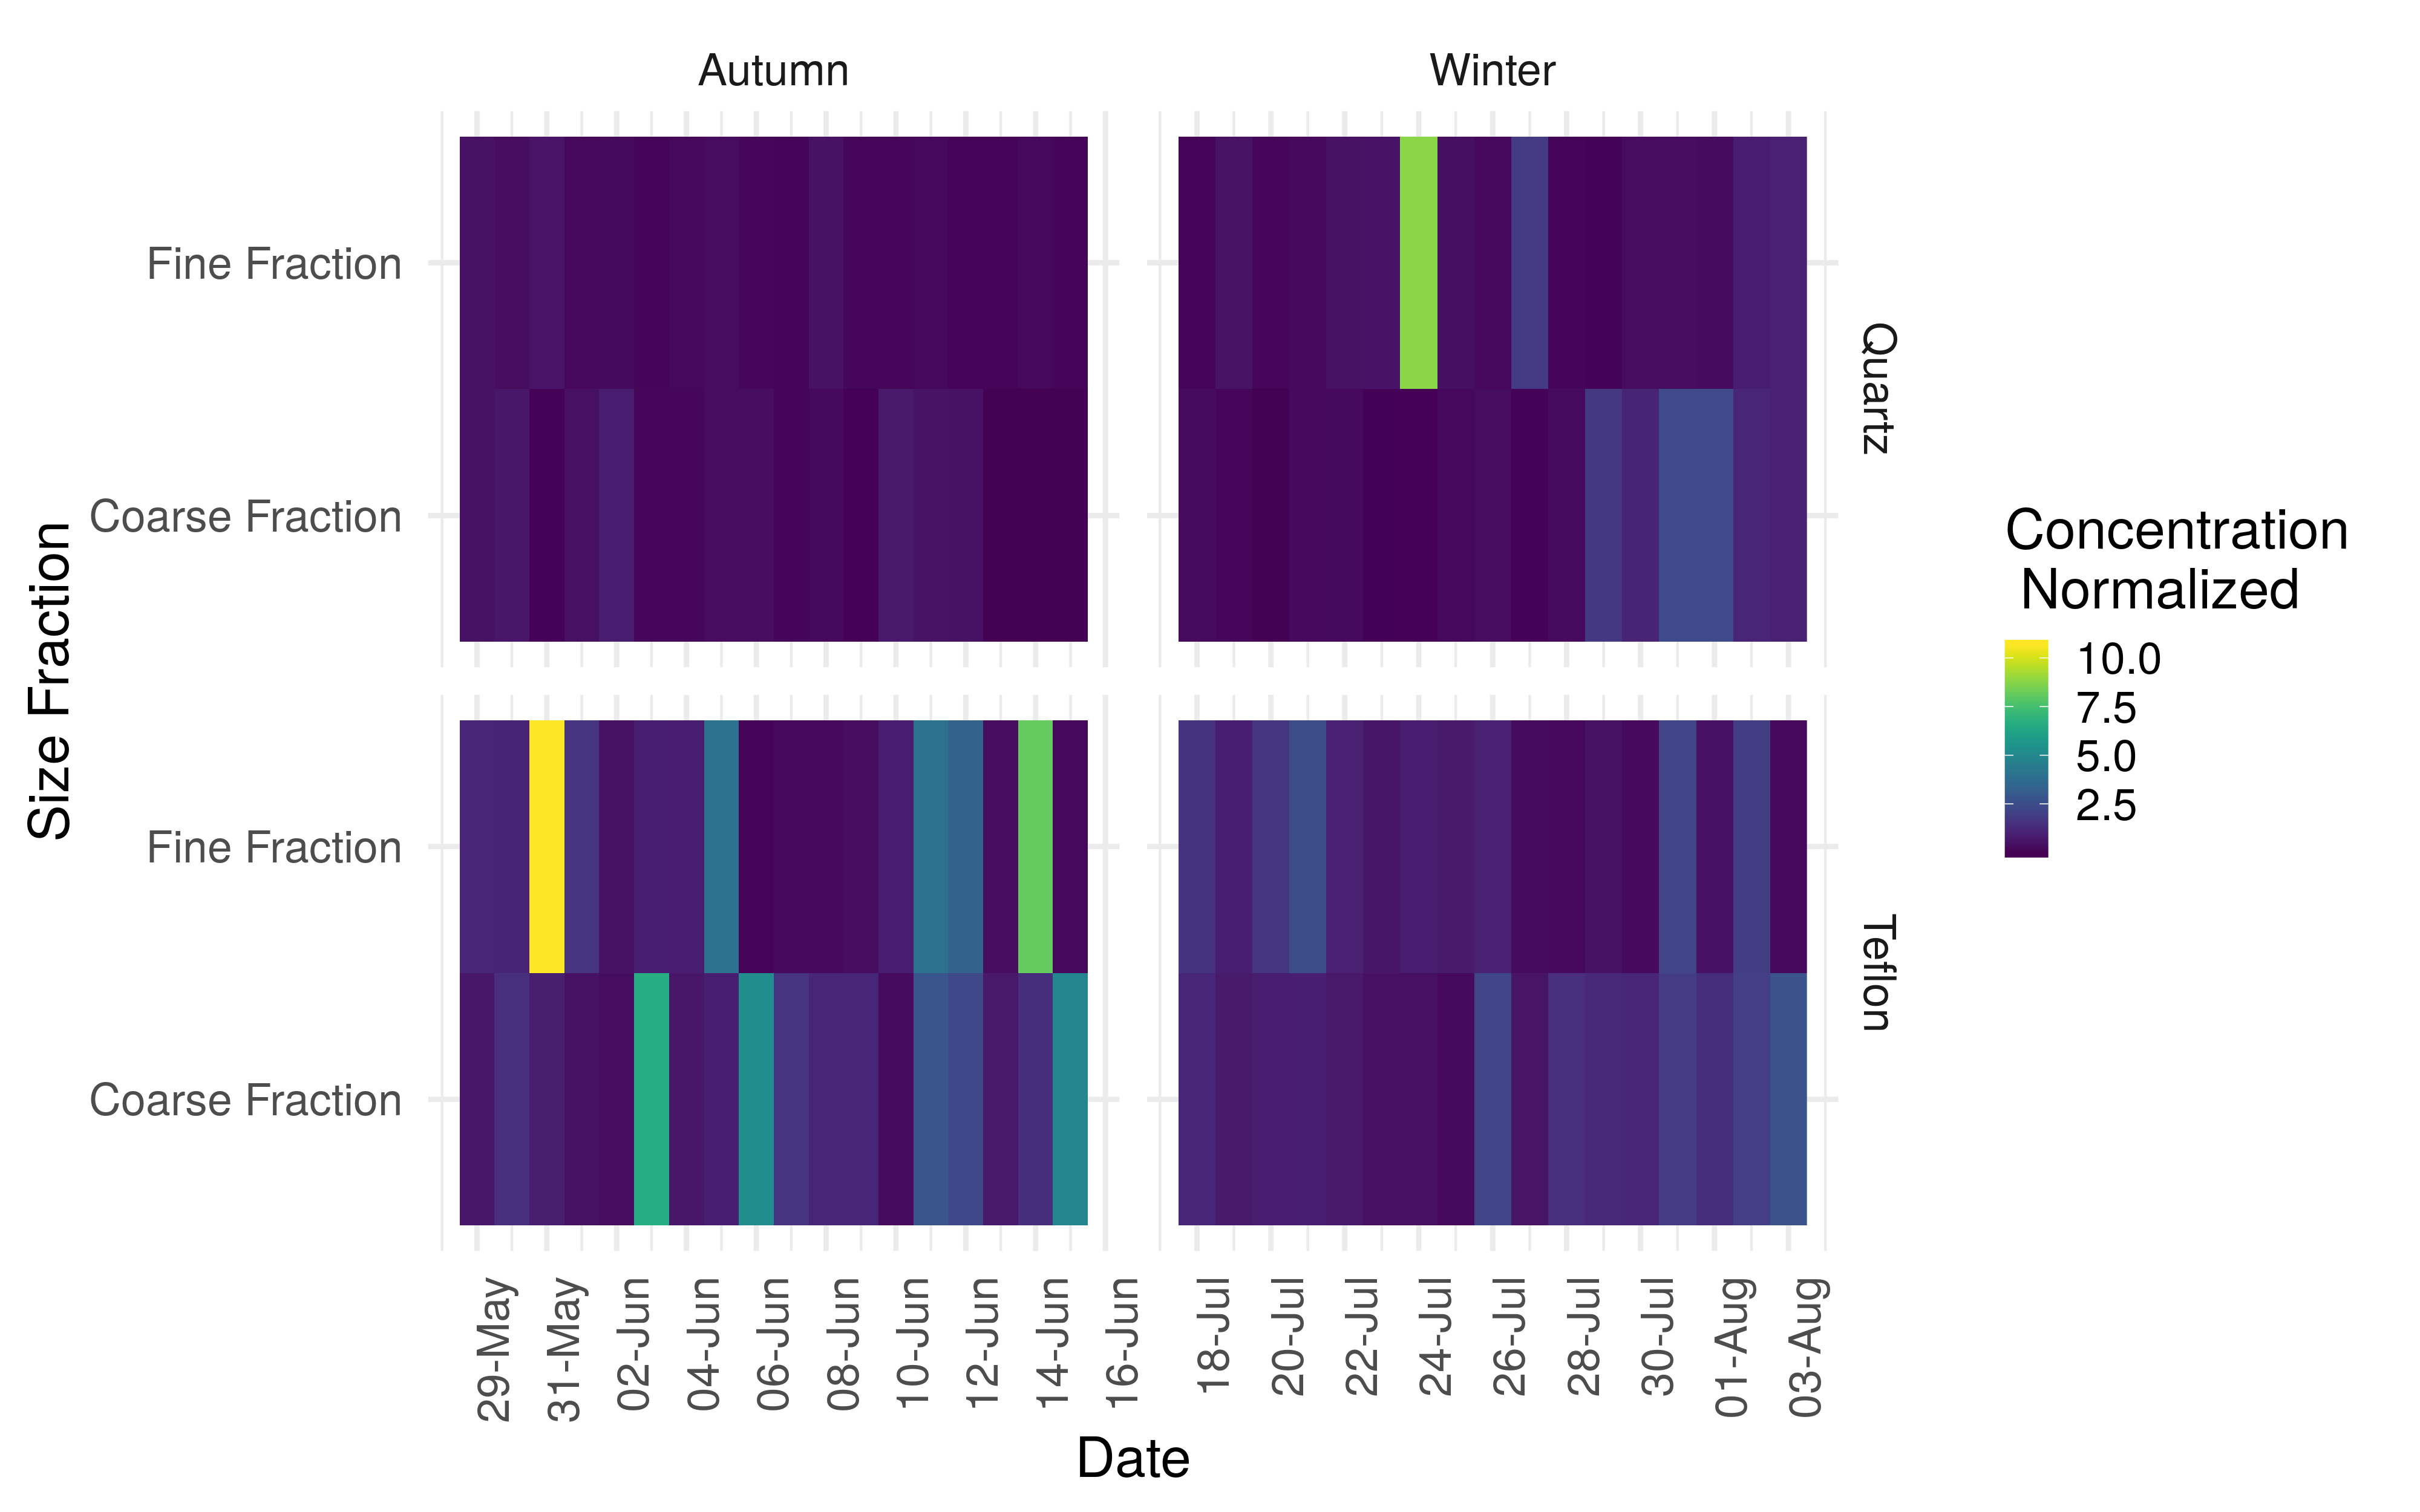
\includegraphics[width=\textwidth]{images/Density_FilterDateSizeSeason.png}
    \caption{Caption}
    \label{fig:summary}
\end{figure}

\begin{figure}[!htb]
    \centering
    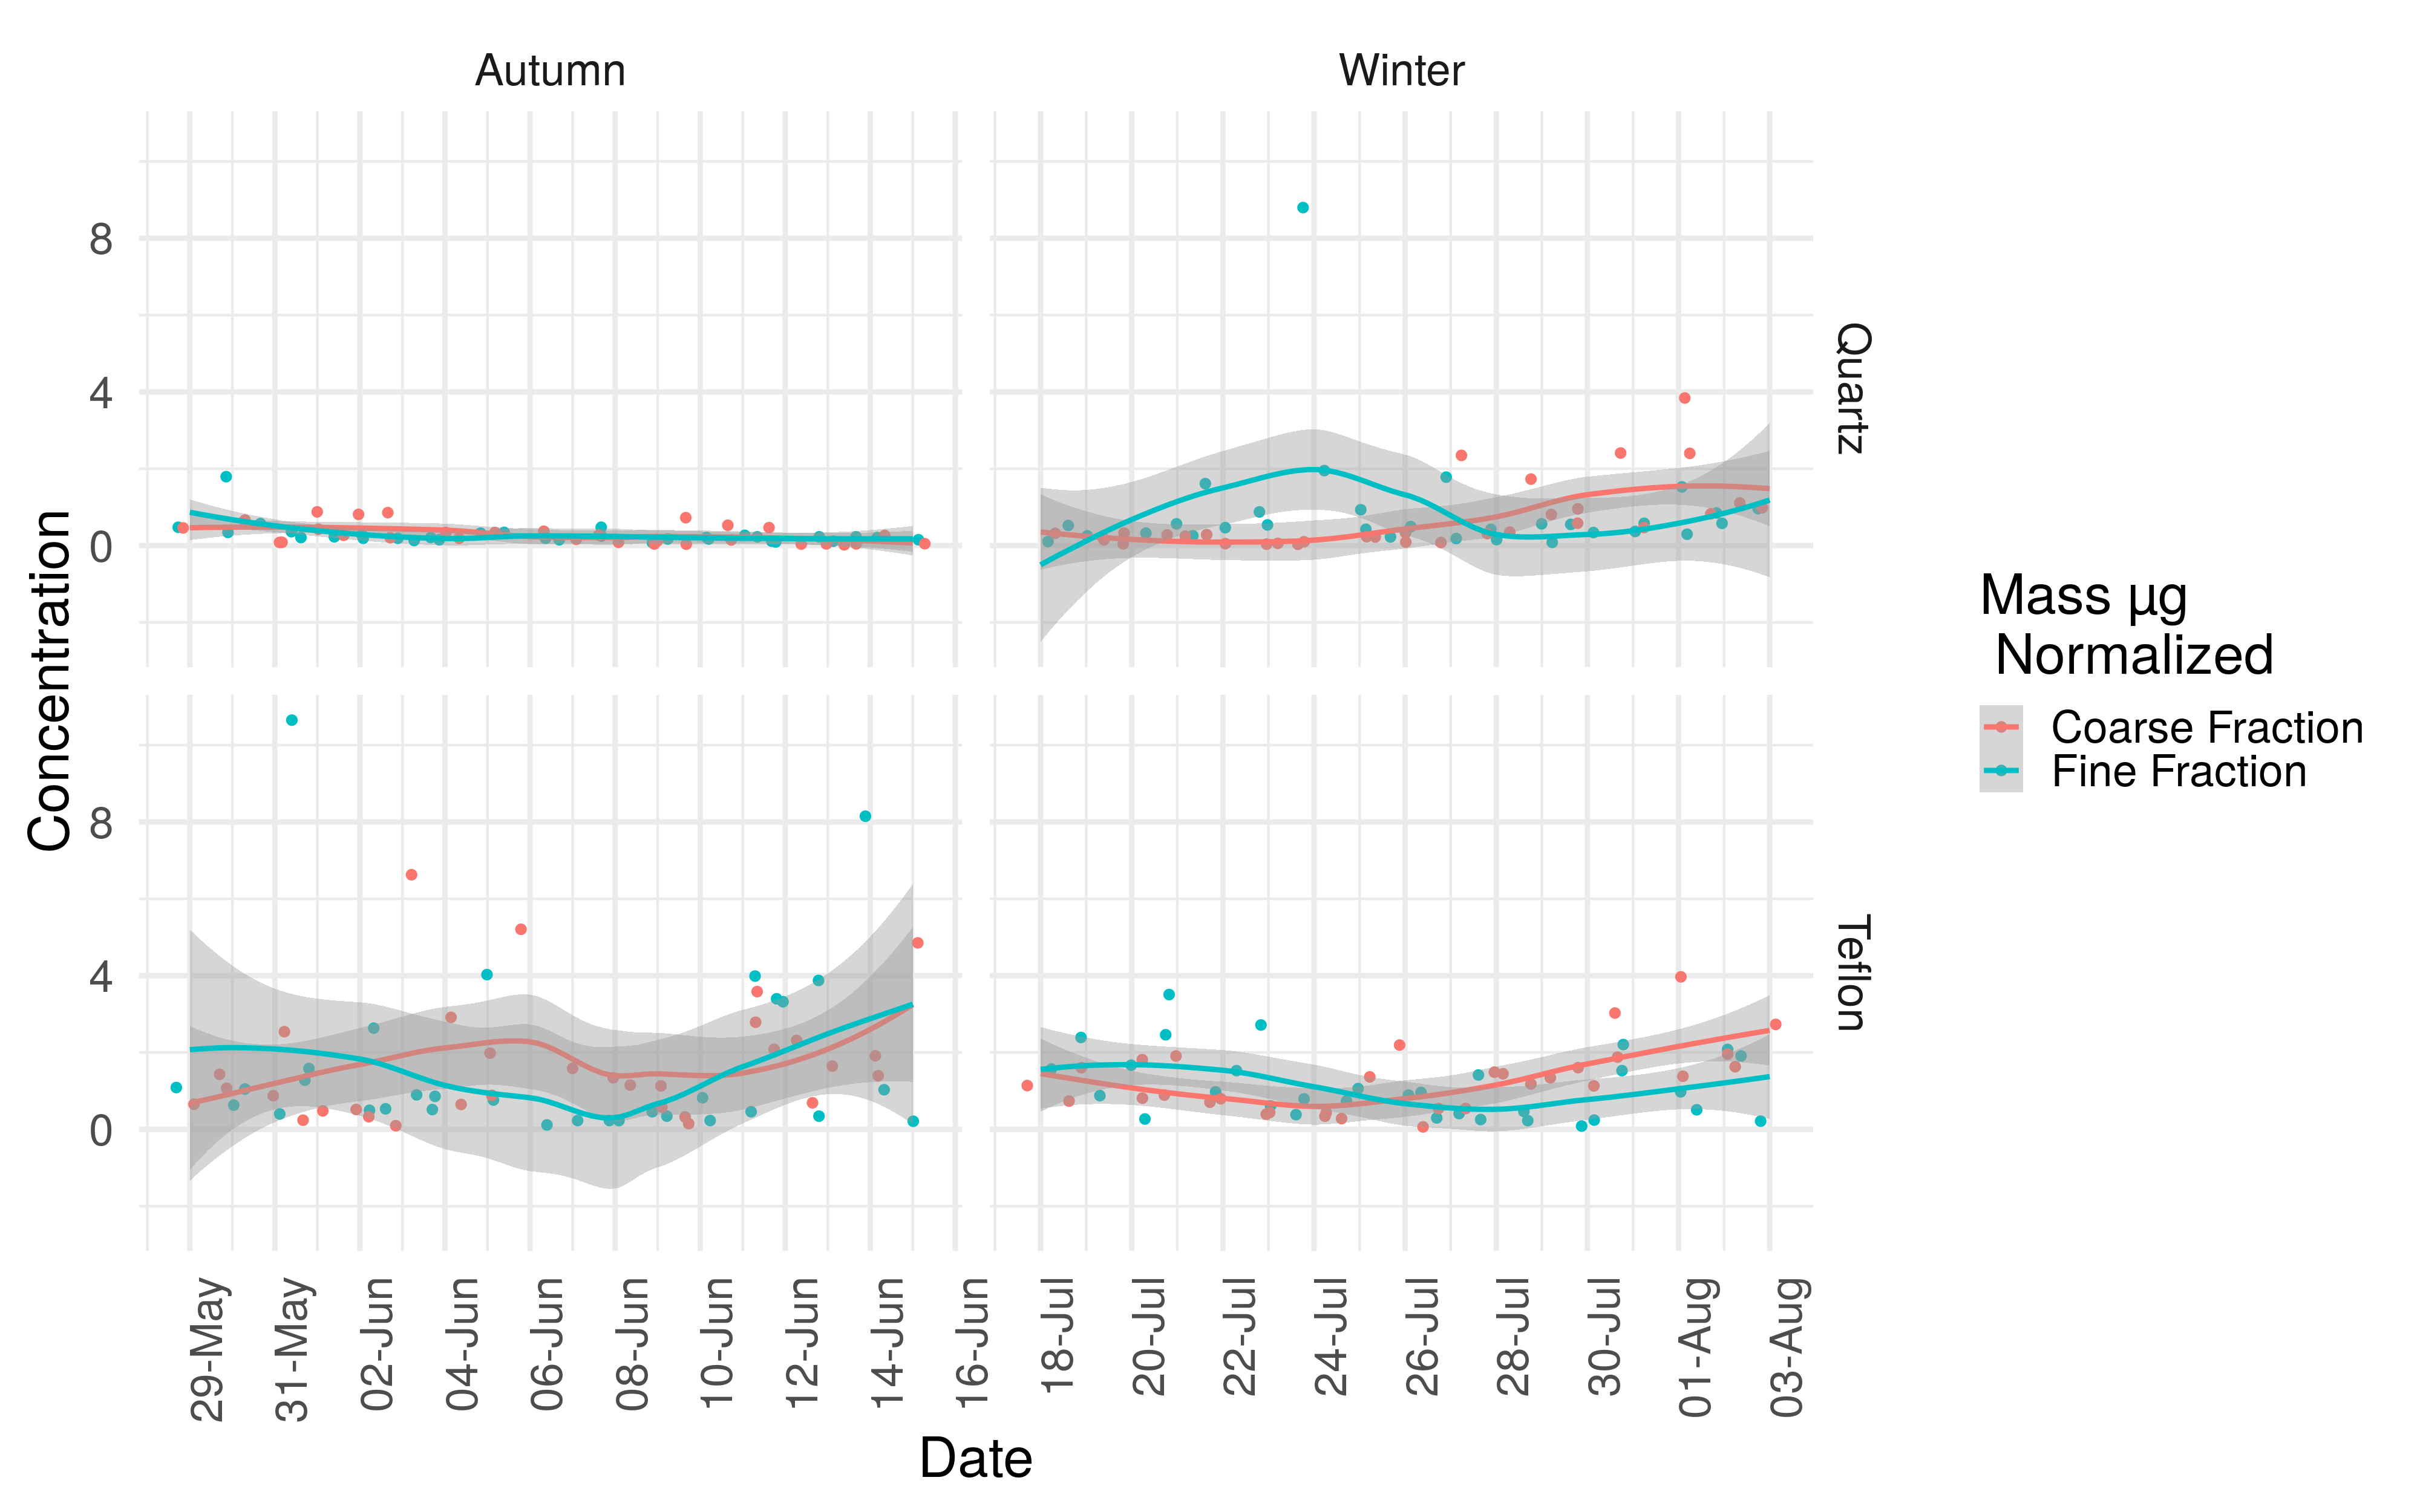
\includegraphics[width=\textwidth]{images/TS_FilterDateSizeSeason_sep_mass.png}
    \caption{Caption}
    \label{fig:summary}
\end{figure}

\begin{figure}[!htb]
    \centering
    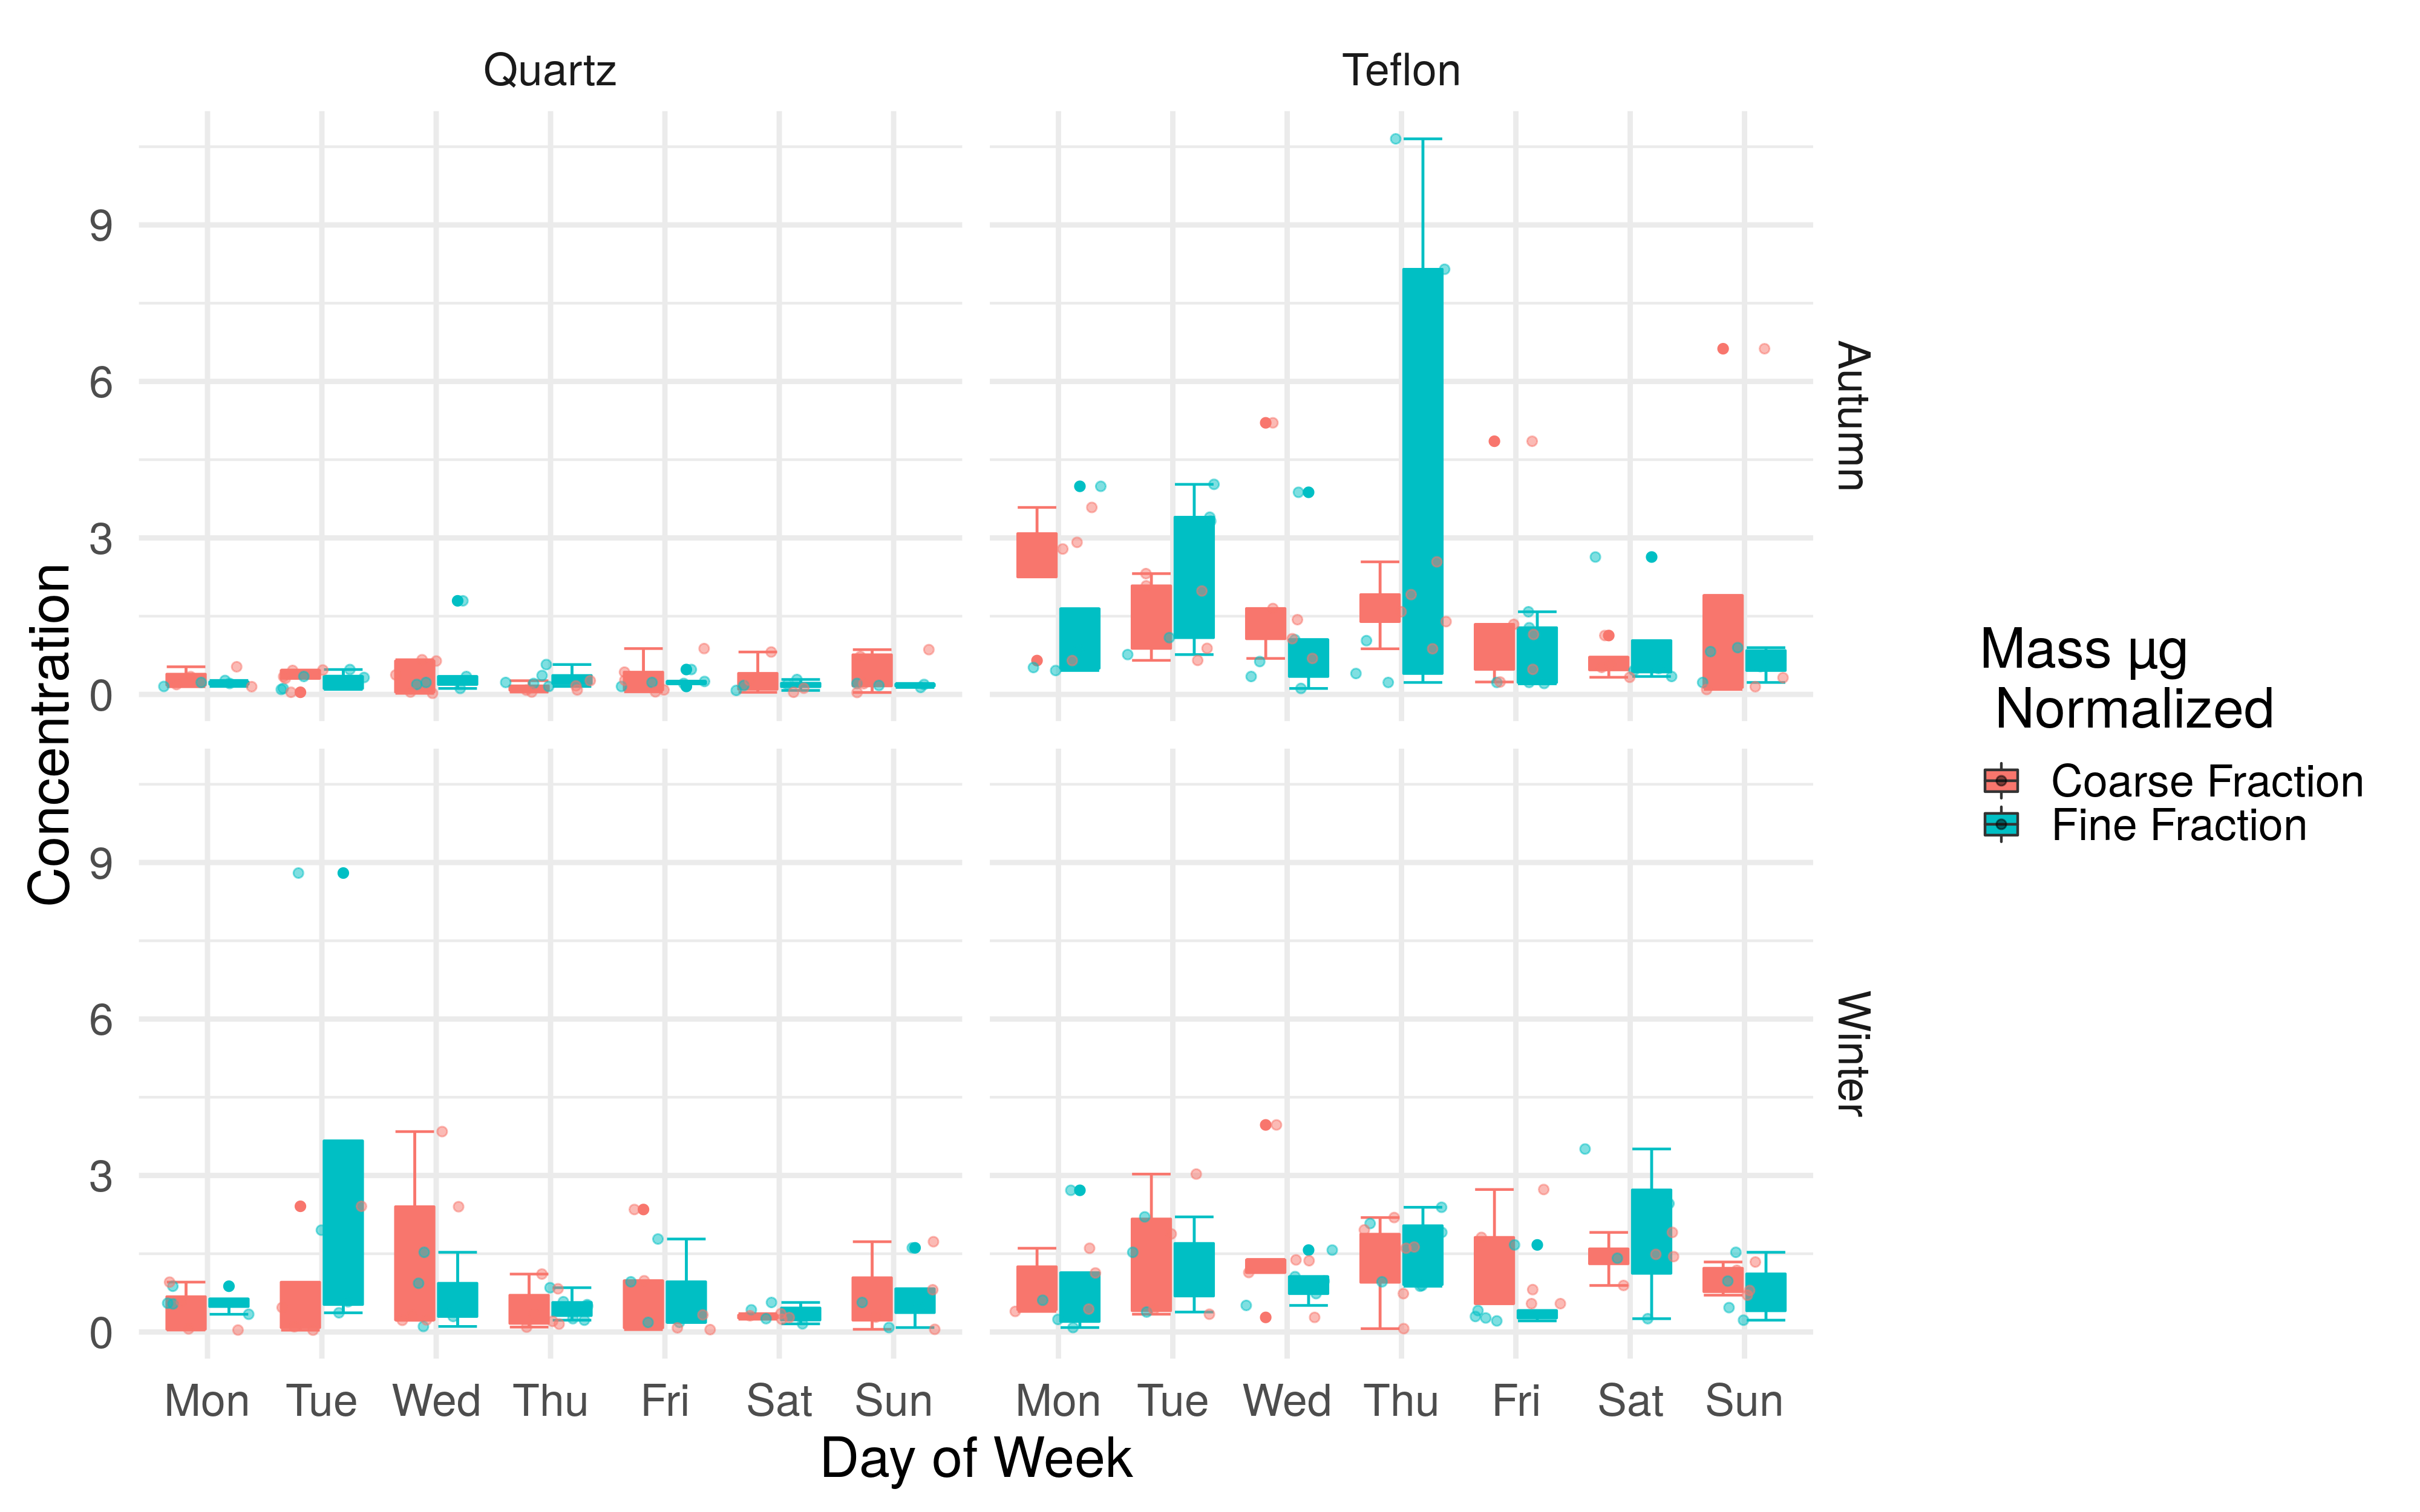
\includegraphics[width=\textwidth]{images/TS_FilterDaySizeSeason_mass.png}
    \caption{Caption}
    \label{fig:summary}
\end{figure}


\begin{figure}[!htb]
    \centering
    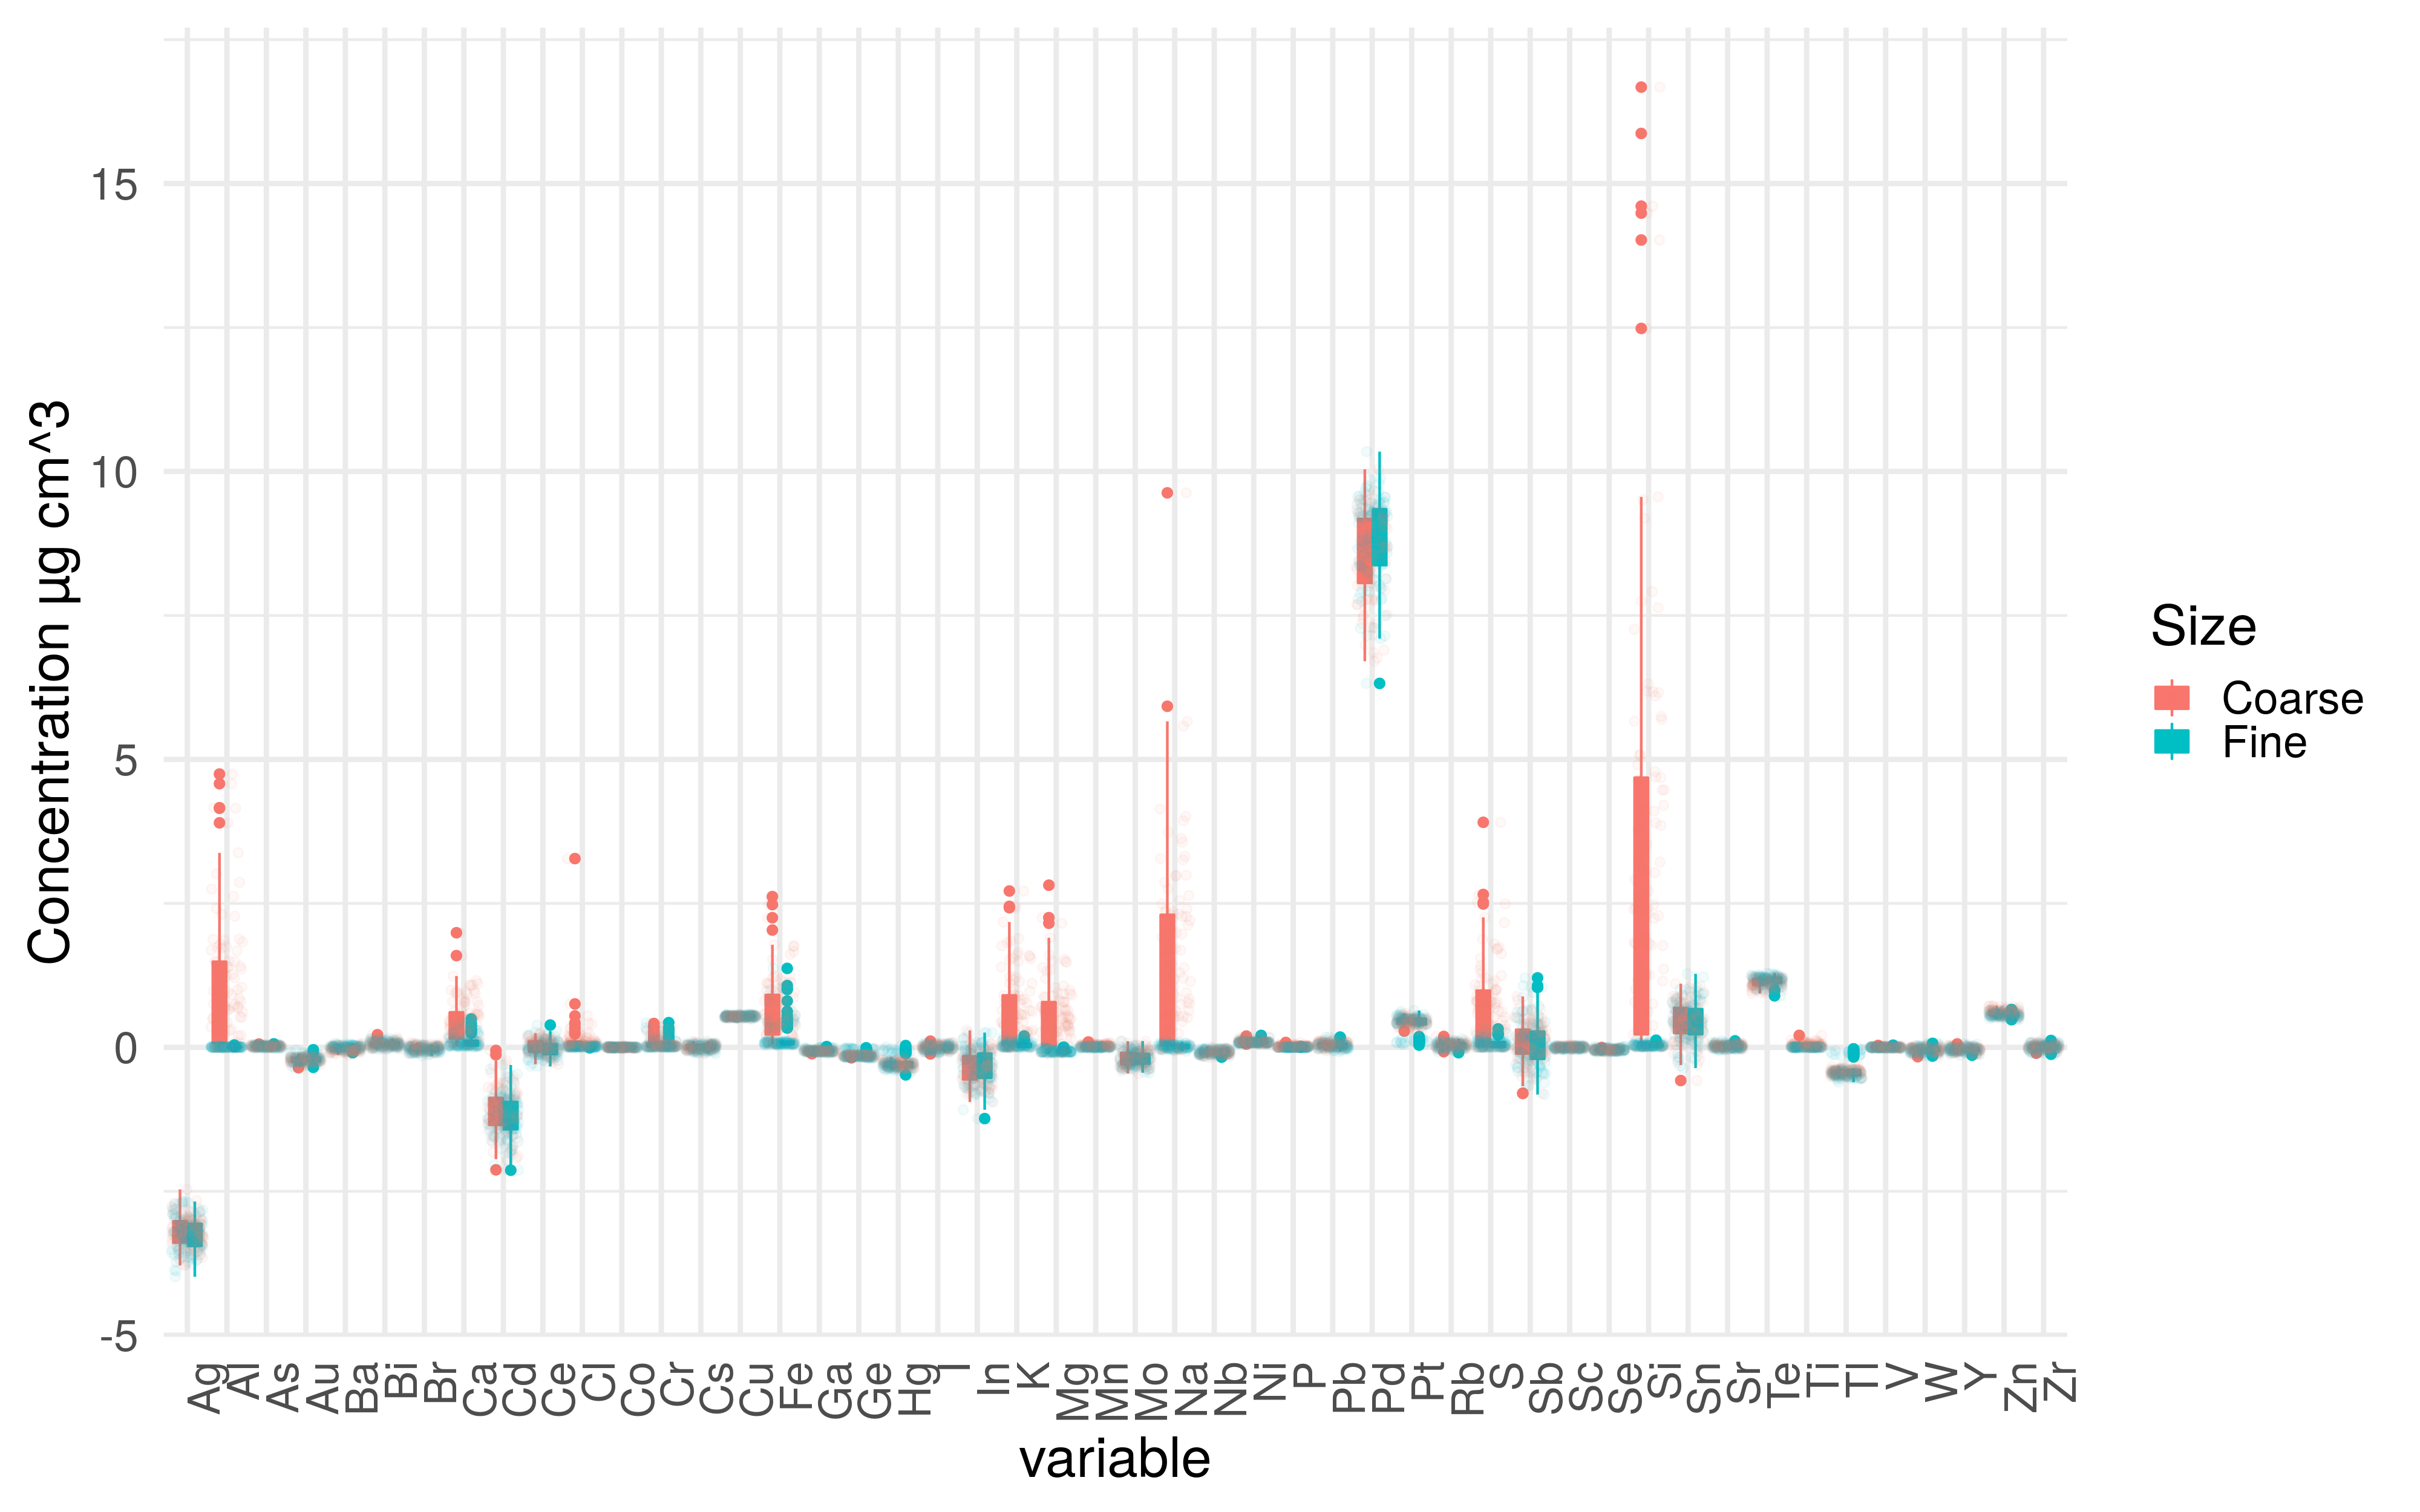
\includegraphics[width=\textwidth]{images/xrf.png}
    \caption{Caption}
    \label{fig:summary}
\end{figure}

%%%%%%%%%%%%%%%%%%%%%%%%%%%%%%%%%%%%%%%%%%%%%%%%%%%%%%%%%%%%%
\chapter{Capacity building}
\label{sec:capacity}

The project was designed to include capacity building through student participation. Four students are involved in the project. Their details are listed in Table~\ref{table:capacity}.

\begin{table}[!htbp]
\label{table:capacity}
\caption{Students participating in the study.}
\begin{center}
  \begin{tabular}{l l r l}
    \toprule
    \bfseries{Student name} & \bfseries{Degree} & \bfseries{Student nr} & \bfseries{Graduation year} \\
    \midrule
    Marvin Qhekwana & MSc & 24362042 & 2019 \\
    Thapelo Letsholo & MSc & 24308277 & 2019 \\
    Kealeboga Ntshabela & MSc & 24352829 & 2020 \\
    Prince Chidhindi & MSc & 25267108 & 2020 \\ 
    \bottomrule
  \end{tabular}
\end{center}
\end{table}
%%%%%%%%%%%%%%%%%%%%%%%%%%%%%%%%%%%%%%%%%%%%%%%%%%%%%%%%%%%%%
\chapter{Conclusions}
\label{sec:conclusions}

A project to characterize ambient \gls{pm} loading and source contribution has commenced in Wedela. The site was installed between January and April 2019. Two new MetOne E-BAM plus instruments was procured and installed in Wedela in May 2018. One is fitted with a \gls{pm2.5} sharp cut cyclone. A MetOne MSO 232 Weather station was also installed at the same site. 

Ambient \gls{pm} measurements show that the area is not currently in compliance. A total of 9 daily average exceedances were obsered for \gls{pm10} and 3 for \gls{pm2.5} during the 163 days where more than \SI{80}{\percent} data were available. The only month where daily average concentrations of \gls{pm2.5} exceeded the standards were September. \gls{pm10} daily average concentrations exceeded the standard in August and September. Another important feature of the ambient \gls{pm} concentrations is an uncharacteristic diurnal distribution. The typical bimodal distributions with peaks in the morning and afternoon that coincide with times of maximum activity in and around households. In Wedela, the \gls{pm10} has a pronounced peak during the day and \gls{pm2.5} has a small peak in the afternoon. It suggests that the sources contributing to ambient \gls{pm10} are driven by the boundary layer evolution and that different sources can be driving ambient loading of \gls{pm2.5}.

A autumn intensive source apportionment campaign was conducted between 29 May and 16 June 2018. A winter source apportionment campaign was conducted between 18 July and 3 August 2018. A third source apportionment campaign is currently underway. The fourth source apportionment campaign is being planned for September 2019, in order to coincide with the period of maximum \gls{pm2.5} and \gls{pm10} ambient concentrations.


%%%%%%%%%%%%%%%%%%%%%%%%%%%%%%%%%%%%%%%%%%%%%%%%%%%%%%%%%%%%%

\begin{spacing}{0.3}
\linespread{0.8} \normalsize
\bibliography{library}
\end{spacing}

\end{document}
